
\includegraphics[width=8.49444in,height=4.14861in]{13-MAS-MS/Cours/pandoc/media/image1.png}


\includegraphics[width=3.075in,height=3.02358in]{13-MAS-MS/Cours/pandoc/media/image3.emf}

Cycle 7 : Analyser, Modéliser, Expérimenter et Résoudre la distribution et la conversion d\textquotesingle énergie en alternatif

\textbf{Machine Asynchrone (MAS), Machine Synchrone (MS), Onduleur triphasé}

Thomas Lusseau

Lycée Robert Doisneau - ATS

\hypertarget{table-des-matiuxe8res}{%
\section*{\texorpdfstring{\textbf{Table des matières}}{Table des matières}}\label{table-des-matiuxe8res}}
\addcontentsline{toc}{section}{\textbf{Table des matières}}

\protect\hyperlink{distribution-en-triphasuxe9-utilisation-des-complexes}{1. Distribution en triphasé -- Utilisation des complexes {[}6{]}(\#distribution-en-triphasé-utilisation-des-complexes)}

\protect\hyperlink{tensions-simple-et-composuxe9e}{1.1. Tensions simple et composée {[}6{]}(\#tensions-simple-et-composée)}

\protect\hyperlink{repruxe9sentation-vectorielle-dun-signal-sinusouxefdal}{1.2. Représentation vectorielle d'un signal sinusoïdal {[}7{]}(\#représentation-vectorielle-dun-signal-sinusoïdal)}

\protect\hyperlink{puissance-ruxe9active}{1.3. Puissance réactive {[}9{]}(\#puissance-réactive)}

\protect\hyperlink{onduleur-triphasuxe9}{2. Onduleur triphasé {[}11{]}(\#onduleur-triphasé)}

\protect\hyperlink{generalites-sur-les-machines-alternatives}{3. GENERALITES SUR LES MACHINES ALTERNATIVES {[}16{]}(\#generalites-sur-les-machines-alternatives)}

\protect\hyperlink{px-stator_and_rotor_by_zureksconstitution-dune-machine-triphasuxe9e}{3.1. Constitution d'une machine triphasée {[}16{]}(\#px-stator\_and\_rotor\_by\_zureksconstitution-dune-machine-triphasée)}

\protect\hyperlink{cruxe9ation-du-champ-tournant}{3.2. Création du champ tournant {[}16{]}(\#création-du-champ-tournant)}

\protect\hyperlink{_Toc128747961}{3.3. Vitesse de synchronisme {[}18{]}(\#\_Toc128747961)}

\protect\hyperlink{_Toc128747962}{3.4. Plaque signalétique et plaque à bornes {[}20{]}(\#\_Toc128747962)}

\protect\hyperlink{couplages-uxe9toile-y-triangle-mathbfdelta}{3.5. Couplages étoile (Y) / triangle (\(\mathbf{\Delta}\)) {[}20{]}(\#couplages-étoile-y-triangle-mathbfdelta)}

\protect\hyperlink{puissances-en-triphasuxe9-uxe9quilibruxe9}{3.6. Puissances en triphasé équilibré {[}22{]}(\#puissances-en-triphasé-équilibré)}

\protect\hyperlink{couple-thermique-equivalent-cth}{3.7. Couple Thermique Equivalent (C\textsubscript{th}) {[}23{]}(\#couple-thermique-equivalent-cth)}

\protect\hyperlink{machine-asynchrone-mas}{4. Machine Asynchrone (MAS) {[}25{]}(\#machine-asynchrone-mas)}

\protect\hyperlink{glissement}{4.1. Glissement {[}25{]}(\#glissement)}

\protect\hyperlink{schuxe9ma-monophasuxe9-uxe9quivalent}{4.2. Schéma monophasé équivalent {[}25{]}(\#schéma-monophasé-équivalent)}

\protect\hyperlink{_Toc128747969}{4.3. Bilan de puissance et rendement {[}26{]}(\#\_Toc128747969)}

\protect\hyperlink{couple-uxe9lectromagnuxe9tique}{4.4. Couple électromagnétique {[}29{]}(\#couple-électromagnétique)}

\protect\hyperlink{variation-de-vitesse-dune-mas}{4.5. Variation de vitesse d'une MAS {[}31{]}(\#variation-de-vitesse-dune-mas)}

\protect\hyperlink{commande-vf-cte}{4.6. Commande V/f = cte~: {[}32{]}(\#commande-vf-cte)}

\protect\hyperlink{machine-synchrone}{5. MACHINE SYNCHRONE {[}36{]}(\#machine-synchrone)}

\protect\hyperlink{domaines-demploi}{5.1. Domaines d'emploi {[}36{]}(\#domaines-demploi)}

\protect\hyperlink{moduxe8le-simplifiuxe9-pour-un-enroulement-ou-phase}{5.2. Modèle simplifié pour un enroulement ou phase {[}37{]}(\#modèle-simplifié-pour-un-enroulement-ou-phase)}

\protect\hyperlink{diagramme-de-behn-eschenburg}{5.3. Diagramme de Behn-Eschenburg {[}37{]}(\#diagramme-de-behn-eschenburg)}

\protect\hyperlink{diagramme-de-behn-eschenburg-simplifiuxe9}{5.1. Diagramme de Behn-Eschenburg simplifié {[}38{]}(\#diagramme-de-behn-eschenburg-simplifié)}

\protect\hyperlink{relations-de-base}{5.2. Relations de base {[}38{]}(\#relations-de-base)}

\protect\hyperlink{couple-uxe9lectromagnuxe9tique-1}{5.3. Couple électromagnétique {[}38{]}(\#couple-électromagnétique-1)}

\protect\hyperlink{angle-guxe9omuxe9trique-ux3b8}{5.4. Angle géométrique θ {[}42{]}(\#angle-géométrique-θ)}

\protect\hyperlink{bilan-de-puissances}{5.5. Bilan de puissances {[}42{]}(\#bilan-de-puissances)}

\protect\hyperlink{variation-de-vitesse-de-la-ms}{5.6. Variation de vitesse de la MS {[}43{]}(\#variation-de-vitesse-de-la-ms)}

\protect\hyperlink{moteur-brushless-ou-ms-autopilotuxe9e}{5.7. Moteur Brushless ou MS autopilotée {[}43{]}(\#moteur-brushless-ou-ms-autopilotée)}

\protect\hyperlink{sources}{6. Sources {[}45{]}(\#sources)}

\protect\hyperlink{_Toc128747985}{7. Exercices du chapitre {[}46{]}(\#\_Toc128747985)}

Donner les démarches et outils nécessaires à l'étude des machines alternatives.

\textbf{Je connais~:}

\begin{longtable}[]{@{}
  >{\raggedright\arraybackslash}p{(\columnwidth - 2\tabcolsep) * \real{0.9444}}
  >{\raggedright\arraybackslash}p{(\columnwidth - 2\tabcolsep) * \real{0.0556}}@{}}
\toprule\noalign{}
\begin{minipage}[b]{\linewidth}\raggedright
\begin{itemize}
\tightlist
\item
  La relation entre tension simple et tension composée ainsi que leurs définitions
\end{itemize}
\end{minipage} & \begin{minipage}[b]{\linewidth}\raggedright
⃝
\end{minipage} \\
\midrule\noalign{}
\endhead
\bottomrule\noalign{}
\endlastfoot
\begin{minipage}[t]{\linewidth}\raggedright
\begin{itemize}
\tightlist
\item
  La définition d'un système triphasé équilibré
\end{itemize}
\end{minipage} & ⃝ \\
\begin{minipage}[t]{\linewidth}\raggedright
\begin{itemize}
\tightlist
\item
  Les représentations vectorielles et complexe d'une grandeur sinusoïdale
\end{itemize}
\end{minipage} & ⃝ \\
\begin{minipage}[t]{\linewidth}\raggedright
\begin{itemize}
\tightlist
\item
  Les impédances et admittances pour les dipôles de base (R, L,

  \begin{enumerate}
  \def\labelenumi{\Alph{enumi})}
  \setcounter{enumi}{2}
  \tightlist
  \item
  \end{enumerate}
\end{itemize}
\end{minipage} & ⃝ \\
\begin{minipage}[t]{\linewidth}\raggedright
\begin{itemize}
\tightlist
\item
  Les différents couplages pour une MAS (étoile, triangle)
\end{itemize}
\end{minipage} & ⃝ \\
\begin{minipage}[t]{\linewidth}\raggedright
\begin{itemize}
\tightlist
\item
  Les différents couplages pour une MAS (étoile, triangle)
\end{itemize}
\end{minipage} & ⃝ \\
\begin{minipage}[t]{\linewidth}\raggedright
\begin{itemize}
\tightlist
\item
  Les définitions des puissances active, réactive et apparente en triphasé et le théorème de Boucherot
\end{itemize}
\end{minipage} & ⃝ \\
\begin{minipage}[t]{\linewidth}\raggedright
\begin{itemize}
\tightlist
\item
  Les relations fondamentales de la MAS (vitesse de synchronisme, glissement,\ldots)
\end{itemize}
\end{minipage} & ⃝ \\
\begin{minipage}[t]{\linewidth}\raggedright
\begin{itemize}
\tightlist
\item
  Le bilan de puissance de la MAS et les relations des différentes puissances
\end{itemize}
\end{minipage} & ⃝ \\
\begin{minipage}[t]{\linewidth}\raggedright
\begin{itemize}
\tightlist
\item
  La méthode pour déterminer l'expression du couple électromagnétique à partir du schéma équivalent
\end{itemize}
\end{minipage} & ⃝ \\
\begin{minipage}[t]{\linewidth}\raggedright
\begin{itemize}
\tightlist
\item
  Les différents moyens permettant de faire varier la vitesse d'une MAS
\end{itemize}
\end{minipage} & ⃝ \\
\begin{minipage}[t]{\linewidth}\raggedright
\begin{itemize}
\tightlist
\item
  Le schéma équivalent monophasé de Behn-Eschenburg pour la MS
\end{itemize}
\end{minipage} & ⃝ \\
\begin{minipage}[t]{\linewidth}\raggedright
\begin{itemize}
\tightlist
\item
  La méthode pour tracer les diagrammes vectoriels et déterminer les différentes grandeurs du schéma de Behn-Eschenburg
\end{itemize}
\end{minipage} & ⃝ \\
\begin{minipage}[t]{\linewidth}\raggedright
\begin{itemize}
\tightlist
\item
  Les relations fondamentales de la MS
\end{itemize}
\end{minipage} & ⃝ \\
\begin{minipage}[t]{\linewidth}\raggedright
\begin{itemize}
\tightlist
\item
  La méthode pour déterminer l'expression du couple électromagnétique de la MS
\end{itemize}
\end{minipage} & ⃝ \\
\begin{minipage}[t]{\linewidth}\raggedright
\begin{itemize}
\tightlist
\item
  Le bilan de puissance de la MS
\end{itemize}
\end{minipage} & ⃝ \\
\begin{minipage}[t]{\linewidth}\raggedright
\begin{itemize}
\tightlist
\item
  Le principe de l'autopilotage pour la MS
\end{itemize}
\end{minipage} & ⃝ \\
\end{longtable}

\textbf{Je sais~:}

\begin{longtable}[]{@{}
  >{\raggedright\arraybackslash}p{(\columnwidth - 2\tabcolsep) * \real{0.9444}}
  >{\raggedright\arraybackslash}p{(\columnwidth - 2\tabcolsep) * \real{0.0556}}@{}}
\toprule\noalign{}
\begin{minipage}[b]{\linewidth}\raggedright
\begin{itemize}
\tightlist
\item
  Déterminer la tension simple d'un réseau à partir de sa \textgreater{} tension composée
\end{itemize}
\end{minipage} & \begin{minipage}[b]{\linewidth}\raggedright
⃝
\end{minipage} \\
\midrule\noalign{}
\endhead
\bottomrule\noalign{}
\endlastfoot
\begin{minipage}[t]{\linewidth}\raggedright
\begin{itemize}
\tightlist
\item
  Faire une addition ou soustraction de deux grandeurs \textgreater{} sinusoïdales à partir de la représentation vectorielle et \textgreater{} complexe
\end{itemize}
\end{minipage} & ⃝ \\
\begin{minipage}[t]{\linewidth}\raggedright
\begin{itemize}
\tightlist
\item
  Déterminer les impédances équivalentes de n'importe quelle \textgreater{} association d'impédances (série, parallèle)
\end{itemize}
\end{minipage} & ⃝ \\
\begin{minipage}[t]{\linewidth}\raggedright
\begin{itemize}
\tightlist
\item
  Déterminer le couplage d'une MAS à partir de sa tension aux \textgreater{} bornes d'un enroulement et du réseau utilisé
\end{itemize}
\end{minipage} & ⃝ \\
\begin{minipage}[t]{\linewidth}\raggedright
\begin{itemize}
\tightlist
\item
  Déterminer les puissances active, réactive et apparente
\end{itemize}
\end{minipage} & ⃝ \\
\begin{minipage}[t]{\linewidth}\raggedright
\begin{itemize}
\tightlist
\item
  Déterminer la vitesse de synchronisme, le nombre de paires de \textgreater{} pôles à partir de la fréquence d'alimentation
\end{itemize}
\end{minipage} & ⃝ \\
\begin{minipage}[t]{\linewidth}\raggedright
\begin{itemize}
\tightlist
\item
  Déterminer le rendement d'une MAS, pour un point de \textgreater{} fonctionnement donné
\end{itemize}
\end{minipage} & ⃝ \\
\begin{minipage}[t]{\linewidth}\raggedright
\begin{itemize}
\tightlist
\item
  Déterminer l'expression du couple électromagnétique et sa valeur maximale
\end{itemize}
\end{minipage} & ⃝ \\
\begin{minipage}[t]{\linewidth}\raggedright
\begin{itemize}
\tightlist
\item
  Représenter les caractéristiques utiles de la MAS lors d'une \textgreater{} variation de vitesse de type U/f=cte
\end{itemize}
\end{minipage} & ⃝ \\
\begin{minipage}[t]{\linewidth}\raggedright
\begin{itemize}
\tightlist
\item
  Déterminer la vitesse de synchronisme, le nombre de paires de \textgreater{} pôles à partir de la fréquence d'alimentation
\end{itemize}
\end{minipage} & ⃝ \\
\begin{minipage}[t]{\linewidth}\raggedright
\begin{itemize}
\tightlist
\item
  Déterminer l'expression du couple électromagnétique et sa valeur maximale
\end{itemize}
\end{minipage} & ⃝ \\
\begin{minipage}[t]{\linewidth}\raggedright
\begin{itemize}
\tightlist
\item
  Tracer les diagrammes vectoriels et déterminer les \textgreater{} différentes grandeurs du schéma de Behn-Eschenburg
\end{itemize}
\end{minipage} & ⃝ \\
\end{longtable}

\hypertarget{distribution-en-triphasuxe9-utilisation-des-complexes}{%
\subsection[Distribution en triphasé -- Utilisation des complexes]{\texorpdfstring{\protect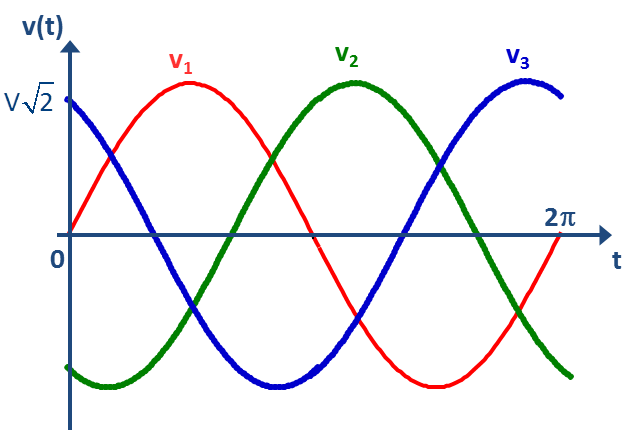
\includegraphics[width=2.84861in,height=1.91389in]{13-MAS-MS/Cours/pandoc/media/image5.png}Distribution en triphasé -- Utilisation des complexes}{Distribution en triphasé -- Utilisation des complexes}}\label{distribution-en-triphasuxe9-utilisation-des-complexes}}

\hypertarget{tensions-simple-et-composuxe9e}{%
\subsubsection{Tensions simple et composée}\label{tensions-simple-et-composuxe9e}}

Une installation \textbf{triphasée} comporte \textbf{3 fils} de ligne identiques appelés \textbf{phases} et parfois un quatrième fil appelé \textbf{neutre}.

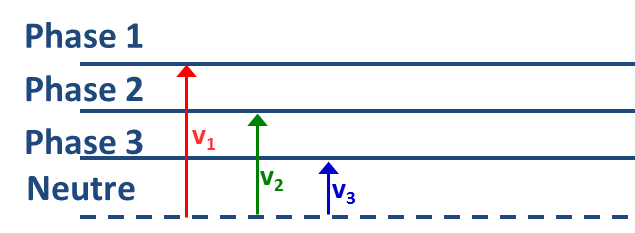
\includegraphics[width=2.83958in,height=1.04167in]{13-MAS-MS/Cours/pandoc/media/image6.png}

Un système triphasé équilibré de tension (ou de courants) est formé de trois grandeurs sinusoïdales de \textbf{même valeur efficace V}, de \textbf{même fréquence f = ω÷2π}et \textbf{déphasées de 120°}les unes par rapport aux autres.

Le système de tensions triphasé le plus utilisé est le \textbf{système direct} dont les expressions temporelles sont :

\begin{quote}
\(v_{1}(t) = V\sqrt{2}\sin(\omega t)\) \(v_{2}(t) = V\sqrt{2}\sin\left( \omega t - \frac{2\pi}{3} \right)\) \(v_{3}(t) = V\sqrt{2}\sin\left( \omega t - \frac{4\pi}{3} \right)\)
\end{quote}

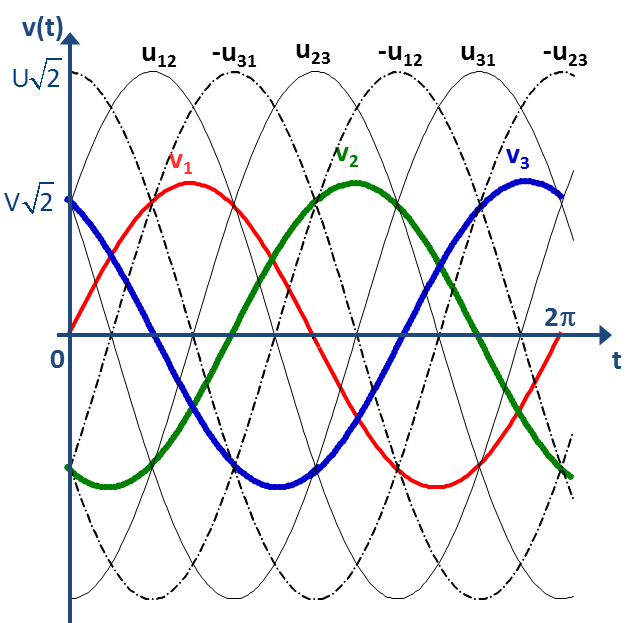
\includegraphics[width=2.83889in,height=2.76319in]{13-MAS-MS/Cours/pandoc/media/image7.png}Un système triphasé est \textbf{équilibré} si:v\textsubscript{1}+v\textsubscript{2}+v\textsubscript{3} =0

La \textbf{tension simple} v\textsubscript{i} est la différence de potentiel entre la \textbf{phase i et le neutre}. Sa valeur efficace est notée V.

La \textbf{tension composée}u\textsubscript{ij} = v\textsubscript{i}-v\textsubscript{j} est la différence de potentiel entre la \textbf{phase i et la phase j}. Sa valeur efficace est notée U.


\includegraphics{13-MAS-MS/Cours/pandoc/media/image8.wmf}

Lorsqu'on parle de réseau triphasé 400 V, c'est la tension composée qui est donnée. La tension simple est donc de 230 V.

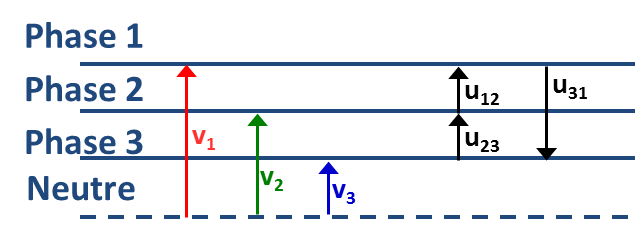
\includegraphics[width=2.90552in,height=1.06604in]{13-MAS-MS/Cours/pandoc/media/image9.png}

\hypertarget{section}{%
\subsubsection*{}\label{section}}
\addcontentsline{toc}{subsubsection}{}

\hypertarget{repruxe9sentation-vectorielle-dun-signal-sinusouxefdal}{%
\subsubsection{Représentation vectorielle d'un signal sinusoïdal}\label{repruxe9sentation-vectorielle-dun-signal-sinusouxefdal}}

Une \textbf{fonction sinusoïdale} peut être représentée par un \textbf{vecteur, tournant à la vitesse} \(\mathbf{\omega}\), dans le plan complexe et dont la \textbf{norme est l'amplitude crête Ŝ}.

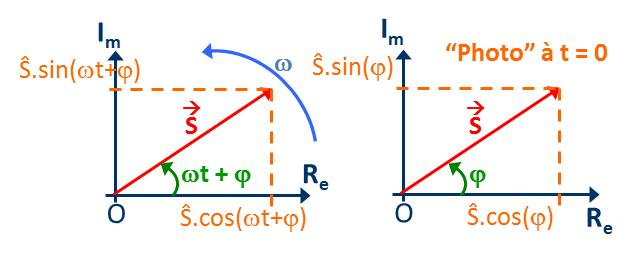
\includegraphics[width=3.68868in,height=1.46514in]{13-MAS-MS/Cours/pandoc/media/image10.jpeg}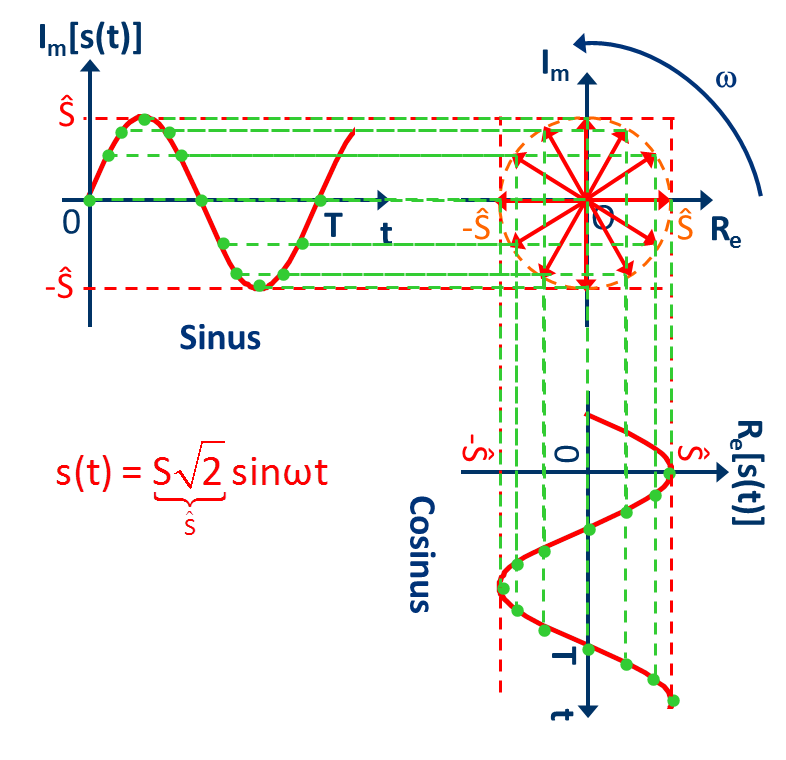
\includegraphics[width=3.57986in,height=3.46181in]{13-MAS-MS/Cours/pandoc/media/image11.png}Les vecteurs représentant une grandeur sinusoïdale sont tous représentés au même instant comme si on avait pris une photo. On les \textbf{représente donc tous à t = 0}.

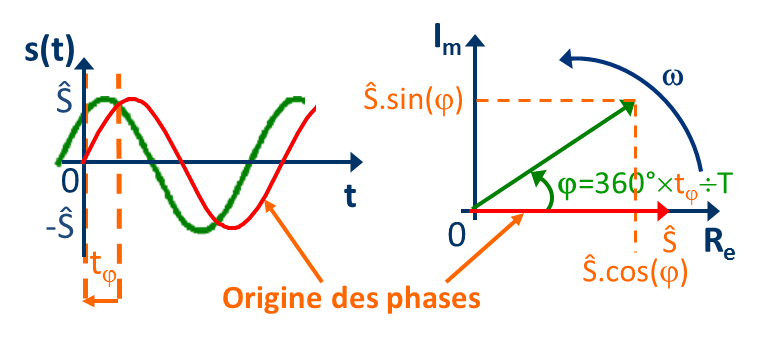
\includegraphics[width=3.05625in,height=1.28264in]{13-MAS-MS/Cours/pandoc/media/image12.png}

Tous les vecteurs seront représentés à partir d'une grandeur qui sera prise \textbf{comme référence (ou origine des phases) et à partir de laquelle seront définis les déphasages.}

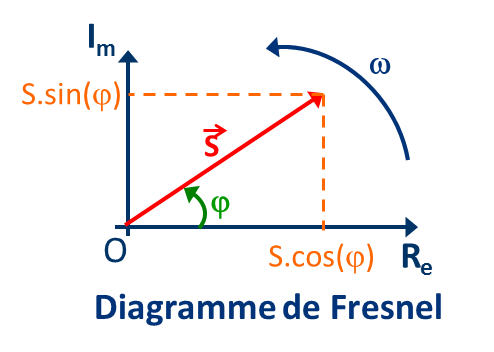
\includegraphics[width=2.075in,height=1.47778in]{13-MAS-MS/Cours/pandoc/media/image13.png}La \textbf{représentation de Fresnel} utilise la \textbf{valeur efficace S} plutôt que l'amplitude (Ŝ = S.√2) car elle est facilement \textbf{mesurable} (multimètre RMS ou ferromagnétique).

Tous les vecteurs seront représentés à partir d'une grandeur qui sera prise \textbf{comme référence (ou origine des phases).}

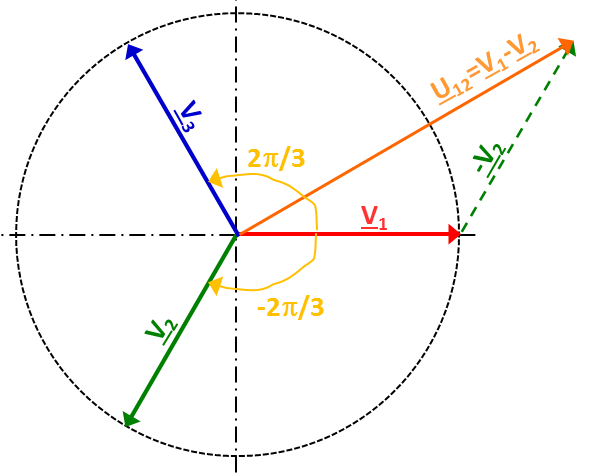
\includegraphics[width=2.61319in,height=2.09861in]{13-MAS-MS/Cours/pandoc/media/image14.png}Le diagramme de Fresnel utilise en fait l'amplitude complexe \ul{S} de s(t) dans un vecteur de \textbf{norme S qui représente la valeur efficace de s(t) et est déphasé d'un angle} \(\mathbf{\varphi\ }\).

La représentation de Fresnel permet de réaliser simplement la somme de fonction sinusoïdale, par construction géométrique. Il suffit alors de remplacer chaque signal par son vecteur de Fresnel équivalent et de réaliser une somme vectorielle.

Dans un système triphasé, la tension v\textsubscript{1} est prise comme référence.

\begin{longtable}[]{@{}
  >{\raggedright\arraybackslash}p{(\columnwidth - 2\tabcolsep) * \real{0.1250}}
  >{\raggedright\arraybackslash}p{(\columnwidth - 2\tabcolsep) * \real{0.8611}}@{}}
\toprule\noalign{}
\begin{minipage}[b]{\linewidth}\raggedright
\begin{quote}
\includegraphics{13-M AS-MS/ Cours/ pandoc /media /image 15.png}\{widt h=``0.6 262696 850393 701in''

height =``0.65 083333 333333 34in''\}
\end{quote}
\end{minipage} & \begin{minipage}[b]{\linewidth}\raggedright
\textbf{Représentation de Fresnel}

\textbf{Représenter} \(\mathbf{V}_{\mathbf{1}}\)\textbf{,} \(\mathbf{V}_{\mathbf{2}}\) \textbf{et} \(\mathbf{V}_{\mathbf{3}}\) \textbf{en prenant} \(\mathbf{V}_{\mathbf{1}}\) \textbf{comme origine des phases.}

\textbf{Construire} \(\mathbf{U}_{\mathbf{31}}\) \textbf{puis donner son expression temporelle}
\end{minipage} \\
\midrule\noalign{}
\endhead
\bottomrule\noalign{}
\endlastfoot
& \\
\end{longtable}

\hypertarget{puissance-ruxe9active}{%
\subsubsection{Puissance réactive}\label{puissance-ruxe9active}}

Nous le verrons plus tard dans le cours mais la machine synchrone peut se comporter comme un récepteur inductif ou capacitif suivant l'excitation de la machine. Lorsque le comportement est capacitif, la machine synchrone fournit de la puissance réactive et porte le nom de compensateur synchrone. Cela été recherché il y a quelques années pour améliorer le facteur de puissance d'une installation électrique. Cette détermination de puissance réactive est donc parfois importante.

Il faut retenir~:

\begin{longtable}[]{@{}
  >{\raggedright\arraybackslash}p{(\columnwidth - 4\tabcolsep) * \real{0.3194}}
  >{\raggedright\arraybackslash}p{(\columnwidth - 4\tabcolsep) * \real{0.3194}}
  >{\raggedright\arraybackslash}p{(\columnwidth - 4\tabcolsep) * \real{0.3333}}@{}}
\toprule\noalign{}
\begin{minipage}[b]{\linewidth}\raggedright
\textbf{Comportement réisistif}

\textbf{(}\(\m athbf{\varphi = 0)}\)
\end{minipage} & \begin{minipage}[b]{\linewidth}\raggedright
\textbf{Comportement inductif}

\textbf{(}\(\mathbf{0  < \varphi \leq}\fra c{\mathbf{\ \pi}}{\m athbf{2}}\mathbf{)}\)
\end{minipage} & \begin{minipage}[b]{\linewidth}\raggedright
\textbf{Comportement capacitif}

\textbf{(}\(\mathbf {-}\frac{\mathbf{\ \p i}}{\mathbf{2}}\mathb f{\leq \varphi < 0)}\)
\end{minipage} \\
\midrule\noalign{}
\endhead
\bottomrule\noalign{}
\endlastfoot
Q = 0 & Q \textgreater{} 0 & Q \textless{} 0 \\
\end{longtable}

Et quelques petites méthodes rapides pour déterminer les puissances réactives pour les dipôles de base.

\begin{longtable}[]{@{}
  >{\raggedright\arraybackslash}p{(\columnwidth - 4\tabcolsep) * \real{0.2555}}
  >{\raggedright\arraybackslash}p{(\columnwidth - 4\tabcolsep) * \real{0.3504}}
  >{\raggedright\arraybackslash}p{(\columnwidth - 4\tabcolsep) * \real{0.3796}}@{}}
\toprule\noalign{}
\begin{minipage}[b]{\linewidth}\raggedright
\textbf{Résistance R}
\end{minipage} & \begin{minipage}[b]{\linewidth}\raggedright
\textbf{Inductance L}
\end{minipage} & \begin{minipage}[b]{\linewidth}\raggedright
\textbf{Condensateur C}
\end{minipage} \\
\midrule\noalign{}
\endhead
\bottomrule\noalign{}
\endlastfoot
\(P = RI^{2} = \frac{U^{2}}{R}\) & \(P = 0\) & \(P = 0\) \\
\(Q = 0\) & \(Q = L\omega I^{2} = \frac{U^{2}}{L\omega}\) & \(Q = - C\omega U^{2} = - \frac{I^{2}}{C\omega}\) \\
\end{longtable}

\begin{longtable}[]{@{}
  >{\raggedright\arraybackslash}p{(\columnwidth - 2\tabcolsep) * \real{0.1250}}
  >{\raggedright\arraybackslash}p{(\columnwidth - 2\tabcolsep) * \real{0.8611}}@{}}
\toprule\noalign{}
\begin{minipage}[b]{\linewidth}\raggedright
\begin{quote}
\includegraphics{13-M AS-MS/ Cours/ pandoc /media /image 15.png}\{widt h=``0.6 262696 850393 701in''

height =``0.65 083333 333333 34in''\}
\end{quote}
\end{minipage} & \begin{minipage}[b]{\linewidth}\raggedright
\textbf{Puissances en triphasé}


\includegraphics{13-MAS-MS/Cours/pandoc/media/image16.emf}

Un réseau triphasé 230 V - 400 V - 50 Hz alimente un récepteur triphasé (R = 20 \(\Omega\) et L = 1 H) tel que~:

\textbf{Déterminer~:}

\textbf{- \ul{Z} puis Z :}

\textbf{- I :}

\textbf{- P :}

\textbf{- Q :}

\textbf{- S :}

\textbf{- cos} \(\mathbf{\varphi}\)\textbf{~:}
\end{minipage} \\
\midrule\noalign{}
\endhead
\bottomrule\noalign{}
\endlastfoot
& \\
\end{longtable}

\hypertarget{onduleur-triphasuxe9}{%
\subsection{Onduleur triphasé}\label{onduleur-triphasuxe9}}

Que ce soit pour la MAS ou la MS, il est nécessaire d'agir sur la fréquence d'alimentation. Pour cela, un \textbf{onduleur triphasé} est utilisé (association de 3 «~bras de ponts~»). Il permet de recréer \textbf{un système triphasé à partir d'une tension continue (appelée aussi «~bus continu~») issue d'une batterie ou à la sortie d'un redresseur}.

La structure est donnée ci-dessous. La charge, modélisée ici par des sources de courants, est le stator d'une MS ou MAS. L'allure de la tension \(v_{c}\) et de son fondamental sont représentés pour la loi de commande MLI classique.

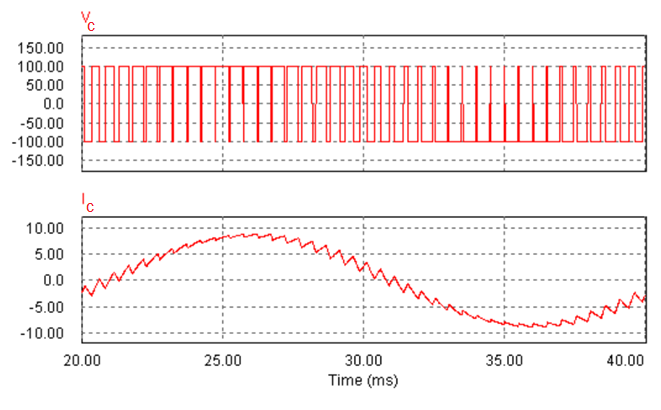
\includegraphics[width=3.72986in,height=2.3125in]{13-MAS-MS/Cours/pandoc/media/image17.png}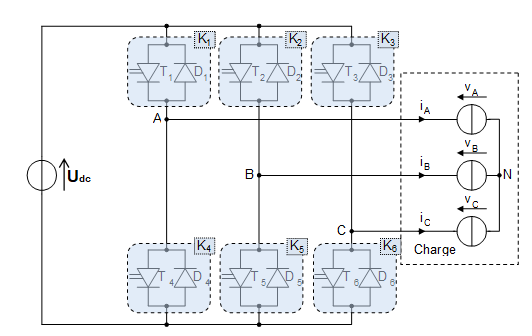
\includegraphics[width=4.4375in,height=2.80208in]{13-MAS-MS/Cours/pandoc/media/image18.png}

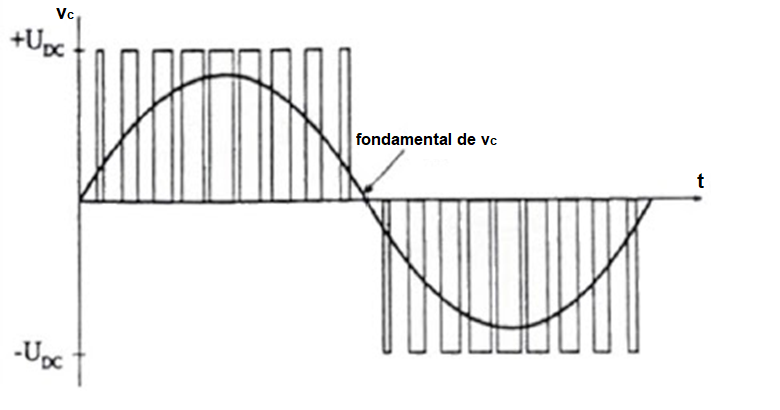
\includegraphics[width=3.88333in,height=2.04167in]{13-MAS-MS/Cours/pandoc/media/image19.png}


\includegraphics[width=4.75in,height=1.96491in]{13-MAS-MS/Cours/pandoc/media/image20.gif}

Cette loi de commande particulière se fait donc avec une génération d'harmonique, qu'une MLI adaptée (sinus-triangle, calculée, vectorielle) permet de limiter en éliminant les harmoniques de basses fréquences. Cela peut être noté sur l'allure du courant \(i_{c}\) représenté ci-dessus, et qui est quasiment sinusoïdal. La machine joue un rôle de filtre passe-bas.

L'intérêt de cette loi de commande est au niveau spectral, si on compare avec une loi de commande qui génère un signal carré et permet de supprimer les harmoniques de rang 3, 5, 7, 9 qui sont les plus contraignants. Les premiers harmoniques avec la MLI précédente sont centrés autour de la fréquence de porteuse.

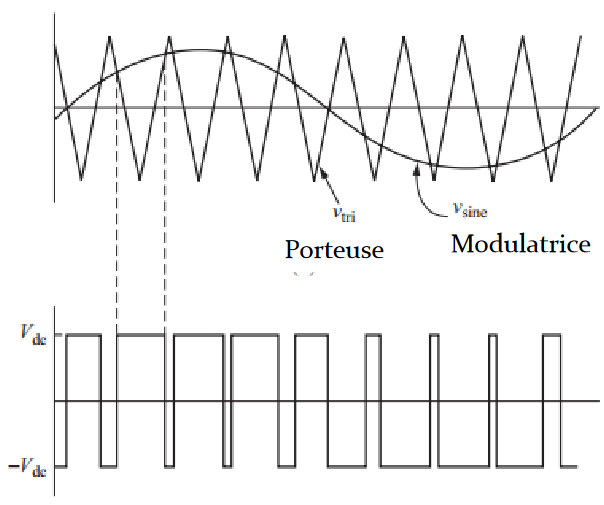
\includegraphics[width=3.22917in,height=2.69988in]{13-MAS-MS/Cours/pandoc/media/image21.png}

Exemple de MLI sinus-triangle~:

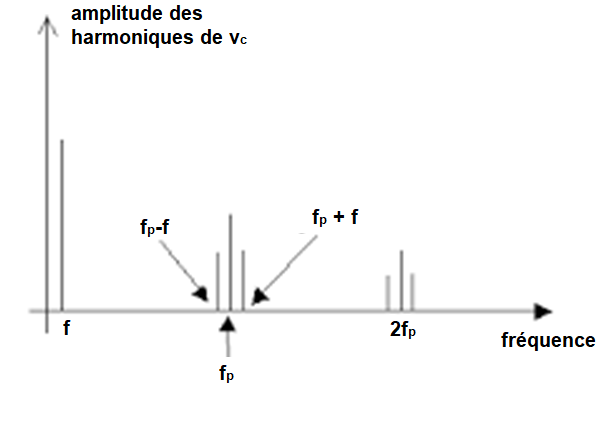
\includegraphics[width=2.91667in,height=2.06301in]{13-MAS-MS/Cours/pandoc/media/image22.png}

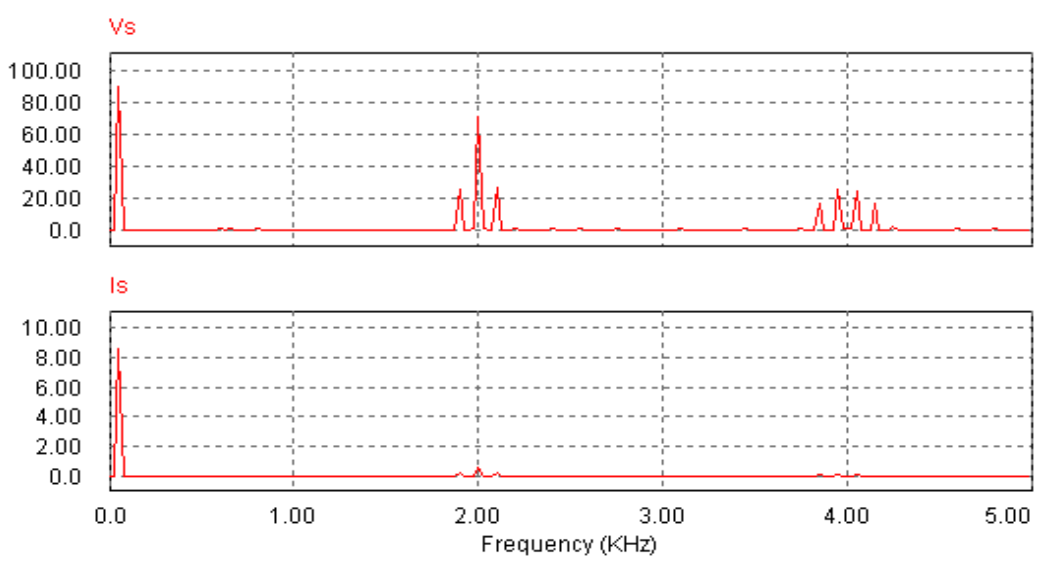
\includegraphics[width=4.77766in,height=2.59747in]{13-MAS-MS/Cours/pandoc/media/image23.png}

On voit que le courant est quasiment sinusoïdal, dû au fait que le moteur agit comme un filtre. La puissance active n'est d'ailleurs transportée que par le fondamental.

\begin{longtable}[]{@{}
  >{\raggedright\arraybackslash}p{(\columnwidth - 2\tabcolsep) * \real{0.1250}}
  >{\raggedright\arraybackslash}p{(\columnwidth - 2\tabcolsep) * \real{0.8611}}@{}}
\toprule\noalign{}
\begin{minipage}[b]{\linewidth}\raggedright
\begin{quote}
\includegraphics{13-M AS-MS/ Cours/ pandoc /media /image 15.png}\{widt h=``0.6 262696 850393 701in''

height =``0.65 083333 333333 34in''\}
\end{quote}
\end{minipage} & \begin{minipage}[b]{\linewidth}\raggedright
\textbf{Onduleur}

La structure de l'onduleur d'une machine synchrone ainsi que la tension v\textsubscript{AN} et l'intensité i\textsubscript{a} du courant absorbé dans la phase «~a~» pour le point de fonctionnement étudié (sur une période entière) sont données ci-dessous~:


\includegraphics[width=2.85069in,height=1.57917in]{13-MAS-MS/C ours/pandoc/media/image24.emf}


\includegraphics[width=4.33194in,height=2.32778in]{13-MAS-MS/ Cours/pandoc/media/image26.emf}

\ul{Etude de l'onduleur}

\textbf{Entourer en rouge un bras d'onduleur.}

\textbf{Expliquer pourquoi il est nécessaire d'avoir une commande complémentaire pour chaque bras~de l'onduleur. Justifier votre réponse.}

\ul{Etude harmonique}


\includegraphics[width=3.55278in,height=2.19861in]{13-MAS-MS/C ours/pandoc/media/image27.emf}Le spectre d'amplitude est donné ci-contre.

\textbf{Quelle est la fréquence du signal v\textsubscript{AN}~?}

\textbf{Quelle est la fréquence de son fondamental v\textsubscript{AN1}~?}

\textbf{Déterminer la valeur efficace du fondamental de la tension, notée V\textsubscript{AN1}~?}

\textbf{Quels sont la fréquence et le rang du premier harmonique non nul de rang strictement supérieur à 1~?}

\textbf{Expliquer qualitativement pourquoi on peut considérer que le courant absorbé par le moteur est sinusoïdal bien que la tension ne le soit pas.}

\ul{Considérations énergétiques}

\textbf{Représenter sur les courbes l'allure du fondamental v\textsubscript{AN1} de la tension v\textsubscript{AN}, en le positionnant correctement en phase et en amplitude.}

\textbf{Déterminer la valeur efficace du courant i\textsubscript{a}, notée I\textsubscript{a} (voir courbe).}

\textbf{Déterminer le déphasage} \(\mathbf{\varphi}_{\mathbf{1}}\) \textbf{entre le courant i\textsubscript{a} et le fondamental de la tension v\textsubscript{AN}.}

\textbf{Déterminer la puissance active P absorbée par la machine triphasé en fonction des notations précédentes. Effectuer l'application numérique.}

\textbf{Déterminer la puissance réactive Q absorbée par la machine triphasée en fonction des notations précédentes. Effectuer l'application numérique.}

\textbf{Peut-on calculer la puissance apparente S~? Quelle donnée manque-t-il~?}
\end{minipage} \\
\midrule\noalign{}
\endhead
\bottomrule\noalign{}
\endlastfoot
& \\
\end{longtable}

\hypertarget{generalites-sur-les-machines-alternatives}{%
\subsection{GENERALITES SUR LES MACHINES ALTERNATIVES}\label{generalites-sur-les-machines-alternatives}}

\hypertarget{px-stator_and_rotor_by_zureksconstitution-dune-machine-triphasuxe9e}{%
\subsubsection[Constitution d'une machine triphasée]{\texorpdfstring{\protect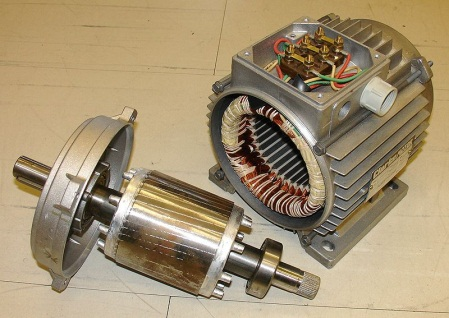
\includegraphics[width=2.04236in,height=1.44722in]{13-MAS-MS/Cours/pandoc/media/image28.jpeg}Constitution d'une machine triphasée}{800px-Stator\_and\_rotor\_by\_ZureksConstitution d'une machine triphasée}}\label{px-stator_and_rotor_by_zureksconstitution-dune-machine-triphasuxe9e}}

La machine triphasée (MAS ou MS), comme toute machine tournante, est constituée~:

\begin{itemize}
\item
  D'un \textbf{stator~:} c'est la partie fixe et qui comporte 3 bobinages \textgreater{} (ou enroulements) alimentés en triphasé.
\item
  D'un \textbf{rotor~:} c'est la partie tournante qui peut comporter soit \textgreater{} des bobinages soit une cage d'écureuil pour une MAS, soit un \textgreater{} aimant permanent ou un rotor bobiné pour une MS.
\item
  D'une plaque à bornes~: fixée sur la carcasse, elle comporte un \textgreater{} ensemble de 6 bornes permettant de connecter les bobines \textgreater{} statoriques à l'alimentation électrique en effectuant le couplage \textgreater{} voulu.
\item
  D'une plaque d'identification (ou plaque signalétique)~: fixée sur \textgreater{} la carcasse, elle représente la fiche d'identité de la machine.
\end{itemize}

\hypertarget{cruxe9ation-du-champ-tournant}{%
\subsubsection{Création du champ tournant}\label{cruxe9ation-du-champ-tournant}}

Le principe de fonctionnement repose sur la création d'un \textbf{champ magnétique statorique tournant}.


\includegraphics[width=3.01667in,height=2.24557in]{13-MAS-MS/Cours/pandoc/media/image29.emf}Le stator est constitué de \textbf{trois bobines décalées dans l'espace de 120° et alimentées par un système triphasé}.

Dans l'expérience suivante, le stator est constitué de trois bobines décalées dans l'espace de 120°. Ces bobines sont alimentées par un système triphasé à fréquence variable obtenu à partir d'un onduleur triphasé de tensions.

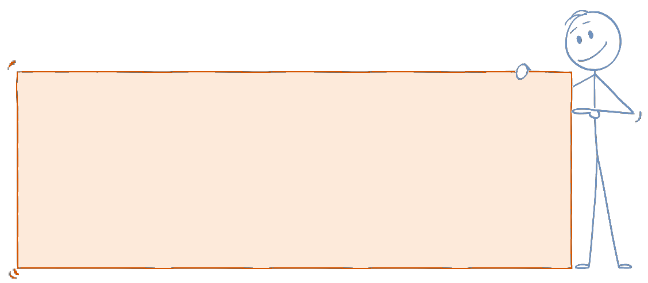
\includegraphics[width=3.54167in,height=1.51667in]{13-MAS-MS/Cours/pandoc/media/image30.png}

\textbf{Champ magnétique pour un enroulement}

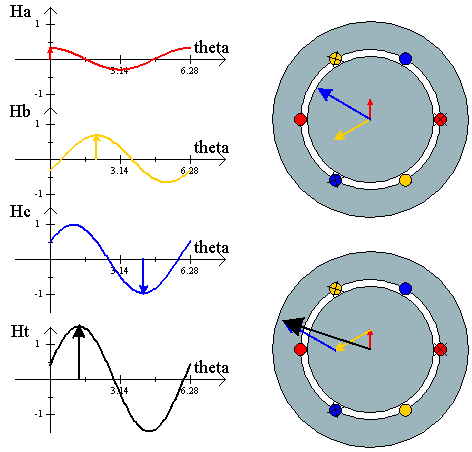
\includegraphics[width=3.70972in,height=3.55208in]{13-MAS-MS/Cours/pandoc/media/image32.png}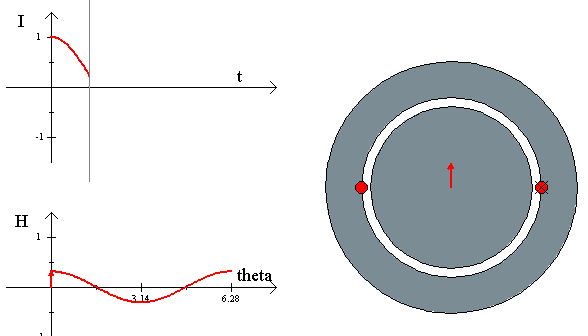
\includegraphics[width=3.19167in,height=1.825in]{13-MAS-MS/Cours/pandoc/media/image33.png}

\textbf{Théorème de Leblanc~:}

Un \emph{courant sinusoïdal} parcourant une \emph{bobine fixe} (à répartition radiale sinusoïdale de courant), peut être remplacé par \emph{deux inducteurs constants} (à répartition radiale sinusoïdale de champ) qui \emph{tournent en sens inverse l\textquotesingle un de l\textquotesingle autre à vitesse constanteΩ=ω/p}, se croisant sur l\textquotesingle axe de la bobine quand le courant dans celle-ci est maximum, et d\textquotesingle amplitude \emph{Φ=Φ\textsubscript{M}/2}.

\textbf{Théorème de Ferraris~:}

Un \emph{système de courants triphasés équilibrés} parcourant un système de \emph{bobines} (à répartition radiale sinusoïdale de courant) \emph{décalées de 120°} l\textquotesingle une de l\textquotesingle autre, peut être remplacé par un \emph{inducteur constant unique} (à répartition radiale sinusoïdale de champ) tournant à vitesse constante \emph{Ω=ω/p} et d\textquotesingle amplitude \emph{Φ=3Φ\textsubscript{M}/2}.

Pour \textbf{une MS}, le rotor tournera à la vitesse du champ tournant, aussi appelée vitesse de synchronisme.

Pour \textbf{une MAS}, les \textbf{bobinages rotoriques étant en court-circuit}, des courants \textbf{induits} sont produits. Ces courants vont à leur tour produire un champ magnétique induit qui va \textbf{s'opposer à la cause qui lui a donné naissance}. Cela se traduit concrètement par un \textbf{phénomène de poursuite du rotor} vis à vis du champ tournant sans qu'il n'arrive jamais à le rattraper. Tant que le rotor a une fréquence de rotation différente que celle du champ inducteur, chaque point de rotor «~voit~» une variation de champ. Les conducteurs rotoriques produisent donc une f.é.m. qui, dans le circuit fermé, va donner naissance à des courants induits.

Le rotor suit donc ce champ magnétique tournant, en tournant à une \textbf{vitesse toujours différente} de celle du champ tournant → \textbf{machine asynchrone}.

\hypertarget{vitesse-de-synchronisme}{%
\subsubsection{Vitesse de synchronisme}\label{vitesse-de-synchronisme}}

Les enroulements statoriques \textbf{alimentés par des courants triphasés de pulsation ω} créent un \textbf{champ magnétique statorique tournant à la vitesse} \(\mathbf{\Omega}_{\mathbf{s}}\) (théorème de Ferraris). Cette vitesse est appelée \textbf{vitesse de synchronisme} et dépend de la pulsation \(\omega\) d'alimentation des courants statoriques et du nombre de paires de pôles des enroulements statoriques.


\includegraphics{13-MAS-MS/Cours/pandoc/media/image34.wmf} 
\includegraphics{13-MAS-MS/Cours/pandoc/media/image35.wmf} ou 
\includegraphics{13-MAS-MS/Cours/pandoc/media/image36.wmf}

\(\Omega_{s}\)~: vitesse de rotation du \textbf{champ tournant}(rad/s)

n\textsubscript{s}~: vitesse de rotation du \textbf{champ tournant}(tr/s) ou Ns (tr/min)

p~: nombre de \textbf{paires de pôles} des enroulements statoriques.

f, \(\omega\)~: \textbf{fréquence et pulsation des courants statoriques}

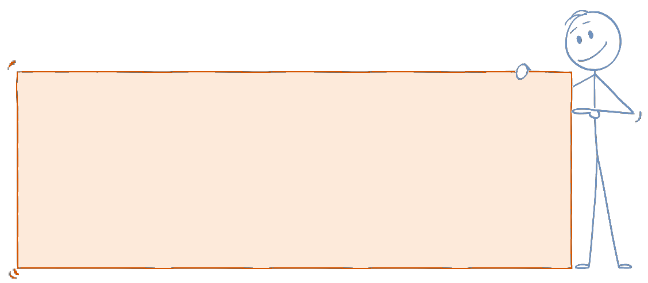
\includegraphics[width=4.575in,height=1.88333in]{13-MAS-MS/Cours/pandoc/media/image30.png}

\begin{longtable}[]{@{}
  >{\raggedright\arraybackslash}p{(\columnwidth - 2\tabcolsep) * \real{0.1250}}
  >{\raggedright\arraybackslash}p{(\columnwidth - 2\tabcolsep) * \real{0.8611}}@{}}
\toprule\noalign{}
\begin{minipage}[b]{\linewidth}\raggedright
\begin{quote}
\includegraphics{13-M AS-MS/ Cours/ pandoc /media /image 15.png}\{widt h=``0.6 262696 850393 701in''

height =``0.65 083333 333333 34in''\}
\end{quote}
\end{minipage} & \begin{minipage}[b]{\linewidth}\raggedright
\textbf{Pôles et vitesse de synchronisme}

\textbf{Donner la vitesse de synchronisme d'une machine tétrapolaire alimentée avec une fréquence de 50Hz.}

\textbf{Donner la vitesse de synchronisme d'une machine bipolaire alimentée avec une fréquence de 100Hz.}

\textbf{Donner le nombre de paires de pôles d'une machine synchrone dont le rotor a vitesse de 2400 tr/min et alimentée avec une fréquence de 80Hz.}

\textbf{Donner le nombre de paires de pôles d'une machine asynchrone dont le rotor a vitesse de 950 tr/min et alimentée avec une fréquence de 50Hz.}
\end{minipage} \\
\midrule\noalign{}
\endhead
\bottomrule\noalign{}
\endlastfoot
& \\
\end{longtable}

\hypertarget{plaque-signaluxe9tique-et-plaque-uxe0-bornes}{%
\subsubsection{Plaque signalétique et plaque à bornes}\label{plaque-signaluxe9tique-et-plaque-uxe0-bornes}}


\includegraphics[width=7.0875in,height=2.79367in]{13-MAS-MS/Cours/pandoc/media/image37.emf}

C'est la carte d'identité de la machine, on y retrouve entre autres :

\textbf{2~:} L'indice de protection IP sur deux chiffres

1\textsuperscript{er} chiffre : protection contre la pénétration des corps solides

2è\textsuperscript{me} chiffre : protection contre la pénétration des corps liquides

\textbf{5~:} Les caractéristiques d'alimentation électrique (ex : 230/400V 9/5,2A 50Hz). Le MAS accepte en général une variation de plus ou moins 10\% autour de ces valeurs nominales.

\textbf{6~:} La puissance utile (on indique toujours ce type de puissance, sauf dans le cas d'une pompe où la puissance absorbée est indiquée) ⇒ puissance mécanique (ex : 2,2kW - 3ch)

RAPPEL~: 1 ch = 736 W en Europe (attention, le cheval britannique est différent car issu du système impérial~: 1HP=746W)

\hypertarget{couplages-uxe9toile-y-triangle-mathbfdelta}{%
\subsubsection{\texorpdfstring{Couplages étoile (Y) / triangle (\(\mathbf{\Delta}\))}{Couplages étoile (Y) / triangle (\textbackslash mathbf\{\textbackslash Delta\})}}\label{couplages-uxe9toile-y-triangle-mathbfdelta}}

Le stator d'une machine asynchrone comporte trois enroulements identiques qui peuvent être raccordés au réseau triphasé (ou couplés) de deux manières différentes~:

\begin{itemize}
\item
  Couplage \textbf{étoile}
\item
  Couplage \textbf{triangle}
\end{itemize}

Le choix du couplage dépend de la machine utilisée et du réseau auquel elle est raccordée.

\begin{longtable}[]{@{}
  >{\raggedright\arraybackslash}p{(\columnwidth - 2\tabcolsep) * \real{0.4861}}
  >{\raggedright\arraybackslash}p{(\columnwidth - 2\tabcolsep) * \real{0.5000}}@{}}
\toprule\noalign{}
\begin{minipage}[b]{\linewidth}\raggedright
\textbf{\ul{Couplage étoile (Y)~:}}

La tension aux bornes d'un enroulement est la \textbf{tension simple} (exemple 230 V).


\includegraphics[width=2.67917in,height=0.96875in]{13-MAS -MS/Cours/pandoc/media/image38.p ng}

En couplage étoile, chaque enroulement de la MAS voit la tension simple et est parcouru par le courant de ligne I.
\end{minipage} & \begin{minipage}[b]{\linewidth}\raggedright
\textbf{\ul{Couplage triangle (∆)~:}}

La tension aux bornes d'un enroulement est la \textbf{tension composée} (exemple 400 V).

\includegraphics[width=2.70278in,height=0.975in]{13- MAS-MS/Cours/pandoc/media/image39 .png}

En couplage triangle, chaque enroulement de la MAS voit la tension composée et est parcouru par un courant \(J = \frac{I}{\sqrt{3}}\)
\end{minipage} \\
\midrule\noalign{}
\endhead
\bottomrule\noalign{}
\endlastfoot
& \\
\end{longtable}

Le choix du couplage dépend~:

\begin{itemize}
\item
  Des tensions du réseau
\item
  Des indications portées sur la plaque signalétique qui donne les \textgreater{} conditions normales de fonctionnement (dites aussi nominales)
\end{itemize}

L'utilisateur choisit le couplage qui convient par l'intermédiaire de la plaque à borne du moteur, qui comporte six bornes auxquelles sont reliées les entrées et les sorties des trois enroulements

\begin{quote}

\includegraphics[width=1.57986in,height=1.0283in]{13-MAS-MS/Cours/pandoc/media/image40.emf}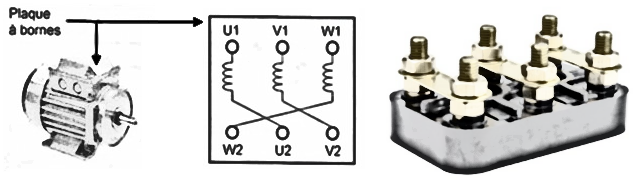
\includegraphics[width=2.74528in,height=1.24275in]{13-MAS-MS/Cours/pandoc/media/image41.png}
\end{quote}

\ul{Normalisation des bornes~:} Entrées U1, V1 et W1, Sorties U2, V2 et W2

\ul{Détermination du couplage~:}

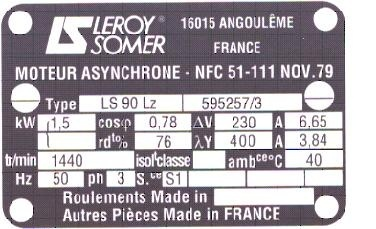
\includegraphics[width=1.87708in,height=1.23611in]{13-MAS-MS/Cours/pandoc/media/image42.jpeg}Sur la plaque à bornes d'une MAS, la plus petite des tensions indiquées est la tension efficace nominale aux bornes d'un enroulement.

\begin{longtable}[]{@{}
  >{\raggedright\arraybackslash}p{(\columnwidth - 8\tabcolsep) * \real{0.1429}}
  >{\raggedright\arraybackslash}p{(\columnwidth - 8\tabcolsep) * \real{0.1648}}
  >{\raggedright\arraybackslash}p{(\columnwidth - 8\tabcolsep) * \real{0.2418}}
  >{\raggedright\arraybackslash}p{(\columnwidth - 8\tabcolsep) * \real{0.2418}}
  >{\raggedright\arraybackslash}p{(\columnwidth - 8\tabcolsep) * \real{0.1868}}@{}}
\toprule\noalign{}
\begin{minipage}[b]{\linewidth}\raggedright
\end{minipage} & \begin{minipage}[b]{\linewidth}\raggedright
\end{minipage} & \begin{minipage}[b]{\linewidth}\raggedright
\textbf{Réseau}
\end{minipage} & \begin{minipage}[b]{\linewidth}\raggedright
\end{minipage} & \begin{minipage}[b]{\linewidth}\raggedright
\end{minipage} \\
\midrule\noalign{}
\endhead
\bottomrule\noalign{}
\endlastfoot
& & \textbf{133/230V} & \textbf{230/400V} & \textbf{400/690V} \\
\textbf{Moteur} & \textbf{133/230V} & \textbf{Y} & \textbf{impossible} & \textbf{impossible} \\
& \textbf{230/400V} & \(\mathbf{\Delta}\) & \textbf{Y} & \textbf{impossible} \\
& \textbf{400/690V} & \textbf{impossible} & \(\mathbf{\Delta}\) & \textbf{Y} \\
\end{longtable}

Si la plus grande tension de la plaque signalétique du moteur correspond à la tension entre phases du réseau (tension composée), on choisit le couplage étoile Y.

On peut retenir «~tensions (réseau et nominale du moteur) égales ⇒ couplage étoile~»

Si la plus petite tension de la plaque signalétique du moteur correspond à la tension entre phases du réseau (tension composée), on choisit le couplage triangle ∆.

On peut retenir «~plus petite tension moteur = plus grande tension réseau⇒ couplage triangle~»

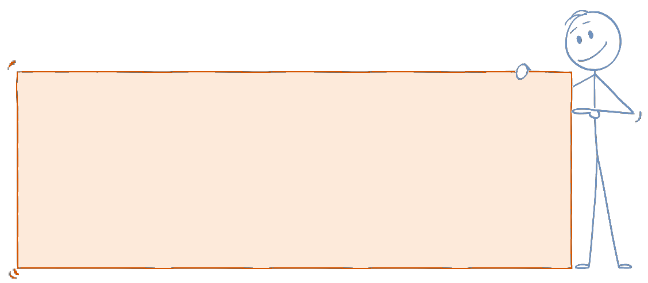
\includegraphics[width=4.575in,height=1.88333in]{13-MAS-MS/Cours/pandoc/media/image30.png}

\begin{longtable}[]{@{}
  >{\raggedright\arraybackslash}p{(\columnwidth - 2\tabcolsep) * \real{0.1250}}
  >{\raggedright\arraybackslash}p{(\columnwidth - 2\tabcolsep) * \real{0.8611}}@{}}
\toprule\noalign{}
\begin{minipage}[b]{\linewidth}\raggedright
\begin{quote}
\includegraphics{13-M AS-MS/ Cours/ pandoc /media /image 15.png}\{widt h=``0.6 262696 850393 701in''

height =``0.65 083333 333333 34in''\}
\end{quote}
\end{minipage} & \begin{minipage}[b]{\linewidth}\raggedright
\textbf{Couplage}

\textbf{Les tensions indiquées sur la plaque signalétique d\textquotesingle un moteur triphasé sont : 400 V / 690 V 50 Hz}

\textbf{\hfill\break
Quel doit être le couplage du moteur sur un réseau triphasé 230 V / 400 V ?}

\textbf{\hfill\break
Et sur un réseau triphasé 400 V / 690 V}\strut
\end{minipage} \\
\midrule\noalign{}
\endhead
\bottomrule\noalign{}
\endlastfoot
& \\
\end{longtable}

\hypertarget{puissances-en-triphasuxe9-uxe9quilibruxe9}{%
\subsubsection{Puissances en triphasé équilibré}\label{puissances-en-triphasuxe9-uxe9quilibruxe9}}

Un récepteur triphasé équilibré peut être considéré comme l'association de 3 récepteurs monophasés identique. L'expression des puissances active, réactive et apparente sont :

\begin{quote}

\includegraphics{13-MAS-MS/Cours/pandoc/media/image43.wmf} 
\includegraphics{13-MAS-MS/Cours/pandoc/media/image44.wmf} 
\includegraphics{13-MAS-MS/Cours/pandoc/media/image45.wmf}
\end{quote}


\includegraphics{13-MAS-MS/Cours/pandoc/media/image46.wmf}\textbf{Théorème de Boucherot~:}

Si un réseau électrique a toutes les grandeurs sinusoïdales de même fréquence, la puissance active (respectivement réactive) totale fournie par le réseau est égale à la somme algébrique des puissances actives (respectivement réactives) consommée par chaque dipôle du réseau.


\includegraphics{13-MAS-MS/Cours/pandoc/media/image47.wmf}\textbf{Facteur de puissance f\textsubscript{p}~:}

Le facteur de puissance est un paramètre qui rend compte de l\textquotesingle efficacité qu\textquotesingle a un dipôle pour consommer de la puissance lorsqu\textquotesingle il est traversé par un courant.

\hypertarget{couple-thermique-equivalent-cth}{%
\subsubsection{\texorpdfstring{Couple Thermique Equivalent (C\textsubscript{th})}{Couple Thermique Equivalent (Cth)}}\label{couple-thermique-equivalent-cth}}

Lorsque le moteur piloté par un variateur développe un couple moteur qui évolue dans le temps de façon cyclique, la détermination du couple nominal du moteur (celui qui conditionne sa capacité et son prix) se fait avec la notion de \textbf{couple thermique équivalent}.

C\textquotesingle est l\textquotesingle échauffement qui limite la capacité d\textquotesingle un moteur à délivrer un couple 24h/24 plus élevé que son couple nominal. Pour un couple moteur égal au couple nominal et développé en permanence, l\textquotesingle équilibre thermique de la machine est assuré. Si le couple délivré est supérieur à la valeur nominale l\textquotesingle échauffement augmente, si le couple délivré est inférieur à la valeur nominale, l\textquotesingle échauffement diminue. On cherche donc à déterminer pour un couple qui évolue dans le temps la valeur du couple qui, développé en permanence (donc sans évolution dans le temps), produirait le même échauffement. Ce couple se nomme couple thermique équivalent C\textsubscript{th}.

On définit le couple thermique équivalent comme la relation \(C_{th}^{2} = \frac{1}{T}.\int_{0}^{T}{C_{i}^{2}(t).dt}\)

En pratique, pour des valeurs constantes de C\textsubscript{i}, on utilisera \(C_{th}^{2} = \frac{1}{T}.\sum_{i}^{}\left( C_{i}^{2} \times t_{i} \right)\)

Pour dimensionner un moteur fonctionnant en régime cyclique, on doit tenir compte du couple dit « thermique équivalent ». Celui-ci doit être \textbf{inférieur ou égal au couple nominal donné par le constructeur}.

\begin{longtable}[]{@{}
  >{\raggedright\arraybackslash}p{(\columnwidth - 2\tabcolsep) * \real{0.1250}}
  >{\raggedright\arraybackslash}p{(\columnwidth - 2\tabcolsep) * \real{0.8611}}@{}}
\toprule\noalign{}
\begin{minipage}[b]{\linewidth}\raggedright
\begin{quote}
\includegraphics{13-M AS-MS/ Cours/ pandoc /media /image 15.png}\{widt h=``0.6 262696 850393 701in''

height =``0.65 083333 333333 34in''\}
\end{quote}
\end{minipage} & \begin{minipage}[b]{\linewidth}\raggedright
\textbf{Cth}

\textbf{Calculer le couple thermique équivalent du moteur à partir du chronogramme suivant.}

\(C_{th}^{2} = \frac{1}{T}\int_{0}^{T}{C_{M}^{2}(t).dt}\)avec T = 0,2 s (5 périodes pour 1 seconde)
\end{minipage} \\
\midrule\noalign{}
\endhead
\bottomrule\noalign{}
\endlastfoot
& \\
\end{longtable}

\begin{longtable}[]{@{}
  >{\raggedright\arraybackslash}p{(\columnwidth - 2\tabcolsep) * \real{0.1250}}
  >{\raggedright\arraybackslash}p{(\columnwidth - 2\tabcolsep) * \real{0.8611}}@{}}
\toprule\noalign{}
\begin{minipage}[b]{\linewidth}\raggedright
\begin{quote}
\includegraphics{13-M AS-MS/ Cours/ pandoc /media /image 15.png}\{widt h=``0.6 262696 850393 701in''

height =``0.65 083333 333333 34in''\}
\end{quote}
\end{minipage} & \begin{minipage}[b]{\linewidth}\raggedright
\textbf{Cth}

\textbf{Calculer le couple thermique équivalent du moteur à partir du chronogramme suivant.}

\begin{quote}

\includegraphics[width=5.52147in,height=3.33605in]{13-MAS-MS/C ours/pandoc/media/image48.png}
\end{quote}
\end{minipage} \\
\midrule\noalign{}
\endhead
\bottomrule\noalign{}
\endlastfoot
& \\
\end{longtable}

\hypertarget{machine-asynchrone-mas}{%
\subsection{Machine Asynchrone (MAS)}\label{machine-asynchrone-mas}}

\hypertarget{glissement}{%
\subsubsection{Glissement}\label{glissement}}

Une des différences entre la MAS et la MS est l'existence d'un glissement pour la MAS. Le glissement traduit le fait que dans une MAS, le rotor ne tourne pas à la vitesse du champ tournant \(\Omega_{s}\). (contrairement à la MS).

Le champ tournant statorique balaie le bobinage rotorique et y induit des forces électromotrices (loi de Lenz). Les bobinages rotoriques étant en court-circuit, des courants induits sont produits. L'action du champ tournant sur ces courants créé un couple électromagnétique.

Le \textbf{rotor} de la MAS \textbf{tourne à une vitesse angulaire} \(\mathbf{\Omega}\mathbf{\ }\)\textbf{inférieure}à la vitesse angulaire du \textbf{champ tournant statorique} \(\mathbf{\Omega}_{\mathbf{s}}\).

Si le rotor tourne à la vitesse du champ tournant, il ne «~voit~» plus de variation de flux et il n'y a plus de fém induite et donc de couple.

Le \textbf{glissement} caractérise la diminution relative de vitesse de rotation. Il est souvent exprimé en \% et dépend du point de fonctionnement de la machine.


\includegraphics{13-MAS-MS/Cours/pandoc/media/image49.wmf}

Le glissement doit être le plus faible possible (plus il sera grand, plus les pertes Joule rotoriques seront grandes).

La fréquence des courants rotoriques induits est fonction du glissement~: 
\includegraphics{13-MAS-MS/Cours/pandoc/media/image50.wmf} 
\includegraphics{13-MAS-MS/Cours/pandoc/media/image51.wmf}

\begin{quote}
f, \(\omega\)~: fréquence et pulsation des courants statoriques

f\textsubscript{R}, \(\omega_{R}\)~: fréquence et pulsation des courants rotoriques

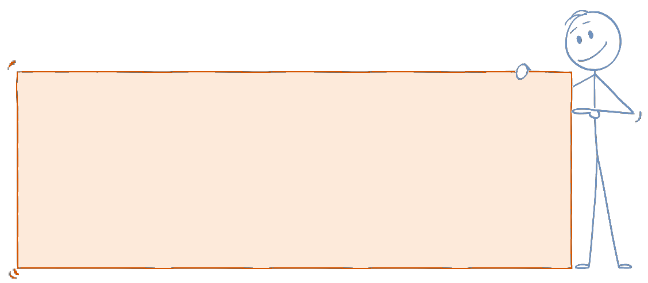
\includegraphics[width=4.575in,height=1.88333in]{13-MAS-MS/Cours/pandoc/media/image30.png}
\end{quote}

\hypertarget{schuxe9ma-monophasuxe9-uxe9quivalent}{%
\subsubsection{Schéma monophasé équivalent}\label{schuxe9ma-monophasuxe9-uxe9quivalent}}

Le schéma équivalent monophasé est une \textbf{représentation mathématique} du fonctionnement en \textbf{régime permanent} de la MAS alimentée par un \textbf{réseau à tension et fréquence constante}.

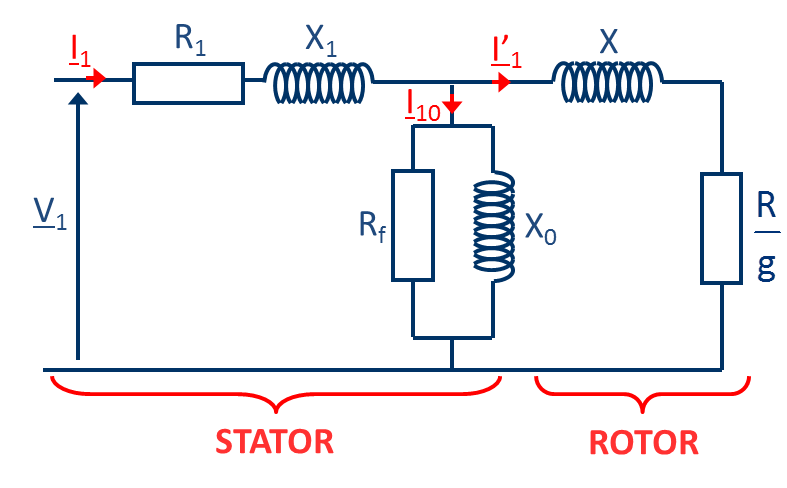
\includegraphics[width=3.54653in,height=2in]{13-MAS-MS/Cours/pandoc/media/image52.png}La résistance R/g n'a aucune signification physique et permet uniquement de représenter la puissance transmise du stator au rotor (P\textsubscript{TR}).

V\textsubscript{1} : tension efficace aux bornes d'une phase du stator

I\textsubscript{1} : courant efficace dans une phase du stator

R\textsubscript{1}: résistance d'une phase du stator

R\textsubscript{f}: résistance modélisant les pertes ferromagnétiques

X\textsubscript{0} : réactance de magnétisation= L\textsubscript{0}ω

X\textsubscript{1} : réactance de fuites au stator= L\textsubscript{1}ω

X : réactance de fuite au rotor ramenée au stator= Lω

R : résistance d'une phase du rotor ramenée au stator

g : glissement

La puissance \textbf{P\textsubscript{TR}} transmise du stator au rotor vaut \(\boxed{P_{TR} = 3.\frac{R}{g}I_{1}'^{2}}\).I'\textsubscript{1} représente la valeur efficace du courant \ul{I'}\textsubscript{1}.

Les pertes fer au stator \textbf{P\textsubscript{fs~}}valent \(\boxed{P_{fs} = 3.\frac{V_{1}^{2}}{R_{f}}}\). V\textsubscript{1} représente la valeur efficace de la tension \ul{V}\textsubscript{1}.

\hypertarget{bilan-de-puissance-et-rendement}{%
\subsubsection{Bilan de puissance et rendement}\label{bilan-de-puissance-et-rendement}}

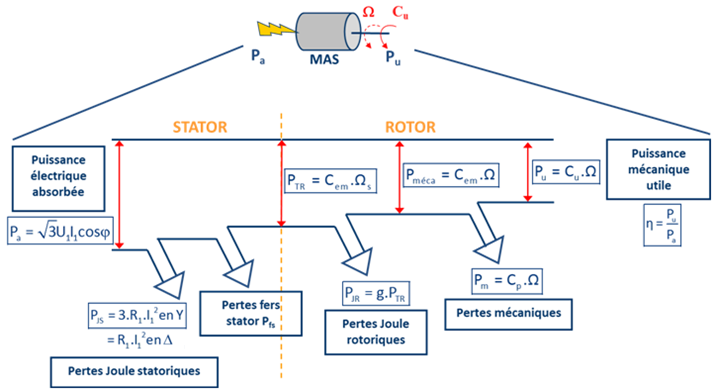
\includegraphics[width=7.06879in,height=3.87806in]{13-MAS-MS/Cours/pandoc/media/image53.png}

\begin{longtable}[]{@{}
  >{\raggedright\arraybackslash}p{(\columnwidth - 2\tabcolsep) * \real{0.1250}}
  >{\raggedright\arraybackslash}p{(\columnwidth - 2\tabcolsep) * \real{0.8611}}@{}}
\toprule\noalign{}
\begin{minipage}[b]{\linewidth}\raggedright
\begin{quote}
\includegraphics{13-M AS-MS/ Cours/ pandoc /media /image 15.png}\{widt h=``0.6 262696 850393 701in''

height =``0.65 083333 333333 34in''\}
\end{quote}
\end{minipage} & \begin{minipage}[b]{\linewidth}\raggedright
\textbf{Etude d'une MAS}

La plaque signalétique de la machine porte les indications suivantes~:

230~V~/~400~V - 50 Hz - 15~kW - 1~440 tr.min\textsuperscript{-1}

La machine est alimentée par un système triphasé équilibré de tensions sinusoïdales de fréquence f~; on note V la valeur efficace des tensions simples et g le glissement.

Dans tout le problème, on néglige les résistances et inductances de fuite statoriques, les pertes fer et les pertes mécaniques.

Sous alimentation nominale, on a obtenu :

- à vide, un courant de ligne d\textquotesingle intensité 6 A.

- à charge nominale, un courant de ligne d\textquotesingle intensité 19,4 A, une puissance absorbée de 11 kW et une fréquence de rotation de 1 440 tr/min.

La machine asynchrone est alimentée sous 220 V/380 V, 50 Hz.

\textbf{Donner le nombre p de paires de pôles de la machine.}

\textbf{Déterminer pour le fonctionnement à charge nominale :}

- le glissement g~:

- la puissance réactive absorbée~:

- le moment du couple nominal C\textsubscript{n}~:

- les pertes rotoriques par effet Joule~:

\textbf{Le schéma équivalent est donné ci-contre, rappeler la signification physique de~:}


\includegraphics[width=1.72014in,height=1.08611in]{13-MAS-MS/C ours/pandoc/media/image54.png}

\begin{itemize}
\item
  L~:
\item
  R~:
\item
  l~:
\end{itemize}

\textbf{Montrer que les éléments du schéma équivalent par phase ont pour valeurs : L = 117 mH l = 9,4 mH r = 0,5 Ω.}
\end{minipage} \\
\midrule\noalign{}
\endhead
\bottomrule\noalign{}
\endlastfoot
& \\
\end{longtable}

\hypertarget{couple-uxe9lectromagnuxe9tique}{%
\subsubsection[Couple électromagnétique]{\texorpdfstring{\protect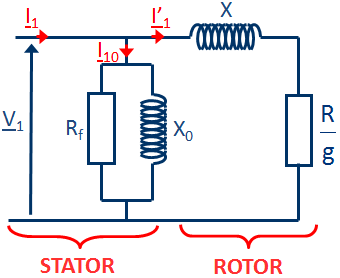
\includegraphics[width=2.56389in,height=2.09375in]{13-MAS-MS/Cours/pandoc/media/image55.png}Couple électromagnétique}{Couple électromagnétique}}\label{couple-uxe9lectromagnuxe9tique}}

Dans la pratique, le schéma monophasé précédent est simplifié en négligeant la chute de tension aux bornes de R\textsubscript{1} et X\textsubscript{1}. Le schéma équivalent simplifié est alors le suivant~:

Les grandeurs étant sinusoïdales on utilise la représentation complexe.

\ul{Z}\textsubscript{1} est l'impédance équivalente à X et R/g en série

\({\overset{\underbar{}}{Z}}_{1} = \frac{{\overset{\underbar{}}{V}}_{1}}{{\underline{I'}}_{1}} = \frac{R}{g} + jX\) \(\Rightarrow \left| {\overset{\underbar{}}{Z}}_{1} \right| = \frac{V_{1}}{I'_{1}} = \sqrt{\left( \frac{R}{g} \right)^{2} + X^{2}} \Rightarrow I'_{1} = \frac{V_{1}}{\sqrt{\left( \frac{R}{g} \right)^{2} + X^{2}}}\)

\(P_{TR} = 3.\frac{R}{g}I_{1}'^{2} = C_{em}.\Omega_{s}\) et \(\Omega_{s} = \frac{\omega}{p}\)

\[\Rightarrow \boxed{C_{em} = \frac{p}{\omega}\frac{3{V_{1}}^{2}\frac{R}{g}}{\left( \frac{R}{g} \right)^{2} + X^{2}} = \frac{3{V_{1}}^{2}}{\Omega_{s}}\frac{Rg}{R^{2} + (Xg)^{2}}}\]

Représentation graphique~:

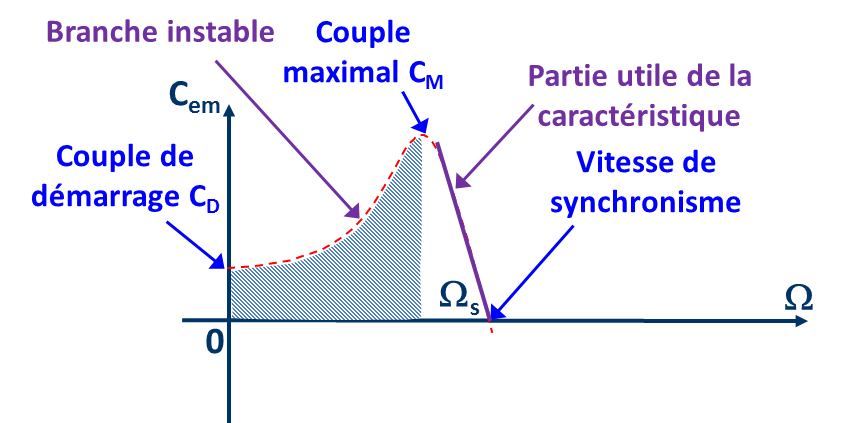
\includegraphics[width=3.60417in,height=1.78264in]{13-MAS-MS/Cours/pandoc/media/image56.png}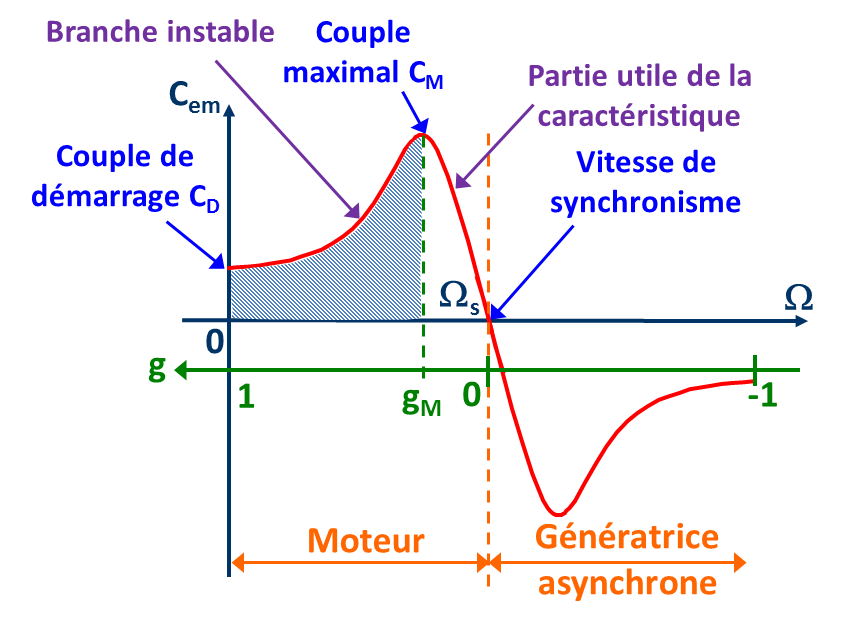
\includegraphics[width=3.21043in,height=2.26389in]{13-MAS-MS/Cours/pandoc/media/image57.png}

\hypertarget{recherche-du-couple-maximal}{%
\subparagraph*{Recherche du couple maximal}\label{recherche-du-couple-maximal}}
\addcontentsline{toc}{subparagraph}{Recherche du couple maximal}

Le couple est maximal lorsque le glissement g vaut une valeur \(\boxed{g_{M} = \frac{R}{X}}\). Le couple est maximal et vaut alors \(C_{em\ max} = C_{M} = \frac{3{V_{1}}^{2}}{\Omega_{s}}\frac{1}{2X}\)

Au démarrage on a g = 1, donc le couple de démarrage s'exprime par \(C_{D} = \frac{3{V_{1}}^{2}}{\Omega_{s}}\frac{R}{R^{2} + X^{2}}\)

Au voisinage du synchronisme, on a g \textless\textless g\textsubscript{M}, on a alors \(C_{em} \approx \frac{3{V_{1}}^{2}}{\Omega_{s}}\frac{g}{R}\)

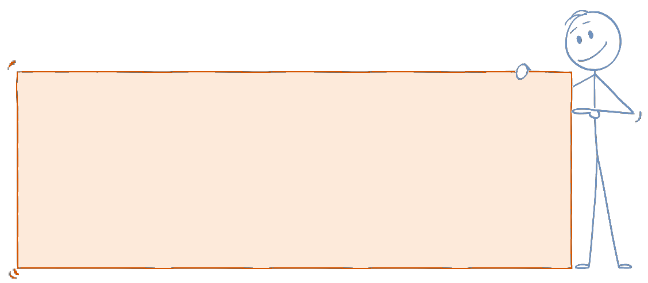
\includegraphics[width=4.575in,height=1.88333in]{13-MAS-MS/Cours/pandoc/media/image30.png}

\begin{longtable}[]{@{}
  >{\raggedright\arraybackslash}p{(\columnwidth - 2\tabcolsep) * \real{0.1250}}
  >{\raggedright\arraybackslash}p{(\columnwidth - 2\tabcolsep) * \real{0.8611}}@{}}
\toprule\noalign{}
\begin{minipage}[b]{\linewidth}\raggedright
\begin{quote}
\includegraphics{13-M AS-MS/ Cours/ pandoc /media /image 15.png}\{widt h=``0.6 262696 850393 701in''

height =``0.65 083333 333333 34in''\}
\end{quote}
\end{minipage} & \begin{minipage}[b]{\linewidth}\raggedright
\textbf{Etude d'une MAS}


\includegraphics[width=1.72014in,height=1.08611in]{13-MAS-MS/C ours/pandoc/media/image54.png}

Le schéma équivalent monophasé d'une MAS est donné ci-contre.

\textbf{Montrer que le moment C du couple de la machine peut s\textquotesingle écrire :}

\(C = \frac{\text{3p}\text{V}^{2}}{\omega} \t imes \frac{\frac{r}{g}}{(\frac{r}{g})^{2} + (l\omega)^{2}}\)

\textbf{Pour quelle valeur de glissement g\textsubscript{max}, le moment du couple est-il maximal ?}

\textbf{Donner la valeur de ce maximum Cmax et la fréquence de rotation correspondante en tr/min.}

\textbf{Tracer l\textquotesingle allure du graphe donnant le moment du couple C en fonction de la fréquence de rotation de 0 à 3000 tr/min sachant que la vitesse de synchronisme est de 1500 tr/min. Préciser le type de fonctionnement suivant la fréquence de rotation.}
\end{minipage} \\
\midrule\noalign{}
\endhead
\bottomrule\noalign{}
\endlastfoot
& \\
\end{longtable}

\hypertarget{variation-de-vitesse-dune-mas}{%
\subsubsection{Variation de vitesse d'une MAS}\label{variation-de-vitesse-dune-mas}}

La vitesse du rotor Ω d'une machine asynchrone est égale à \(\frac{\omega}{p}.(1 - g)\).

Pour faire varier la vitesse, on peut : \(g = \frac{\Omega_{s} - \Omega}{\Omega_{s}} \Rightarrow g.\Omega_{s} = \Omega_{s} - \Omega \Rightarrow \Omega = \Omega_{s}.(1 - g) = \frac{\omega}{p}.(1 - g)\)

\begin{itemize}
\item
  Agir sur le \textbf{glissement g} (avec la tension d'alimentation)
\item
  Agir sur la \textbf{fréquence d'alimentation f}
\item
  Agir que le \textbf{nombre de paires de pôles p}
\end{itemize}

Les méthodes qui n'agissent que sur un seul de ces paramètres ne permettent que de régler la vitesse au détriment du couple et/ou ne permettent pas un réglage continu de la vitesse.

\hypertarget{commande-vf-cte}{%
\subsubsection[Commande V/f = cte~:]{\texorpdfstring{\protect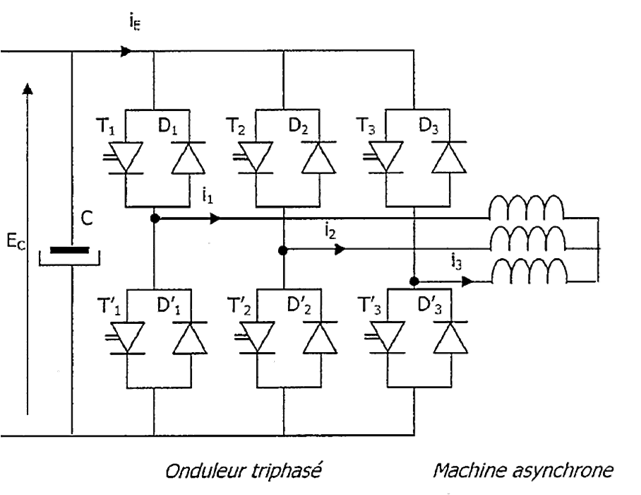
\includegraphics[width=3.50625in,height=2.70694in]{13-MAS-MS/Cours/pandoc/media/image58.png}Commande V/f = cte~:}{Commande V/f = cte~:}}\label{commande-vf-cte}}

Une des méthodes les plus utilisée aujourd'hui est la \textbf{commande V/f=cte} qui permet d'avoir le couple maximal disponible sur toute la gamme de vitesse.

Pour réaliser cette commande, un onduleur de tension est utilisé afin de pouvoir faire varier la fréquence et donc la vitesse de synchronisme.

Lorsqu'on fait varier ce rapport V/f, la caractéristique couple/vitesse «~translate~».

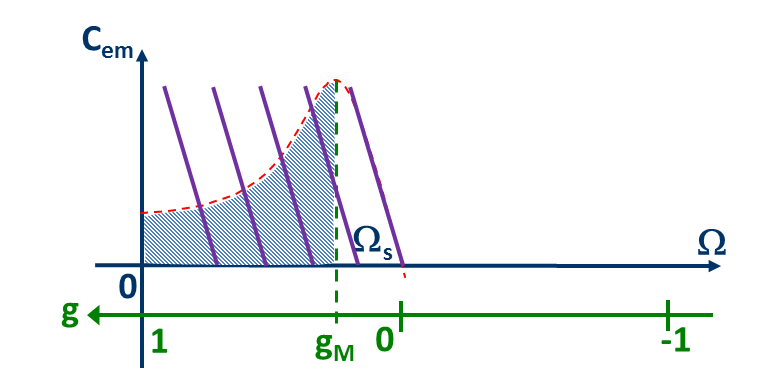
\includegraphics[width=3.2326in,height=1.64151in]{13-MAS-MS/Cours/pandoc/media/image59.png}

En effet, le couple s'écrit dans la zone utile \(C_{em} = - \frac{3p}{4\pi^{2}R}\left( \frac{{V_{1}}^{2}}{f} \right)^{2}\Omega + \frac{3p}{2\pi R}\frac{{V_{1}}^{2}}{f}\)

\begin{longtable}[]{@{}
  >{\raggedright\arraybackslash}p{(\columnwidth - 2\tabcolsep) * \real{0.1250}}
  >{\raggedright\arraybackslash}p{(\columnwidth - 2\tabcolsep) * \real{0.8611}}@{}}
\toprule\noalign{}
\begin{minipage}[b]{\linewidth}\raggedright
\begin{quote}
\includegraphics{13-M AS-MS/ Cours/ pandoc /media /image 15.png}\{widt h=``0.6 262696 850393 701in''

height =``0.65 083333 333333 34in''\}
\end{quote}
\end{minipage} & \begin{minipage}[b]{\linewidth}\raggedright
\textbf{Etude d'une MAS}

La plaque signalétique de la machine porte les indications suivantes~:

230~V~/~400~V - 50 Hz - 15~kW - 1~440 tr.min\textsuperscript{-1}

La machine est alimentée par un système triphasé équilibré de tensions sinusoïdales de fréquence f~; on note V la valeur efficace des tensions simples et g le glissement.

On néglige toute saturation magnétique ainsi que les résistances et inductances de fuite statoriques.

\textbf{Donner le nombre p de paires de pôles de la machine.}

\begin{longtable}[]{@{}
  >{\raggedright\arraybackslash}p{(\columnwidth - 2\tabcolsep) * \real{0.5139}}
  >{\raggedright\arraybackslash}p{(\columnwidth - 2\tabcolsep) * \real{0.2639}}@{}}
\toprule\noalign{}
\endhead
\bottomrule\noalign{}
\endlastfoot
Le schéma équivalent par phase, entre phase et neutre ; il est utilisable quelle que soit la valeur de la tension V.

On a effectué sur la machine les essais suivants à la fréquence f~=~50~Hz~:

- \textbf{Essai n° 1}~: la machine est entraînée à la vitesse de synchronisme~; sous tension V~=~230~V, le courant de ligne a pour intensité efficace I\textsubscript{0}~=~9,5~A et la puissance absorbée est P\textsubscript{0}~=~630~W.

- \textbf{Essai n° 2}~: le rotor de la machine est bloqué~; sous tension V\textsubscript{cc}~=~50~V, le courant de ligne a pour intensité efficace I\textsubscript{cc}~=~30~A et la puissance absorbée est P\textsubscript{cc}~=~830~W. & 
\includegraphics[width=2in,height=\textheight]{13-MAS-M S/Cours/pandoc/m edia/image60.jpe g} \\
\end{longtable}

\textbf{Donner la signification des différents éléments du schéma équivalent.}

\textbf{En utilisant l\textquotesingle essai n° 1, déterminer les valeurs des éléments R et L.}

\textbf{Dans l\textquotesingle essai n°2~:}

\textbf{- Calculer la puissance active consommée par R et la puissance réactive absorbée par L.}

\textbf{- En déduire les puissances actives et réactives absorbées par r et l puis les valeurs des éléments r et l.}

\textbf{Donner l\textquotesingle expression littérale de l\textquotesingle intensité efficace I\textsubscript{2} du courant dans la résistance r/g. En donner une expression approchée si (gl}\(\mathbf{\omega}\)\textbf{)\textsuperscript{2} est négligeable devant r\textsuperscript{2}.}

\textbf{Donner l\textquotesingle expression approchée du moment Ce du couple électromagnétique si (gl}\(\mathbf{\omega}\)\textbf{)\textsuperscript{2} \textless\textless~r\textsuperscript{2}.}

\textbf{Exprimer le glissement g en fonction de la vitesse de rotation N de la machine et de sa fréquence de synchronisme Ns.}

\textbf{En déduire que l\textquotesingle expression approchée du moment Ce du couple électromagnétique peut s\textquotesingle écrire~:}


\includegraphics{13-MAS-MS/Cours/pandoc/media/image61.wmf}

Vérifier que \(A \approx 0,094\) si C\textsubscript{e} est exprimé en N.m, V en volts, f en Hz , ~N\textsubscript{s}~et N~en tr.min\textsuperscript{-1}.

\textbf{Tracer l'allure de la caractéristique approchée Ce = f(N) si V = 230 V et f = 50 Hz pour} \(\mathbf{0 < N < 2}\mathbf{N}_{\mathbf{S}}\)\textbf{. Tracer sur cette courbe, l'allure de la caractéristique réelle. Indiquer les différents modes de fonctionnement. Que se passe-t-il, si on maintient V/f = cte~?}
\end{minipage} \\
\midrule\noalign{}
\endhead
\bottomrule\noalign{}
\endlastfoot
& \\
\end{longtable}

\hypertarget{machine-synchrone}{%
\subsection{MACHINE SYNCHRONE}\label{machine-synchrone}}

Une machine synchrone (MS) est un convertisseur électromécanique réversible. Elle peut fonctionner soit en génératrice (on la nomme alors \textbf{alternateur}), soit en moteur.

Le champ tournant statorique est créé de la même façon que dans la machine asynchrone. Un ensemble d'enroulements alimentés en triphasé qui crée un champ tournant unique à \(\omega_{s}\). Au rotor, on place des aimants (ou des enroulements) dont le champ magnétique va s'accrocher sur le champ tournant statorique.

Le rotor du moteur \textbf{synchrone} tourne à \textbf{la même vitesse} que le champ tournant statorique, \textbf{quelle que soit la charge et la tension d'alimentation}.

\hypertarget{domaines-demploi}{%
\subsubsection{Domaines d'emploi}\label{domaines-demploi}}

\textbf{Petites puissances (de 1 W à 100 W environ)~:}

Entraînement de programmateurs horaires, ventilateurs sur micro-ordinateurs, enregistrement et reproduction audio-vidéo, modélisme (auto, trains et engins volants)

Instrumentation médicale, micro mécanismes automobile, modélisme, mini drone\ldots{}

\textbf{Moyennes puissances (de 100 W à 100 kW environ)~:}

Machines d'usinage numérique (UGV), commande de mécanismes (aéronautique et espace\ldots)

Alternateur automobile classique (1 à 3 kW), entraînement direct du tambour des lave-linge modernes\ldots{}

Motorisation de véhicules électriques ou hybrides (vélo à assistance électrique, scooter, Prius Toyota\ldots)

\textbf{Fortes puissances (de 100 kW à 1,5 GW environ)~:}

Motorisation ferroviaire (TGV atlantique à rotor bobiné 800 kW, 1100kg / TGV sud-est à rotor aimants 722kW, 720kg, 4570tr/min maxi), entrainement d'hélices de bateaux

Production d'énergie électrique, alternateur de centrale nucléaire (900 MW à 1300 MW, 1500 tr/min) ou hydraulique (480 MW, 107 tr/min), éolienne (5 MW)

Industrie : compresseur, centrifugeuse, mélangeuse\ldots{}

\begin{longtable}[]{@{}
  >{\raggedright\arraybackslash}p{(\columnwidth - 4\tabcolsep) * \real{0.3472}}
  >{\raggedright\arraybackslash}p{(\columnwidth - 4\tabcolsep) * \real{0.2917}}
  >{\raggedright\arraybackslash}p{(\columnwidth - 4\tabcolsep) * \real{0.3472}}@{}}
\toprule\noalign{}
\begin{minipage}[b]{\linewidth}\raggedright
\includegraphics{13-MAS-MS/Cou rs/pandoc/media/image6 2.emf}\{width=``2.275in'' height='' 0.9861111111111112in''\}
\end{minipage} & \begin{minipage}[b]{\linewidth}\raggedright
\includegraphics{13-MAS-MS/Cours/ pandoc/media/image 63.emf}
\end{minipage} & \begin{minipage}[b]{\linewidth}\raggedright

\includegraphics{13-M AS-MS/Cours/pandoc/med ia/image64.emf}\{width= ``1.5993055555555555in'' height='' 1.1979166666666667in''\}
\end{minipage} \\
\midrule\noalign{}
\endhead
\bottomrule\noalign{}
\endlastfoot
\begin{minipage}[t]{\linewidth}\raggedright
\begin{longtable}[]{@{}
  >{\raggedright\arraybackslash}p{(\columnwidth - 0\tabcolsep) * \real{0.2778}}@{}}
\toprule\noalign{}
\endhead
\bottomrule\noalign{}
\endlastfoot
\textbf{AR.Drone PARROT quadrirotor}

Moteur brushless spécialement conçu et sa carte de contrôle.

P\textsubscript{u} = 15 W, N variable de 10350 à 41400 tr/min

N = 28000 tr/min en vol stabilisé, soit 3300 tr/min pour les hélices

Contrôle par microcontrôleur basse consommation 8bits. \\
\end{longtable}
\end{minipage} & \textbf{Usinage à grande vitesse (UGV)}

Vitesse de coupe de 1000 m/min dans l'acier, 10 fois la vitesse d'usinage traditionnelle.

Moteur de broche UGV~:

P\textsubscript{u} = 2 kW, N = 40000 tr/min & \textbf{Paquebot de croisière Star Princess}

Propulseur «POD» avec moteur intégré dans une nacelle orientable fixée sous la coque, entraînant une hélice à pas fixe et vitesse variable.

P\textsubscript{umax} = 14 MW à f = 29Hz ; 24 pôles \\
\end{longtable}

\hypertarget{moduxe8le-simplifiuxe9-pour-un-enroulement-ou-phase}{%
\subsubsection{Modèle simplifié pour un enroulement ou phase}\label{moduxe8le-simplifiuxe9-pour-un-enroulement-ou-phase}}

Le schéma monophasé équivalent peut représenter l'alternateur en convention générateur ou le moteur en convention récepteur. Ce modèle est réduit à un \textbf{circuit R, L, E série}~:

\begin{itemize}
\item
  \textbf{E} est la fem développée par la rotation du rotor aux bornes d'un \textgreater{} enroulement. Elle est directement proportionnelle à la vitesse et \textgreater{} au flux φ sous un pôle qui dépend de l'excitation magnétique \textgreater{} fournie par l'inducteur tournant
\item
  \textbf{V} la tension simple aux bornes de l'enroulement et \textbf{I} le \textgreater{} courant le traversant
\item
  \textbf{R\textsubscript{s}} est la résistance d'un enroulement
\item
  \textbf{L\textsubscript{s}} est l'inductance synchrone*. On pose également \textbf{X\textsubscript{s} = \textgreater{} L\textsubscript{s}ω}= réactance de l'enroulement
\end{itemize}

\emph{*Il s'agit d'une inductance qui tient compte du couplage magnétique entre les trois enroulements et le rotor. Elle est valable seulement en régime établi et pour les machines à pôles lisses, d'où une des principales limites du modèle\ldots{}}

\begin{longtable}[]{@{}
  >{\raggedright\arraybackslash}p{(\columnwidth - 2\tabcolsep) * \real{0.4861}}
  >{\raggedright\arraybackslash}p{(\columnwidth - 2\tabcolsep) * \real{0.5000}}@{}}
\toprule\noalign{}
\begin{minipage}[b]{\linewidth}\raggedright
Convention récepteur (moteur)
\end{minipage} & \begin{minipage}[b]{\linewidth}\raggedright
Convention générateur (alternateur)
\end{minipage} \\
\midrule\noalign{}
\endhead
\bottomrule\noalign{}
\endlastfoot
& \\
Couplage électromagnétique en tension~: 
\includegraphics{13-MAS-MS /Cours/pandoc/media/image65.wmf} & \\
Loi des mailles électrique & \\

\includegraphics{13-MAS-MS /Cours/pandoc/media/image66.wmf} & 
\includegraphics{13-MAS-M S/Cours/pandoc/media/image67.wmf} \\
Puissance électrique active (W) appelée ou fournie par la machine~: 
\includegraphics{13-MAS-MS /Cours/pandoc/media/image68.wmf} & \\
Puissance électromagnétique (W)~: 
\includegraphics{13-MAS-MS /Cours/pandoc/media/image69.wmf}

Couple électromagnétique C\textsubscript{em} & \\
\end{longtable}

\hypertarget{diagramme-de-behn-eschenburg}{%
\subsubsection{Diagramme de Behn-Eschenburg}\label{diagramme-de-behn-eschenburg}}

Le diagramme de \textbf{Behn-Eschenburg} est le diagramme de Fresnel correspondant à la loi des mailles électrique~:

\begin{longtable}[]{@{}l@{}}
\toprule\noalign{}
\endhead
\bottomrule\noalign{}
\endlastfoot
Convention récepteur (moteur) Convention générateur (alternateur) \\
\end{longtable}

\begin{center}\rule{0.5\linewidth}{0.5pt}\end{center}

\begin{itemize}
\item
  \textbf{ϕ est le déphasage entre le courant \ul{I} et la tension \textgreater{} \ul{V}}
\item
  \textbf{δ} est l'angle interne, il correspond à l'angle entre \textgreater{} \ul{E} et \ul{V}
\item
  \textbf{ψ est le déphasage entre le courant \ul{I} et la fem \textgreater{} \ul{E}}
\end{itemize}

\hypertarget{diagramme-de-behn-eschenburg-simplifiuxe9}{%
\subsubsection{Diagramme de Behn-Eschenburg simplifié}\label{diagramme-de-behn-eschenburg-simplifiuxe9}}

Dans le tracé du diagramme, la chute de tension dans la résistance \textbf{R\textsubscript{s}} est largement exagérée pour permettre une bonne lisibilité. Dans la réalité, cette résistance est souvent négligée.

Le courant \textbf{\ul{I}} est placé à l'origine des angles. La résistance \textbf{R\textsubscript{s}} est négligée. Le diagramme de Behn-Eschenburg se simplifie alors ainsi~:

\begin{longtable}[]{@{}l@{}}
\toprule\noalign{}
\endhead
\bottomrule\noalign{}
\endlastfoot
Convention récepteur (moteur) Convention générateur (alternateur) \\
\end{longtable}

\begin{center}\rule{0.5\linewidth}{0.5pt}\end{center}

Ainsi le comportement de la machine peut être \textbf{inductif} (courant en retard) ou \textbf{capacitif} (courant en avance) suivant l'excitation de la machine qui règle la valeur de la fém E.

Quand E est supérieur à V, on dit que la machine est surexcitée.

L'angle ψ entre le courant I et la fém E dans l'enroulement est essentiel pour l'expression du couple de la machine et son contrôle.

\hypertarget{relations-de-base}{%
\subsubsection{Relations de base}\label{relations-de-base}}

Les équations fondamentales à connaître pour la machine synchrone sont donc~:

\begin{quote}

\includegraphics{13-MAS-MS/Cours/pandoc/media/image70.wmf}
\end{quote}

\hypertarget{couple-uxe9lectromagnuxe9tique-1}{%
\subsubsection{Couple électromagnétique}\label{couple-uxe9lectromagnuxe9tique-1}}

On détermine le couple électromagnétique à partir de la puissance électromagnétique~:

\begin{quote}

\includegraphics{13-MAS-MS/Cours/pandoc/media/image71.wmf}
\end{quote}

On voit donc qu'à excitation constante, la fém E étant proportionnelle à la vitesse Ω\textsubscript{s}

En instantané, la loi de Faraday donne e = \(\frac{d\varphi}{dt}\), soit en sinusoïdal E = ω.φ = p.Ω\textsubscript{s}.φ = K\textsubscript{e}.Ω\textsubscript{s}

\begin{quote}

\includegraphics{13-MAS-MS/Cours/pandoc/media/image72.wmf} avec K\textsubscript{c} = 3.K\textsubscript{e}
\end{quote}

On retrouve une expression de couple comparable à celui d'une MCC mais dépendant de l'angle ψ.

\hypertarget{autre-expression-du-couple-uxe9lectromagnuxe9tique}{%
\subparagraph*{Autre expression du couple électromagnétique}\label{autre-expression-du-couple-uxe9lectromagnuxe9tique}}
\addcontentsline{toc}{subparagraph}{Autre expression du couple électromagnétique}

Dans le diagramme vectoriel (résistance d'un enroulement négligée), on remarque que E.cosψ = V.cosϕ, ce qui donne les relations P\textsubscript{em} = 3.V.I.cosϕ et \(C_{em} = \frac{P_{em}}{\mathrm{\Omega}_{s}} = \frac{3.V.I.cos\phi}{\mathrm{\Omega}_{s}}\)

\begin{longtable}[]{@{}
  >{\raggedright\arraybackslash}p{(\columnwidth - 2\tabcolsep) * \real{0.1250}}
  >{\raggedright\arraybackslash}p{(\columnwidth - 2\tabcolsep) * \real{0.8611}}@{}}
\toprule\noalign{}
\begin{minipage}[b]{\linewidth}\raggedright
\begin{quote}
\includegraphics{13-M AS-MS/ Cours/ pandoc /media /image 15.png}\{widt h=``0.6 262696 850393 701in''

height =``0.65 083333 333333 34in''\}
\end{quote}
\end{minipage} & \begin{minipage}[b]{\linewidth}\raggedright
\textbf{Etude d'une MS}

Le moteur synchrone est à aimants permanents et possède 8 pôles (p = 4). Les enroulements du stator sont couplés en étoile. L'intensité efficace nominale du courant dans un enroulement est I\textsubscript{N} = 155 A. Afin de simplifier l'étude, les pertes mécaniques ainsi que les pertes fer du moteur synchrone seront négligées.

La machine est étudiée en convention récepteur. Le modèle équivalent à une phase de l'induit est représenté ci-dessous. Les tensions et courants sont supposés sinusoïdaux de pulsation ω = 2πf.

Afin de déterminer les paramètres du modèle, divers essais ont été effectués~:

\begin{itemize}
\item
  Essai n°1~: on a mesuré la résistance entre deux \textgreater{} phases~: r = 0,06 Ω.
\item
  Essai n°2~: sur un banc d'essais, on a entraîné la \textgreater{} machine synchrone à vide par l'intermédiaire d'un \textgreater{} moteur auxiliaire à la vitesse N = 1500 tr/min. On a \textgreater{} mesuré la tension simple aux bornes d'une phase~: 37 \textgreater{} V.
\item
  Essai n°3~: avec une alimentation électrique \textgreater{} appropriée, on a effectué un essai de la machine en \textgreater{} moteur à 1500 tr/min pour lequel ψ = 0°, I = I\textsubscript{max} = \textgreater{} 185 A et V = 49 V.
\item
\end{itemize}

\textbf{Déterminer la fréquence des tensions statoriques si N = 1500 tr/min.}

\textbf{Essai n°1. Déterminer la valeur de la résistance R d'un enroulement.}

\textbf{Essai n°2. On pose E = K.Ω (Ω en rad/s). Déterminer K.}

\textbf{La résistance R n'est pas négligée}

\textbf{A partir du modèle électrique équivalent, écrire la relation entre \ul{V}, \ul{E} et \ul{I}.}

\textbf{Tracer le diagramme vectoriel de cette relation relatif à l'essai n°3. On prendra E comme origine des phases.}

\textbf{En déduire que L = 0,21mH.}

\textbf{La résistance R est négligée.} Pour N = 5000 tr/min, ψ = -59° et I = I\textsubscript{N} = 155 A~:

\textbf{Déterminer f puis ω.}

\textbf{En déduire E = K.Ω et LωI.}

\textbf{Tracer le diagramme vectoriel. On prendra E comme origine des phases. En déduire la valeur de V et celle de ϕ.}
\end{minipage} \\
\midrule\noalign{}
\endhead
\bottomrule\noalign{}
\endlastfoot
& \\
\end{longtable}

\hypertarget{angle-guxe9omuxe9trique-ux3b8}{%
\subsubsection{Angle géométrique θ}\label{angle-guxe9omuxe9trique-ux3b8}}

L'angle ψ est complémentaire de l'angle géométrique θ \((\theta + \psi = \frac{\pi}{2}\ )\) entre l'axe du champ polaire et celui du champ tournant puisque la fem E est en avance de \(\frac{\pi}{2}\) sur le champ (loi de Faraday). Ainsi sinθ = cosψ

Par conséquent, \textbf{l'angle θ représente l'état de charge de la machine ou le couple résistant. Il est nul pour une machine à vide et ne peut pas dépasser 90°, sinon il y a décrochage}. \textbf{La limite de décrochage est donc pour} \(\mathbf{\psi}\mathbf{\leq 0.}\)

\hypertarget{bilan-de-puissances}{%
\subsubsection{Bilan de puissances}\label{bilan-de-puissances}}

Les pertes de la \textbf{machine synchrone triphasée} sont~:

\begin{itemize}
\tightlist
\item
  Des \textbf{pertes joules au stator (induit)} \textbf{P\textsubscript{JS} = 3.R\textsubscript{s}.I²}
\end{itemize}

(R\textsubscript{S} résistance d'un enroulement statorique et I courant dans un enroulement en branchement étoile)

\begin{itemize}
\tightlist
\item
  Des \textbf{pertes mécaniques} \textbf{P\textsubscript{m}}
\end{itemize}

Frottements mécaniques fonction essentiellement de la vitesse de rotation pour les machines usuelles ou du carré de la vitesse à cause des effets aérodynamiques pour les machines ayant une vitesse élevée par exemple broche UGV à N\textsubscript{S} = 20 000 tr/min

\begin{itemize}
\tightlist
\item
  Des \textbf{pertes fer ou magnétiques} \textbf{P\textsubscript{fe}}
\end{itemize}

On regroupe parfois les pertes mécaniques et fer sous le nom de \textbf{pertes collectives} P\textsubscript{c} = P\textsubscript{m} + P\textsubscript{fe}

\begin{itemize}
\tightlist
\item
  Des \textbf{pertes d'excitation} \textbf{P\textsubscript{e} = R\textsubscript{e}.I\textsubscript{e}² = U\textsubscript{e}.I\textsubscript{e}}
\end{itemize}

Si l'inducteur de résistance R\textsubscript{e} est bobiné

\begin{longtable}[]{@{}l@{}}
\toprule\noalign{}
\endhead
\bottomrule\noalign{}
\endlastfoot
Convention récepteur (moteur) Convention générateur (alternateur) \\
\end{longtable}

Rendement\\

\includegraphics{13-MAS-MS/Cours/pandoc/media/image73.wmf}\\
-----------------------------------------------------------------------------------

On trouve aussi la notation P\textsubscript{totale} = P\textsubscript{a} = P\textsubscript{u} + P\textsubscript{J} + P\textsubscript{c}

\hypertarget{expression-du-couple}{%
\subparagraph*{Expression du couple}\label{expression-du-couple}}
\addcontentsline{toc}{subparagraph}{Expression du couple}

Si l'on néglige toutes les pertes, on peut écrire puissance mécanique = puissance électrique

Soit C\textsubscript{u}.Ω\textsubscript{s} = 3.V.I.cosϕ = 3.E.I.cosψ = 3.K\textsubscript{e}.Ω\textsubscript{s}.I.cosψ d'où C\textsubscript{u} = 3.K\textsubscript{e}.I.cosψ = 3.K\textsubscript{e}.I.sinθ avec K\textsubscript{e} = p.φ

Le couple du moteur synchrone est maximum quand l'angle θ vaut π/2

\hypertarget{risque-de-duxe9crochage}{%
\subparagraph*{Risque de décrochage}\label{risque-de-duxe9crochage}}
\addcontentsline{toc}{subparagraph}{Risque de décrochage}

L'angle δ représente l'angle de décalage mécanique entre le rotor et le champ statorique lors d'un fonctionnement moteur. Si cet angle dépasse 90°, le moteur rentre dans une phase instable où le rotor «~décroche~» de l'attraction du champ tournant.

\textbf{La conséquence est que le moteur s'arrête et qu'il faut le redémarrer}. Toutes les commandes qui permettent de faire fonctionner les moteurs synchrones à vitesse variable permettent en réalité d'asservir la position du champ tournant pour que l'angle mécanique reste à une valeur toujours inférieure à 90°. On parle alors de «~machine synchrone auto-pilotée~» ou de «~moteur à courant continu sans balais~» ou «~brushless~».

\hypertarget{variation-de-vitesse-de-la-ms}{%
\subsubsection{Variation de vitesse de la MS}\label{variation-de-vitesse-de-la-ms}}

Dans le cas le plus général, le contrôle de la machine synchrone peut se faire en agissant sur 3 paramètres~:

\begin{itemize}
\item
  La fem \textbf{E} par le courant d'excitation \textbf{I\textsubscript{e}} si la machine est \textgreater{} à inducteur bobiné, en agissant sur la valeur du flux φ sous un \textgreater{} pôle. Ceci est impossible si la machine est à aimants permanents.
\item
  Le courant \textbf{I} dans les phases lorsque la machine est associée à \textgreater{} un convertisseur de puissance avec contrôle de courant (capteur à \textgreater{} effet Hall nécessaire).
\item
  L'angle \textbf{ψ} lorsque la position du rotor est contrôlée par capteur \textgreater{} angulaire (fourche optique, codeur incrémental, synchro-résolver). \textgreater{} L'alimentation des 3 phases est alors coordonnée à l'information \textgreater{} de ce capteur (pilotage des interrupteurs d'un onduleur). Il \textgreater{} s'agit alors d'un \textbf{autopilotage.}
\end{itemize}

Un pilotage complet donne lieu à un ensemble dit «~brushless~» (traduction mot à mot «~sans balais~»), par comparaison à la fonction réalisée par l'ensemble collecteur + balais d'une MCC.

\hypertarget{moteur-brushless-ou-ms-autopilotuxe9e}{%
\subsubsection[Moteur Brushless ou MS autopilotée]{\texorpdfstring{\protect
\includegraphics{13-MAS-MS/Cours/pandoc/media/image74.emf}Moteur Brushless ou MS autopilotée}{Moteur Brushless ou MS autopilotée}}\label{moteur-brushless-ou-ms-autopilotuxe9e}}

L'organisation de la commande de la machine synchrone autopilotée est présentée ci-contre. La commande permet d'imposer l'amplitude du courant \textbf{I\textsubscript{ref}} et l'angle d'autopilotage \textbf{ψ\textsubscript{ref}}.

Afin de maximiser le couple, l'angle d'autopilotage est maintenu à 0 {[}\(\pi\rbrack\) grâce aux capteurs et aux asservissements.

\begin{longtable}[]{@{}
  >{\raggedright\arraybackslash}p{(\columnwidth - 2\tabcolsep) * \real{0.1250}}
  >{\raggedright\arraybackslash}p{(\columnwidth - 2\tabcolsep) * \real{0.8611}}@{}}
\toprule\noalign{}
\begin{minipage}[b]{\linewidth}\raggedright
\begin{quote}
\includegraphics{13-M AS-MS/ Cours/ pandoc /media /image 15.png}\{widt h=``0.6 262696 850393 701in''

height =``0.65 083333 333333 34in''\}
\end{quote}
\end{minipage} & \begin{minipage}[b]{\linewidth}\raggedright
\textbf{Unité de vissage}

La machine est modélisée par le modèle de Behn-Eschenburg, la résistance de chaque phase est négligée. La figure ci-contre présente le schéma équivalent par phase de la machine, ainsi que les conventions utilisées.

Les pertes fer et mécaniques sont supposées négligeables. L'étude est faite en régime établi.

\(\varphi\) : Déphasage entre le courant i\textsubscript{i} et la tension v\textsubscript{i}

ψ : Déphasage entre la fém. \textbf{e\textsubscript{i}} et le courant \textbf{i\textsubscript{i}}

Le constructeur donne~:

\begin{itemize}
\item
  le nombre de paires de pôles~: p = 3~;
\item
  l'inductance cyclique~: L = 7,5 mH~;
\item
  la constante de fem~(
\includegraphics{13-MAS-MS/Cours/pandoc/media/image75.wmf})~: K = 0,13 V/(rad/s).
\end{itemize}

\textbf{Calculer la pulsation} \(\mathbf{\omega}\) \textbf{et la fréquence f des grandeurs statoriques si la machine tourne à 3600 tr/min.}

\textbf{Montrer que le couple fourni par la machine peut se mettre sous la forme} \(\mathbf{C}\mathbf{=}\mathbf{K}_{\mathbf{c}}\
mathbf{.}\mathbf{I}\mathbf{.}\mathbf{\cos}\mathbf{\psi}\)\textbf{. Déterminer} \(\mathbf{K}_{\mathbf{c}}\)\textbf{.}

\textbf{Pour un couple et une vitesse donnée, quel angle d'autopilotage ψ permet de minimiser les courants dans les bobinages de la machine en fonctionnement frein puis moteur ?}

\textbf{Calculer la puissance absorbée par la machine. Quelle est la condition sur} \(\mathbf{\varphi}\) \textbf{pour obtenir un fonctionnement moteur puis frein~?}

\textbf{Tracer l'allure des diagrammes vectoriels de Behn Eschenburg en fonctionnement moteur puis en fonctionnement frein. On prendra la phase de E comme origine et on supposera que} \$ \left\textbar{} \mathbf{\cos}\mathbf{\psi} \right\textbar{}\mathbf{= 1}\$\textbf{.}

\textbf{Pour le fonctionnement moteur et pour N = 3 000 tr/min et I = 6,7 A, déterminer~:}

\textbf{- le facteur de p uissance~cos}\(\mathbf{\ }\mathbf{\varphi}\mathbf{\ }\)\textbf{;}

\textbf{- la tension simple efficace V,}

\textbf{- le couple C.}
\end{minipage} \\
\midrule\noalign{}
\endhead
\bottomrule\noalign{}
\endlastfoot
& \\
\end{longtable}

\hypertarget{sources}{%
\subsection{Sources}\label{sources}}

Ce cours a été élaboré à l'aide de nombreuses ressources~provenant de différents collègues~de l'UPSTI.\\

\hypertarget{exercices-du-chapitre}{%
\subsection{Exercices du chapitre}\label{exercices-du-chapitre}}


\includegraphics[width=5.46667in,height=8.37353in]{13-MAS-MS/Cours/pandoc/media/image76.png}


\includegraphics[width=1.35556in,height=0.38889in]{13-MAS-MS/Cours/pandoc/media/image77.png} 
\includegraphics[width=0.89057in,height=0.5566in]{13-MAS-MS/Cours/pandoc/media/image78.png}\textbf{BANC BALAFRE}

\emph{(\ul{Source} : ATS 2019)}

\textbf{Mise en situation}

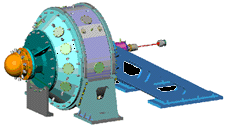
\includegraphics[width=2.36806in,height=1.32083in]{13-MAS-MS/Cours/pandoc/media/image79.png}Le banc BALAFRE (BAnc d\textquotesingle essais à LAmes Fluides à haut REynolds) est un banc d\textquotesingle essai destiné à l\textquotesingle identification du comportement des étanchéités du type joint annulaire. Il est dimensionné pour l\textquotesingle étude de joints utilisés dans des turbomachines que l\textquotesingle on trouve dans les domaines du spatial et de l\textquotesingle énergie.

Le banc BALAFRE a été développé par la société CSTM (Conception de Systèmes et Technologie Mécanique) en collaboration avec l\textquotesingle institut Pprime de l\textquotesingle université de Poitiers.

\textbf{\ul{Principe de fonctionnement du banc~:}}

Le joint que l\textquotesingle on souhaite caractériser est monté sur les pièces joint (rotor) et joint (stator). Pour obtenir un comportement représentatif du fonctionnement réel du joint, on injecte de l\textquotesingle eau sous-pression à l\textquotesingle entrée du banc. Cette eau circule entre le stator et le rotor, en formant un film liquide. Le comportement dynamique de ce film liquide dépend des propriétés du joint. C\textquotesingle est ce comportement (exprimé sous la forme de matrices de raideur, d\textquotesingle amortissement et de masse) que l\textquotesingle on cherche à caractériser.

Pour effectuer cette identification, il est donc nécessaire~:

\begin{itemize}
\item
  d\textquotesingle entraîner le rotor en rotation
\item
  de provoquer une perturbation du film liquide.
\end{itemize}

Un moteur asynchrone triphasé Leroy Sommer PLS- 280-MP est utilisé pour entraîner le rotor. Pendant un essai, le rotor doit avoir une vitesse stabilisée à 6000 tr.min\textsuperscript{-1}.

La perturbation du film liquide est générée par huit actionneurs piézoélectriques et transmise au cœur de butée double.

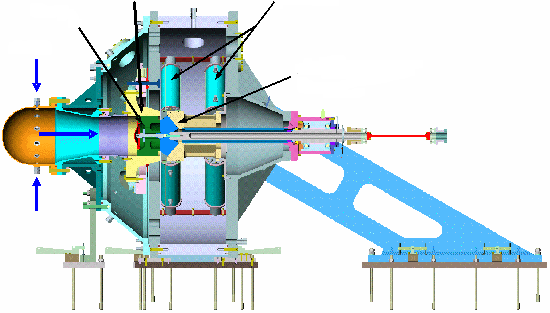
\includegraphics[width=5.70232in,height=3.24514in]{13-MAS-MS/Cours/pandoc/media/image80.png}

\textbf{\ul{Données et hypothèses~:}}

\begin{itemize}
\item
  Le couple résistant exercé par le film d\textquotesingle eau sur le joint (rotor) à \textgreater{} 6000 tr.min\textsuperscript{-1} est estimé à C\textsubscript{res} = 300 N.m
\item
  La vitesse cible N\textsubscript{c} (vitesse de rotation du rotor de joint) doit \textgreater{} pouvoir être réglée à une valeur choisie entre 5000 et 7000 \textgreater{} tr.min\textsuperscript{-1}
\item
  La mise en rotation doit se faire à accélération constante pendant \textgreater{} une durée n\textquotesingle excédant par T\textsubscript{acc} = 5 s
\item
  Le réseau d\textquotesingle alimentation électrique fournit une tension 230/ 400 V \textgreater{} en 50 Hz
\item
  La plaque signalétique du moteur est reproduite ci-contre
\item
  Les pertes Joules statoriques, les pertes fer et les pertes \textgreater{} mécaniques dans le moteur sont négligées
\end{itemize}

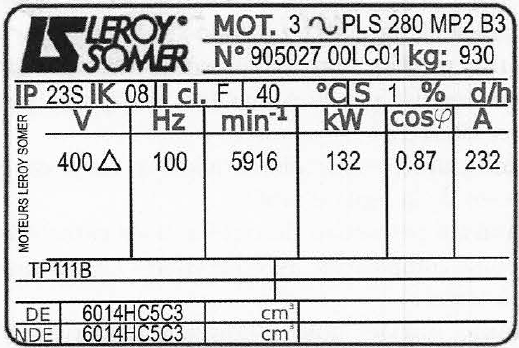
\includegraphics[width=3.13681in,height=2.10347in]{13-MAS-MS/Cours/pandoc/media/image81.png}

\textbf{Modélisation de la motorisation}

\textbf{1.} En utilisant les informations de la plaque signalétique, \textbf{déterminer}~:

\begin{itemize}
\item
  Le couplage du moteur et la valeur nominale de la tension U\textsubscript{s}, \textgreater{} définie sur le schéma électrique équivalent
\item
  Le nombre de paires de pôles p
\item
  Le glissement nominal g\textsubscript{N}
\item
  Le couple utile nominal C\textsubscript{uN}
\end{itemize}

On donne sur la figure ci-contre le modèle équivalent ramené au stator d'une phase du moteur. L\textsubscript{0} représente l\textquotesingle inductance de magnétisation et L\textsubscript{c} l\textquotesingle inductance des fuites totales d\textquotesingle une phase (rotorique ramenée au stator et stator). On note g le glissement.

On rappelle que la puissance dissipée dans la résistance \(\frac{R}{g}\) correspond à la puissance transmise du stator au rotor. Cette puissance peut être décomposée en une résistance R correspondant aux pertes Joule dans le rotor en série avec une résistance \(\frac{R(1 - g)}{g}\) correspondant à la puissance électromécanique fournie au rotor.

\textbf{2.} \textbf{Exprimer} le couple électromagnétique C\textsubscript{EM} en fonction de \(U_{s}^{2}\), ω (pulsation d'alimentation du moteur), g, R, L\textsubscript{c} et p. \textbf{En déduire} que l'expression du couple utile disponible sur l'arbre moteur est \(C_{u} = \frac{3pU_{s}^{2}}{\omega}.\frac{\frac{R}{g}}{\left( \frac{R}{g} \right)^{2} + \left( L_{c}\omega \right)^{2}}\)

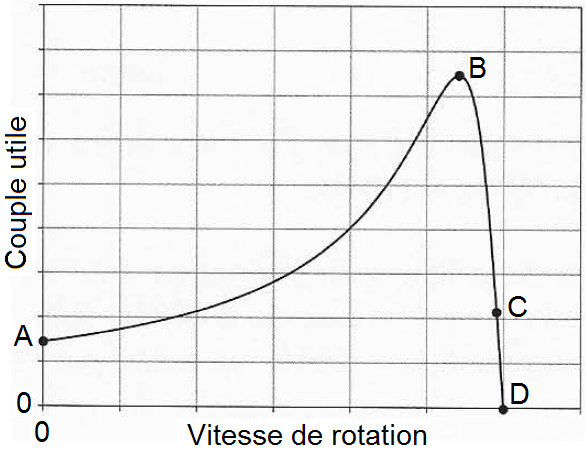
\includegraphics[width=2.87708in,height=2.20694in]{13-MAS-MS/Cours/pandoc/media/image82.png}À l\textquotesingle aide de cette équation, on obtient l\textquotesingle allure de la courbe de couple en fonction de la vitesse de rotation N de l\textquotesingle arbre moteur.

\textbf{3.} À l\textquotesingle aide des points A, B, Cet D, \textbf{identifier} sur cette courbe~:

\begin{itemize}
\item
  Le point de fonctionnement nominal
\item
  Le démarrage du moteur
\item
  Le point de synchronisme
\item
  La zone de fonctionnement instable du moteur
\end{itemize}

\textbf{4.} \textbf{Déterminer} l'expression du couple utile maximal C\textsubscript{M} pour une valeur du glissement g\textsubscript{M}.

Le constructeur précise le rapport du couple maximal sur le couple nominal \(\frac{C_{M}}{C_{N}} = 3,5\).

\textbf{5.} \textbf{En déduire} l\textquotesingle expression de L\textsubscript{c} en fonction de p, U\textsubscript{s}, C\textsubscript{M} et ω. \textbf{Faire} l\textquotesingle application numérique.

\textbf{6.} Que peut-on dire de \(\frac{R}{g}\) par rapport à L\textsubscript{c}ω au voisinage du point de fonctionnement nominal~? \textbf{En déduire} l\textquotesingle expression de R en fonction du couple nominal C\textsubscript{N}, du glissement nominal g\textsubscript{N}, de p, U\textsubscript{s} et de ω. \textbf{Faire} l'application numérique.

Le variateur utilisé pour la commande du moteur fonctionne en \(\frac{U_{s}}{f}\) constant. À l\textquotesingle aide des valeurs calculées précédemment, on a tracé les courbes de couple utile en fonction de la vitesse de rotation pour différentes valeurs de fréquence de commande.

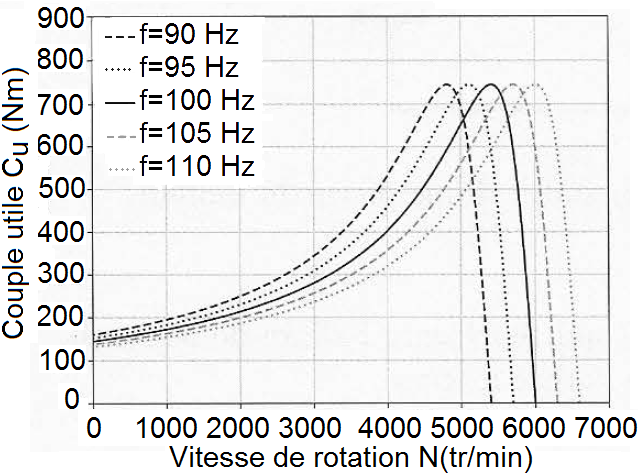
\includegraphics[width=2.93396in,height=2.17961in]{13-MAS-MS/Cours/pandoc/media/image83.png} 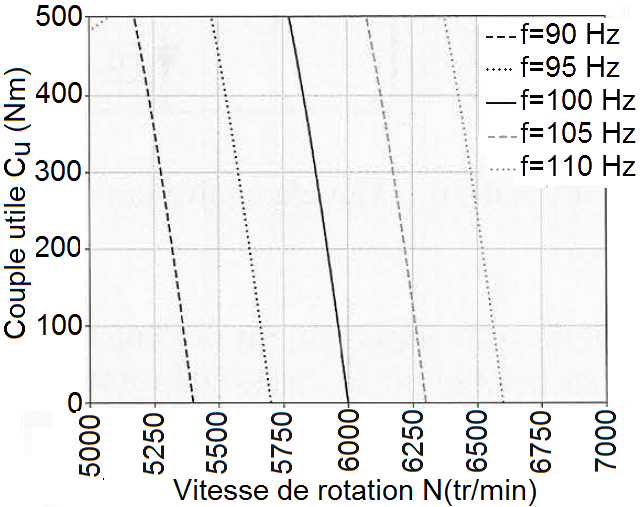
\includegraphics[width=2.93396in,height=2.32395in]{13-MAS-MS/Cours/pandoc/media/image84.png}

Courbe complète Zoom sur la partie utile

Évolution du couple utile en fonction de la vitesse de rotation pour des fréquences de commande de 90 à 110 Hz

\textbf{7.} À l'aide de ces courbes, \textbf{déterminer} quelle fréquence doit être imposée par le variateur pour maintenir une vitesse de 6000 tr.min\textsuperscript{-1} en présence d\textquotesingle un couple résistant correspondant au couple C\textsubscript{res} défini par le cahier des charges.


\includegraphics[width=0.64151in,height=0.63638in]{13-MAS-MS/Cours/pandoc/media/image85.png}\textbf{PANNEAUX DÉROULANTS}


\includegraphics[width=1.35556in,height=0.38889in]{13-MAS-MS/Cours/pandoc/media/image77.png} \emph{(\ul{Source~:} Concours ATS 2011)}

\textbf{Mise en situation}

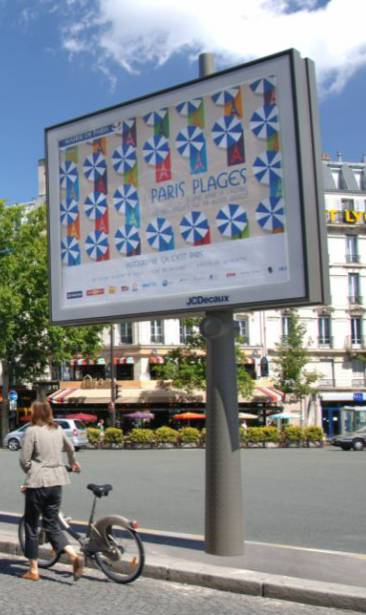
\includegraphics[width=1.61944in,height=2.72917in]{13-MAS-MS/Cours/pandoc/media/image86.jpeg}Le panneau publicitaire déroulant, appartenant à la catégorie des MUPI (Mobilier Urbain Pour l'Information), est un objet installé dans l'espace public. C'est un media de masse qui permet de toucher le consommateur sur son lieu de vie. La société JC DECAUX qui installe des mobiliers urbains fixes s'est intéressée depuis longtemps à pouvoir toucher un maximum de personnes grâce à l'utilisation de ces panneaux.

En effet, on a longtemps utilisé des panneaux fixes mais les études réalisées par JC Decaux Wordlink ont permis d'analyser les effets publicitaires de l'introduction du mouvement dans la communication extérieure.

Cette étude, appelée Sutton démontre qu'un panneau en mouvement augmente le contact visuel avec le panneau de 37\%. Ceci signifie que 90\% du trafic aura au moins un contact visuel avec le site durant son passage. Lorsque le panneau est déroulant, plus de deux-tiers de personnes mémorisent la campagne. C'est pourquoi JC DECAUX a été amené à développer ce type de panneau déroulant. L'expérience de JC DECAUX dans ce domaine date de plus de trente ans puisque le premier brevet concernant ce type de panneau a été déposé en décembre 1977.

Le système étudié est le système de panneau type sénior de 8m² qui équipe de nombreuses villes dont Paris. Ce panneau permet de faire défiler successivement dans un sens puis dans l'autre jusqu'à 7 affiches avec un temps d'exposition constant pour chaque affiche.

Le format des affiches rétro éclairées est d'environ 8m².Les affiches sont de dimensions 3200 x 2300mm (largeur x hauteur) avec une surface visible de 3060 x 2230mm.Le dispositif est constitué de deux rouleaux (longueur 3200mm et ∅ 140mm).Le défilement s'effectue à la vitesse de 1m/s avec une rampe d'accélération et de décélération de chacune 1 seconde. Le cycle de défilement pour 4 affiches est le suivant~:

Le temps d'exposition est programmable à distance via un module GSM (Wacom) relié à un automate programmable (Siemens). Ce temps d'exposition est modifiable suivant les termes du contrat avec l'annonceur.

Les affiches étant changées tous les 15 jours, il faut faciliter leur mise en place. Pour cela, elles sont disposées en bandeau et placées sur le rouleau du haut lors de leur installation. La première est une amorce fixée au rouleau du haut avec un adhésif puis elles sont reliées les unes aux autres par un système de zip. La dernière est une amorce qui est également fixée au rouleau du bas par un adhésif. Cet ensemble constitue un bandeau.

Dans la solution actuelle, l'entraînement se fait par deux moteurs asynchrones identiques commandés par deux variateurs scalaires. L'ensemble est géré par l'automate programmable.

\textbf{Réglage de la vitesse du moteur asynchrone}

Le moteur asynchrone est commandé par un variateur de type U/f constant. La vitesse nominale de défilement d'un affiche est de 1m.s\textsuperscript{-1}. Le moteur utilisé est un motoréducteur réfW10DT56L4.

\ul{Objectif de l'étude~:}

\textbf{Vérifier} le dimensionnement du moteur asynchrone et \textbf{régler} la fréquence du variateur afin de répondre au mieux au cahier des charges.

Dans cette étude, on s'intéressera au fonctionnement à vitesse constante. On notera~:

\begin{itemize}
\item
  Ω~: la vitesse angulaire exprimée en rad/s
\item
  N~: la fréquence de rotation exprimée en tr/min
\end{itemize}

Compte tenu de la tension dans l'affiche, on obtient un couple moteur C\textsubscript{m} = 0,28 Nm à une vitesse angulaire Ω\textsubscript{m}~=~139 rad.s\textsuperscript{-1}.

\textbf{1. Déterminer} la puissance \textbf{P\textsubscript{m}} nécessaire en régime permanent.

Les caractéristiques du moteur lorsqu'il est alimenté sur un réseau 50 Hz sont les suivantes~:

P\textsubscript{N}~: puissance nominale sur l'arbre du moteur 120 W

N\textsubscript{N}~: vitesse nominale en sortie d'arbre 1300 tr.min\textsuperscript{-1}

I\textsubscript{N}~: courant nominal à vitesse nominale 0,8 A

cosϕ~: facteur de puissance 0,68

I\textsubscript{D}/I\textsubscript{N}~: courant au démarrage/courant nominal 2,6

C\textsubscript{N}~: couple nominal 0,88 Nm

C\textsubscript{max}/C\textsubscript{N}~: couple maximal/couple nominal 1,9

\textbf{2.} A partir des caractéristiques du moteur et de la réponse à la question précédente, \textbf{montrer} que le moteur est largement surdimensionné.

\textbf{3. Donner} l'expression de \textbf{g} en fonction de la vitesse angulaire \textbf{Ω\textsubscript{m}} et la vitesse de synchronisme \textbf{Ω\textsubscript{s}}.

\textbf{4. Donner} l'expression de \textbf{Ω\textsubscript{s}} en fonction de \textbf{ω} (pulsation du réseau) et de \textbf{p} (nombre de paires de pôles) puis \textbf{déterminer p}, \textbf{Ω\textsubscript{s}} et \textbf{N\textsubscript{s}} lorsque le moteur est alimenté par un réseau triphasé à une fréquence de 50 Hz.

\textbf{5.} A partir des données du constructeur, \textbf{déduire} la valeur du glissement au point de fonctionnement nominal \textbf{g\textsubscript{N}}.

On rappelle que l'expression du couple électromagnétique pour un moteur asynchrone est~:

\begin{longtable}[]{@{}
  >{\raggedright\arraybackslash}p{(\columnwidth - 2\tabcolsep) * \real{0.4167}}
  >{\raggedright\arraybackslash}p{(\columnwidth - 2\tabcolsep) * \real{0.5694}}@{}}
\toprule\noalign{}
\begin{minipage}[b]{\linewidth}\raggedright
\[C_{m1} =
\frac{2.C_{\max}}{\frac{g_{
0}}{g} + \frac{g}{g_{0}}}\]
\end{minipage} & \begin{minipage}[b]{\linewidth}\raggedright
C\textsubscript{max}~: couple maximal du moteur

g~: glissement

g\textsubscript{0}~: glissement pour le couple C\textsubscript{max}
\end{minipage} \\
\midrule\noalign{}
\endhead
\bottomrule\noalign{}
\endlastfoot
& \\
\end{longtable}

\textbf{6. Calculer} la valeur\textbf{g\textsubscript{0}} à partir de l'expression du couple moteur\textbf{C\textsubscript{m1}}.

\textbf{7. Tracer} l'allure de la caractéristique \textbf{C\textsubscript{m}} en fonction de \textbf{g} (pour 0 \textless{} g \textless{} 1) en indiquant les valeurs numériques de C\textsubscript{N}, g\textsubscript{N}, C\textsubscript{max} et g\textsubscript{0} sur la courbe. \textbf{Préciser} la zone de fonctionnement stable du moteur.

En réalité, le rendement de la transmission n'est pas égal à 1. En conséquence, la valeur du couple électromagnétique en fonctionnement normal est C\textsubscript{maff} = 0,3 Nm.

\textbf{8.} Le système fonctionnant à une valeur de couple C\textsubscript{m1} = C\textsubscript{maff} donc inférieure à C\textsubscript{N}, \textbf{montrer} que l'expression du couple moteur peut se mettre sous la forme\(C_{m1} = 2.\frac{g}{g_{0}}.C_{\max}\) et \textbf{en déduire} la valeur du glissement \textbf{g\textsubscript{aff}} pour le couple \textbf{C\textsubscript{maff}}.

\textbf{9. Montrer} que l'expression du couple peut s'exprimer par C\textsubscript{m1} = λ.(Ω\textsubscript{s} - Ω\textsubscript{m}). \textbf{Préciser} l'expression de λ.

On sait que dans le modèle équivalent du moteur asynchrone on a~:

\begin{longtable}[]{@{}
  >{\raggedright\arraybackslash}p{(\columnwidth - 4\tabcolsep) * \real{0.4861}}
  >{\raggedright\arraybackslash}p{(\columnwidth - 4\tabcolsep) * \real{0.1111}}
  >{\raggedright\arraybackslash}p{(\columnwidth - 4\tabcolsep) * \real{0.3750}}@{}}
\toprule\noalign{}
\begin{minipage}[b]{\linewidth}\raggedright
\[C_{\max} =
\frac{3pV^{2}}{2L_{2}\omega ²}\]
\end{minipage} & \begin{minipage}[b]{\linewidth}\raggedright
et
\end{minipage} & \begin{minipage}[b]{\linewidth}\raggedright
\[g_{0} = \fr
ac{R_{2}}{L_{2}\omega}\]
\end{minipage} \\
\midrule\noalign{}
\endhead
\bottomrule\noalign{}
\endlastfoot
V~: la tension simple aux bornes d'un enroulement

L\textsubscript{2}~: l'inductance secondaire ramenée au primaire

R\textsubscript{2}~: la résistance rotorique secondaire ramenée au primaire & & \\
\end{longtable}

\textbf{10. Justifier} que λ est constant lorsque l'on commande le moteur avec un variateur de vitesse à V/f constant.

Dans la suite du problème, on prendra λ = 0,0453 N.m.s.rad\textsuperscript{-1}.

\textbf{11.} Sachant que le moteur doit tourner à la vitesse Ω\textsubscript{m} = 139 rad.s\textsuperscript{-1} avec un couple C\textsubscript{maff} = 0,3 Nm pour respecter le cahier des charges, quelle devra être la vitesse de synchronisme \textbf{Ω\textsubscript{s}}~? \textbf{En déduire} la valeur de la fréquence f\textsubscript{v} à programmer dans le variateur de vitesse du moteur pour respecter le cahier des charges.

\textbf{\ul{\hfill\break
}}

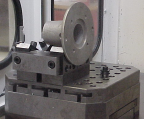
\includegraphics[width=0.65366in,height=0.53947in]{13-MAS-MS/Cours/pandoc/media/image87.png}\textbf{ÉTUDE DE L'ENTRAÎNEMENT DE LA BROCHE D'UN CENTRE D'USINAGE}


\includegraphics[width=1.35556in,height=0.38889in]{13-MAS-MS/Cours/pandoc/media/image77.png} \emph{(\ul{Source~:} Concours CCP TSI 2002)}

\textbf{Mise en situation}

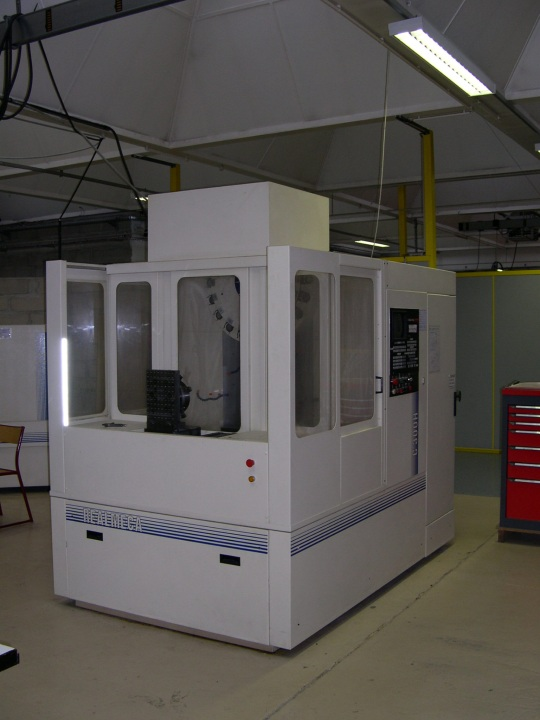
\includegraphics[width=1.95in,height=2.21667in]{13-MAS-MS/Cours/pandoc/media/image88.jpeg}Le système, objet de ce problème, est un centre d\textquotesingle usinage horizontal (cf.~photo) palettisé, à commande numérique quatre axes (X, Y, Z et B).

Ce centre d\textquotesingle usinage, de conception moderne, a été développé afin d\textquotesingle assurer une très haute précision et des performances élevées. Le bâti, en béton de synthèse précontraint, est renforcé de fibres et matériaux spéciaux. Il apporte à cette machine d\textquotesingle excellentes caractéristiques d\textquotesingle amortissement des vibrations.

Les guidages sont assurés par des glissières sur rails prismatiques et cages à aiguilles. Le tout offre un ensemble sans jeu, compact, rigide et graissé à vie.

L\textquotesingle entraînement de la table en X et Z et de la broche en Y est assuré par des moteurs asynchrones triphasés et des systèmes vis / écrou à billes de précision. Le contrôle de position est assuré par des codeurs incrémentaux. Le travail qui suit concerne l\textquotesingle étude de l'alimentation du moteur dela broche.

\begin{quote}
Présentation de la chaîne de conversion de l'énergie
\end{quote}

u\textsubscript{T}(t) = Û\textsubscript{T}.sinωt = U\textsubscript{T}.√2.sinωt soit u\textsubscript{T}(θ) = Û\textsubscript{T}.sinθ = U\textsubscript{T}.√2.sinθ en posant θ = ωt

En sortie du redresseur (redresseur monophasé non commandé), le rôle du filtre est de~:

\begin{quote}
Lisser le courant fourni par le redresseur

Fournir une tension parfaitement continue à l'onduleur de tension
\end{quote}

\textbf{Etude de la charge mécanique}

\ul{Objectif de l'étude~:}

\textbf{Déterminer} les caractéristiques de la machine pour son fonctionnement nominal et les limites de fonctionnement de l'ensemble machine+charge

Le moteur utilisé a les caractéristiques suivantes pour une alimentation à 50 Hz~:

\begin{longtable}[]{@{}
  >{\raggedright\arraybackslash}p{(\columnwidth - 10\tabcolsep) * \real{0.1579}}
  >{\raggedright\arraybackslash}p{(\columnwidth - 10\tabcolsep) * \real{0.1447}}
  >{\raggedright\arraybackslash}p{(\columnwidth - 10\tabcolsep) * \real{0.1711}}
  >{\raggedright\arraybackslash}p{(\columnwidth - 10\tabcolsep) * \real{0.1842}}
  >{\raggedright\arraybackslash}p{(\columnwidth - 10\tabcolsep) * \real{0.1579}}
  >{\raggedright\arraybackslash}p{(\columnwidth - 10\tabcolsep) * \real{0.1579}}@{}}
\toprule\noalign{}
\endhead
\bottomrule\noalign{}
\endlastfoot
P\textsubscript{N} & C\textsubscript{N} & n\textsubscript{N} & I\textsubscript{N} & C\textsubscript{d} & C\textsubscript{max} \\
{[}kW{]} & {[}Nm{]} & {[}tr/min{]} & {[}A{]} & C\textsubscript{N} & {[}Nm{]} \\
\textbf{5,35} & \textbf{35} & \textbf{1460} & \textbf{9,5} & \textbf{2,4} & \textbf{89,3} \\
\end{longtable}

P\textsubscript{N}: puissance nominale C\textsubscript{N} : couple nominal n\textsubscript{N}: vitesse nominale du rotor

I\textsubscript{N}: courant nominal C\textsubscript{d}/C\textsubscript{N}: rapport entre le couple de démarrage et C\textsubscript{N} C\textsubscript{max}: couple maximal

Toutes les pertes de la machine sont négligées, exceptées les pertes Joules rotoriques.

\textbf{7.} A partir des données constructeur dans le cas où la machine est alimentée par le réseau industriel \textbf{230 V / 400 V} et pour une utilisation au point nominal de la machine, \textbf{déterminer} les grandeurs suivantes :

\begin{itemize}
\item
  Le nombre de paires de pôles \textbf{p} de la machine
\item
  La fréquence de rotation \textbf{N\textsubscript{s}}, exprimée en tr/min du champ \textgreater{} statorique
\item
  Le glissement nominal \textbf{g\textsubscript{N}}
\item
  La puissance transmise au rotor \textbf{P\textsubscript{tr}}
\item
  Les pertes Joules rotoriques \textbf{P\textsubscript{jr}}
\item
  Le rendement \textbf{η}du moteur
\item
  Le facteur de puissance \textbf{cos ϕ}
\end{itemize}

Dans le plan couple-vitesse, le lieu de fonctionnement autorisé pour la machine d'entraînement est limité par les caractéristiques suivantes~:

\begin{itemize}
\item
  De 0 à 1500 tr/min~: C\textsubscript{motMAX} = 35 Nm
\item
  De 1500 tr/min~à 6000 tr/min~: P\textsubscript{uMAX} = C\textsubscript{motMAX}Ω = 5,35 kW
\end{itemize}

avec Ω vitesse de rotation mécanique en rad/s.

Entre la machine d'entraînement et la charge mécanique, il y a une boite de vitesse, que l'on considèrera sans pertes, qui comporte deux rapports de réduction. Le couple résistant de la charge mécanique ramené au niveau du moteur d'entraînement peut s'exprimer par~:

\begin{itemize}
\item
  C\textsubscript{res} = C\textsubscript{01}+k\textsubscript{1}Ω pour le premier rapport de réduction (pour 0 ≤ \textgreater{} N ≤ 1000 tr/min)
\item
  C\textsubscript{res} = C\textsubscript{02}+k\textsubscript{2}Ω pour le second rapport de réduction (pour N \textgreater{} \textgreater{} 1000 tr/min)
\end{itemize}

avec C\textsubscript{01} = 12 Nm, k\textsubscript{1} = 0,15 Nm/rad.s\textsuperscript{-1}, C\textsubscript{02} = 1 Nm et k\textsubscript{2} = 0,0125 Nm/rad.s\textsuperscript{-1}.

\textbf{8. Tracer} dans le plan couple-vitesse, \textbf{C(Ω)}, le lieu de fonctionnement autorisé pour le moteur d'entraînement et les caractéristiques de la charge.

\textbf{9.} A partir du graphe précédent, à Ω = 0 rad/s, \textbf{indiquer} la valeur maximale que peut prendre le couple accélérateur (C\textsubscript{acc} = C\textsubscript{mot} - C\textsubscript{res}).

\textbf{10a. Indiquer} le point de fonctionnement atteint avec le premier rapport de réduction.

\textbf{10b.} Lorsque la vitesse atteint 1000 tr/min, on enclenche le second rapport de réduction. \textbf{Donner} alors la valeur du couple accélérateur \textbf{C\textsubscript{acc}} et le point de fonctionnement qui peut être atteint.

\textbf{Etude de la machine asynchrone et de l'onduleur de tension}

\ul{Objectifs de l'étude~:}

\textbf{Déterminer} le couple accélérateur maximal possible avec l'association onduleur+MAS et la commande scalaire de type U/f = cte utilisée.

\textbf{Déterminer} la fréquence d'alimentation permettant d'obtenir le couple accélérateur maximal possible au démarrage

Afin de faire varier la fréquence de rotation de la broche, l'onduleur de tension permet de délivrer à la machine asynchrone des tensions alternatives sinusoïdales de fréquence et d'amplitude variables.

On note \textbf{v\textsubscript{1}(t)}, \textbf{v\textsubscript{2}(t)} et \textbf{v\textsubscript{3}(t)} les tensions simples appliquées aux bornes de chaque phase de la machine asynchrone.

avec~: 
\includegraphics{13-MAS-MS/Cours/pandoc/media/image90.wmf}, \textbf{U\textsubscript{C}} étant la tension constante en entrée de l'onduleur de tension, U\textsubscript{c} = 650V

\textbf{k} est un paramètre de commande~: k ∈ {[}0;1{]}

ω = 2πf où \textbf{f} est la fréquence des tensions en sortie de l'onduleur

On désire maintenir constant le rapport de l'amplitude de la tension sur la fréquence. Pour une fréquence de 50 Hz, la tension efficace entre phases, notée \textbf{U}, atteint la valeur limite de 400 V. La tension simple a une valeur efficace notée V\textsubscript{eff} = 230V. La commande utilisée pour l'onduleur est de type U/f = cte.

\textbf{11. Tracer} la courbe donnant le coefficient \textbf{k} en fonction de la fréquence et ceci pour une fréquence \textbf{f} comprise entre \textbf{0} et \textbf{80 Hz}.

On donne le schéma simplifié équivalent d'une phase de la machine asynchrone ci-contre.

\ul{Application numérique~:}

V\textsubscript{eff} = 230 V~; ω = 2πf rad/s~; p = 2~; L\textsubscript{m} = 180 mH~; L\textsubscript{f} = 18 mH~; R = 0,77 Ω

\textbf{12.} En calculant la puissance électromagnétique dissipée dans la résistance \textbf{R/g}, \textbf{donner} l'expression du couple électromagnétique \textbf{C\textsubscript{em}}.

\textbf{13. Donner} l'expression du couple électromagnétique maximal puis \textbf{calculer} sa valeur numérique pour f = 50 Hz.

Sur le document réponse ont été représentées quatre caractéristiques "couple électromagnétique en fonction de la vitesse de rotation" de la machine asynchrone alimentée par l'onduleur de tension.

\textbf{14.} Pour chaque caractéristique, \textbf{déterminer} graphiquement la vitesse de synchronisme (exprimée en tr/min), le couple maximum et en déduire la fréquence et la valeur efficace des tensions appliquées. Les résultats seront présentés dans un tableau.

\textbf{15.} Sachant que le couple résistant est constant et a une valeur de 35 Nm, \textbf{déterminer} graphiquement pour chaque caractéristique, le point de fonctionnement mécanique (couple et vitesse) et en déduire le point de fonctionnement électrique* (valeurs efficaces des tensions simples et des courants de ligne). On présentera les résultats dans un tableau.

\emph{* On pourra établir l'expression de l'impédance complexe.}

\textbf{16 .}A Ω = 0, \textbf{indiquer} le couple accélérateur maximum que l'on peut obtenir. \textbf{En déduire} la fréquence f d'alimentation.

\textbf{\hfill\break
}

\textbf{DOCUMENT RÉPONSE}

\textbf{\ul{\hfill\break
}}

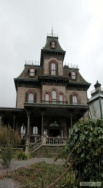
\includegraphics[width=0.46875in,height=0.625in]{13-MAS-MS/Cours/pandoc/media/image91.jpeg}\textbf{MAISON HANTEE}


\includegraphics[width=1.35556in,height=0.38889in]{13-MAS-MS/Cours/pandoc/media/image77.png} \emph{(\ul{Source} : ATS 2009)}

\textbf{Mise en situation}

Vieilles pierres, couloirs sans fin et pièges maléfiques ... il faut avoir le cœur bien accroché pour s\textquotesingle aventurer dans ces lieux ... Cette installation est composée de seize véhicules indépendants roulant sur une piste béton de 192 mètres. Cette piste reçoit en son centre un rail de guidage qui fixe la trajectoire des véhicules.

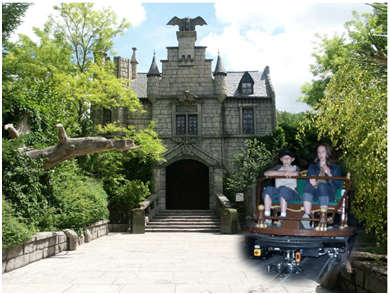
\includegraphics[width=2.84931in,height=2.26181in]{13-MAS-MS/Cours/pandoc/media/image92.png}Chaque voiture peut recevoir deux personnes au maximum. Les passagers ne conduisent pas, ils sont uniquement spectateurs. Ils sont assis sur une nacelle tournante, libre en rotation. Un système de contrepoids placé sous l\textquotesingle assise, ainsi que l\textquotesingle inclinaison de la piste, permettent une bonne orientation des visiteurs devant les scènes du décor.

Une voie de garage peut contenir sept véhicules permettant ainsi le délestage de la piste pour adapter le nombre de véhicules à la fréquentation.

Un opérateur proche du quai d\textquotesingle embarquement a en charge l\textquotesingle exploitation, il doit gérer les flux des départs, contrôler les débarquements et surveiller l\textquotesingle évolution sur la piste.

\textbf{\ul{Données~:}}

\begin{itemize}
\item
  Vitesse du véhicule~: V\textsubscript{C} = 1 à 1,3 m/s = V\textsubscript{M}
\item
  Variation de vitesse maximale tolérée~: 10\%
\item
  Pente maximale en montée~: 6\%~; en descente~: 7\%
\item
  Tension d'alimentation~: U\textsubscript{1}, réseau EDF (250 V, 50 Hz)
\end{itemize}

L\textquotesingle analyse de l\textquotesingle activité du service maintenance fait ressortir les points suivants~:

\begin{itemize}
\item
  Changements fréquents des pare-chocs dus aux collisions entre véhicules
\item
  Remplacement des moteurs (6 moteurs par saison)

  \textbf{Étude de l'alimentation de la MAS}
\end{itemize}

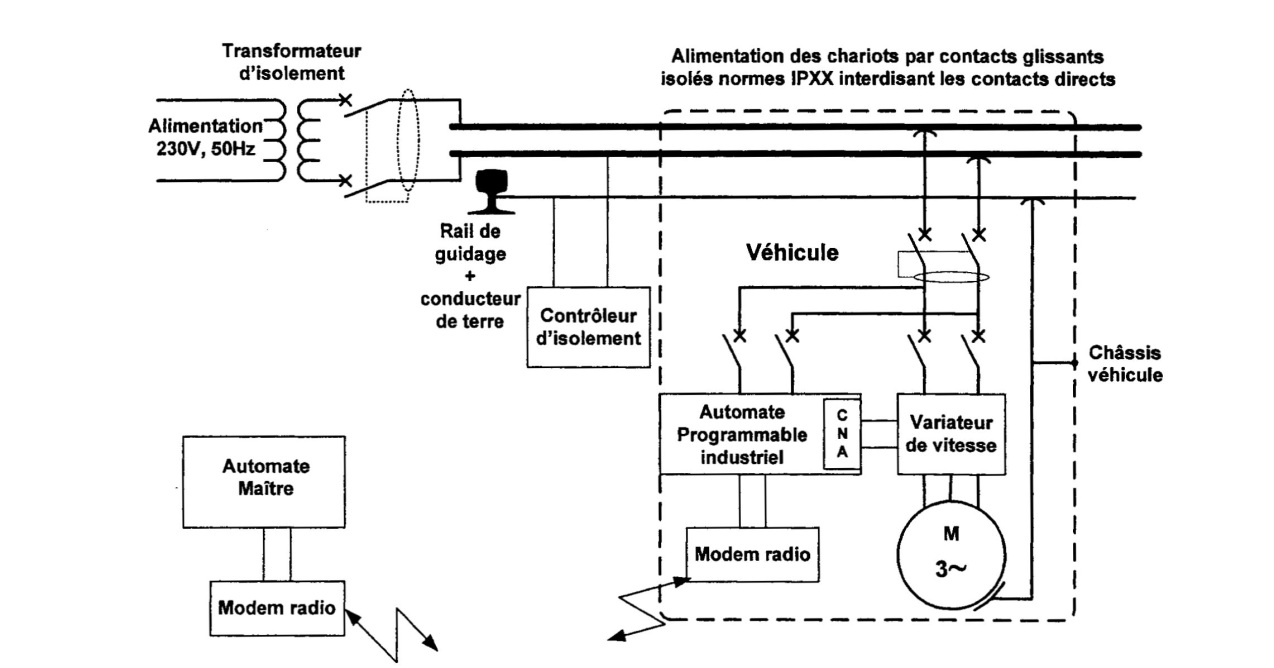
\includegraphics[width=4.66389in,height=2.86736in]{13-MAS-MS/Cours/pandoc/media/image93.jpeg}La solution initiale utilisant une machine à courant continu pour chaque véhicule n\textquotesingle a pas été retenue par le service maintenance qui a préféré la remplacer par un moteur asynchrone triphasé associé à un variateur de vitesse (convertisseur de fréquence). La raison essentielle de ce choix est la maintenance réduite de ce type de moteur par rapport au moteur à courant continu (pas d\textquotesingle usure de balais, pas de court-circuit dû à la présence de poussière de carbone dans les moteurs).

Schéma de principe de l\textquotesingle installation

L\textquotesingle alimentation des véhicules se fait en 230 V, 50 Hz, chaque véhicule est équipé d\textquotesingle un automate programmable industriel, tous les automates sont en liaison avec un automate maître fixe situé dans la station par un réseau modbus.

Les moteurs asynchrones triphasés SEW modèle DV 100 M4 sont alimentés par des variateurs de vitesse, l\textquotesingle entrée de consigne de ces variateurs est fournie par une sortie analogique de l\textquotesingle automate. La transmission mécanique est dimensionnée de manière à ce que la vitesse de translation du chariot soit de 1,3 m/s lorsque le moteur tourne à n~=~1400 tr/min, le couple utile à la sortie du moteur est compris entre \textbf{10 Nm} et \textbf{-4 Nm}.

L\textquotesingle expression du couple électromagnétique du moteur asynchrone en fonction du glissement déduite des propriétés du schéma équivalent monophasé est de la forme~: \(C_{em} = \frac{3U^{2}}{\Omega_{S}}.\frac{R_{2}.g}{R_{2}^{2} + X_{2}^{2}.g^{2}}\)

Avec~: C\textsubscript{em}~: couple électromagnétique

\begin{quote}
U~: valeur efficace de la tension composée

Ω\textsubscript{S}~: vitesse angulaire de rotation du champ tournant

R\textsubscript{2}~: résistance d\textquotesingle une phase du rotor, ramenée au stator

X\textsubscript{2}~: réactance d\textquotesingle une phase du rotor ramenée au stator avec X\textsubscript{2} = L\textsubscript{2}ω~; ω = 2πf où f est la fréquence des courants statoriques

\(g = \frac{\Omega_{S} - \omega_{m}}{\Omega_{S}}\)~: glissement

ω\textsubscript{m}~: vitesse angulaire de rotation du rotor du moteur
\end{quote}

Le moteur est connecté en triangle.

Le couple de pertes est négligé~: C\textsubscript{em} = C\textsubscript{u} (couple utile).

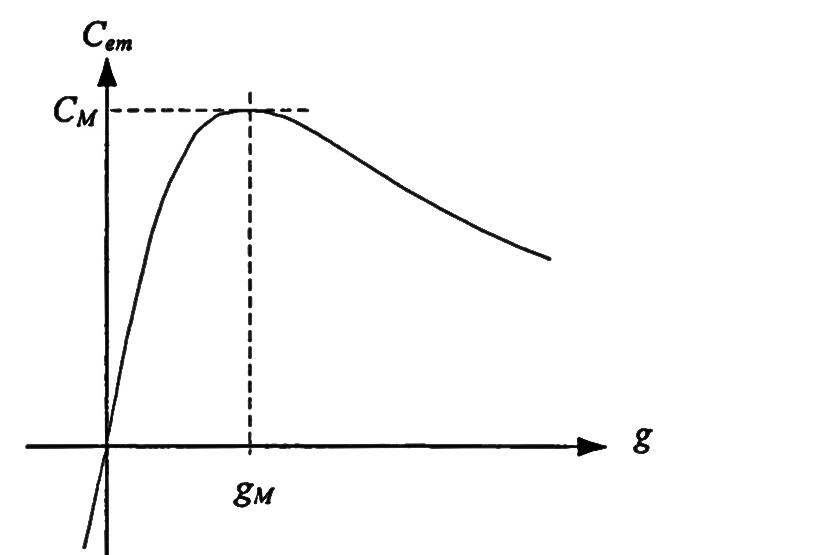
\includegraphics[width=3.01875in,height=2.44167in]{13-MAS-MS/Cours/pandoc/media/image94.jpeg}Dans la zone de fonctionnement du moteur, la caractéristique C\textsubscript{em}~=~f(g) peut être modélisée par une droite paramétrée par Ω\textsubscript{S}. Il convient de déterminer l\textquotesingle équation de cette droite.

Figure 1: Caractéristique C\textsubscript{em}=f(g)

La caractéristique C\textsubscript{em} = f(g) passe par un maximum C\textsubscript{M} pour une valeur g\textsubscript{M} du glissement (voir figure ci-contre).

\textbf{1.} En utilisant les propriétés de la dérivée, \textbf{déterminer} l\textquotesingle expression de g\textsubscript{M} en fonction de R\textsubscript{2} et X\textsubscript{2}.

\textbf{2. Donner} l\textquotesingle expression de C\textsubscript{M} en fonction de U, Ω\textsubscript{S} et X\textsubscript{2}.

\textbf{3. Montrer} que C\textsubscript{em} peut se mettre sous la forme~:

\begin{quote}
\[C_{em} = 2.C_{M}.\frac{x}{1 + x^{2}}\ avec\ x = \frac{g}{g_{M}}\]
\end{quote}

Le moteur utilisé a les caractéristiques suivantes pour une alimentation à 50 Hz :

\begin{longtable}[]{@{}
  >{\raggedright\arraybackslash}p{(\columnwidth - 16\tabcolsep) * \real{0.1486}}
  >{\raggedright\arraybackslash}p{(\columnwidth - 16\tabcolsep) * \real{0.0946}}
  >{\raggedright\arraybackslash}p{(\columnwidth - 16\tabcolsep) * \real{0.0946}}
  >{\raggedright\arraybackslash}p{(\columnwidth - 16\tabcolsep) * \real{0.0946}}
  >{\raggedright\arraybackslash}p{(\columnwidth - 16\tabcolsep) * \real{0.0946}}
  >{\raggedright\arraybackslash}p{(\columnwidth - 16\tabcolsep) * \real{0.0946}}
  >{\raggedright\arraybackslash}p{(\columnwidth - 16\tabcolsep) * \real{0.0946}}
  >{\raggedright\arraybackslash}p{(\columnwidth - 16\tabcolsep) * \real{0.0946}}
  >{\raggedright\arraybackslash}p{(\columnwidth - 16\tabcolsep) * \real{0.0946}}@{}}
\toprule\noalign{}
\endhead
\bottomrule\noalign{}
\endlastfoot
Type moteur

380-415 V & P\textsubscript{N}

(kW) & M\textsubscript{N}

(Nm) & n\textsubscript{N}

(tr/ min) & \begin{minipage}[t]{\linewidth}\raggedright
I\textsubscript{N}

\hfill\break
(A)\strut
\end{minipage} & cosϕ & l \textsubscript{A}/ l\textsubscript{N} & J\textasciitilde{} Mot\textasciitilde{}

( kg.m \textsuperscript{2}) & M\textasciitilde{} max\textasciitilde{}

(Nm) \\
DV 100 M4 & 2,2 & 15 & 1410 & 4,9 & 0,83 & 5,9 & 53 & 40 \\
\end{longtable}

\begin{quote}
P\textsubscript{N}: puissance nominale cosϕ : facteur de puissance

M\textsubscript{N} : couple nominal l\textsubscript{A}/l\textsubscript{N} : rapport entre le courant de démarrage et I\textsubscript{N}

n\textsubscript{N}: vitesse nominale du rotor J\textsubscript{mot} : inertie du moteur

I\textsubscript{N}: courant nominal M\textsubscript{max} : couple maximal
\end{quote}

\textbf{4. Exprimer} la vitesse angulaire de rotation du champ tournant Ω\textsubscript{S} en fonction de la fréquence f des courants statoriques et du nombre de paires de pôles p.

\textbf{5.} En utilisant les caractéristiques du moteur et en considérant qu\textquotesingle en fonctionnement nominal le glissement est faible, \textbf{déterminer} le nombre de paires de pôles p du moteur asynchrone.

\textbf{6.} En utilisant le résultat de la question \textbf{3} et les caractéristiques du moteur, \textbf{calculer} la valeur de g\textsubscript{M} sachant que x est inférieur à 1.

Les résultats précédents permettent d\textquotesingle obtenir une expression linéarisée de la caractéristique de couple C\textsubscript{em} = f(g) autour de la vitesse de synchronisme. L\textquotesingle expression de C\textsubscript{em} devient alors C\textsubscript{em} = 1,65×Ω\textsubscript{s}×g.

Nous allons déterminer la fréquence de la tension d\textquotesingle alimentation pour que le chariot se déplace à 1,3 m/s, lorsque le couple moteur est de 10 Nm.

\textbf{7. Donner} l\textquotesingle expression de C\textsubscript{em} en fonction de f, p et ω\textsubscript{m} (vitesse angulaire de rotation du rotor en rad/s).

\textbf{8. Calculer} la fréquence f des courants d\textquotesingle alimentation du moteur pour que le chariot se déplace à 1,3 m/s lorsque le couple moteur est de 10 Nm.

Le couple pouvant devenir négatif, la structure du convertisseur doit permettre cette inversion. Il faut d\textquotesingle abord s\textquotesingle assurer de la réversibilité du système utilisé.

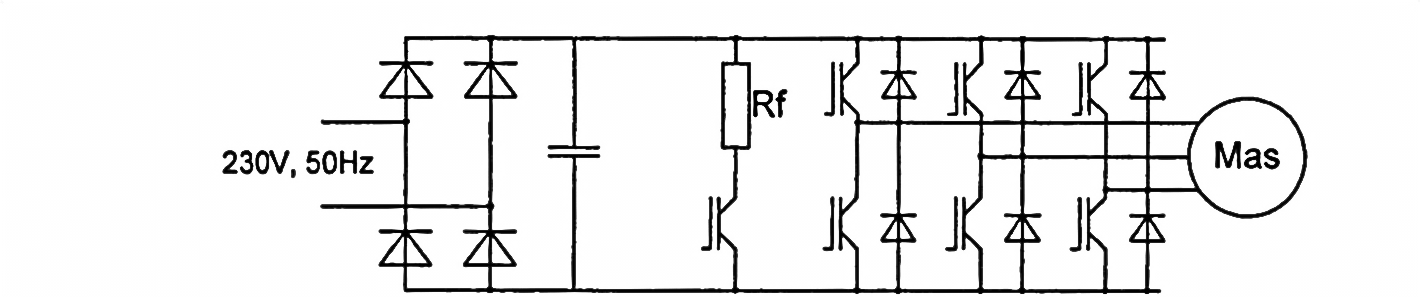
\includegraphics[width=5in,height=1.21698in]{13-MAS-MS/Cours/pandoc/media/image95.png}

Schéma de principe du convertisseur de fréquence

Les transistors sont considérés comme des interrupteurs commandés et le dispositif de commande n\textquotesingle est pas représenté.

\textbf{9.} Le schéma de principe du convertisseur de fréquence est représenté sur la figure ci-dessus. \textbf{Conclure} en explicitant la réponse sur la réversibilité demandée.

Le cahier des charges impose une variation de vitesse maximale tolérée de 10\%. Nous allons vérifier ce critère d\textquotesingle appréciation sur cette nouvelle solution.

\textbf{10.} La fréquence des courants d\textquotesingle alimentation étant celle calculée à la question \textbf{8}, \textbf{calculer} la vitesse de rotation du moteur lorsque le couple passe à -4 Nm.

\textbf{11.} En considérant les variations extrêmes de la vitesse en fonction des variations du couple, \textbf{conclure} quant à la nécessité de réguler la vitesse.

\textbf{12. Conclure} quant aux avantages et aux inconvénients de l\textquotesingle utilisation des moteurs asynchrones.

\textbf{\ul{\hfill\break
}}


\includegraphics[width=1.35556in,height=0.38889in]{13-MAS-MS/Cours/pandoc/media/image77.png}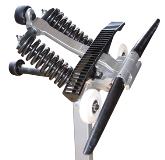
\includegraphics[width=0.7503in,height=0.72642in]{13-MAS-MS/Cours/pandoc/media/image96.png}

\textbf{TELESIEGE DEBRAYABLE 6 PLACES}

\emph{(\ul{Source :} CCP TSI 2016)}

\textbf{Mise en situation}

L'étude proposée dans cet exercice porte sur les moteurs de secours du télésiège débrayable 6 places (TSD6) «~Biollay~», mis en activité récemment au sein de la station de Courchevel. Il a été conçu par la société Poma.

\begin{figure}
\centering
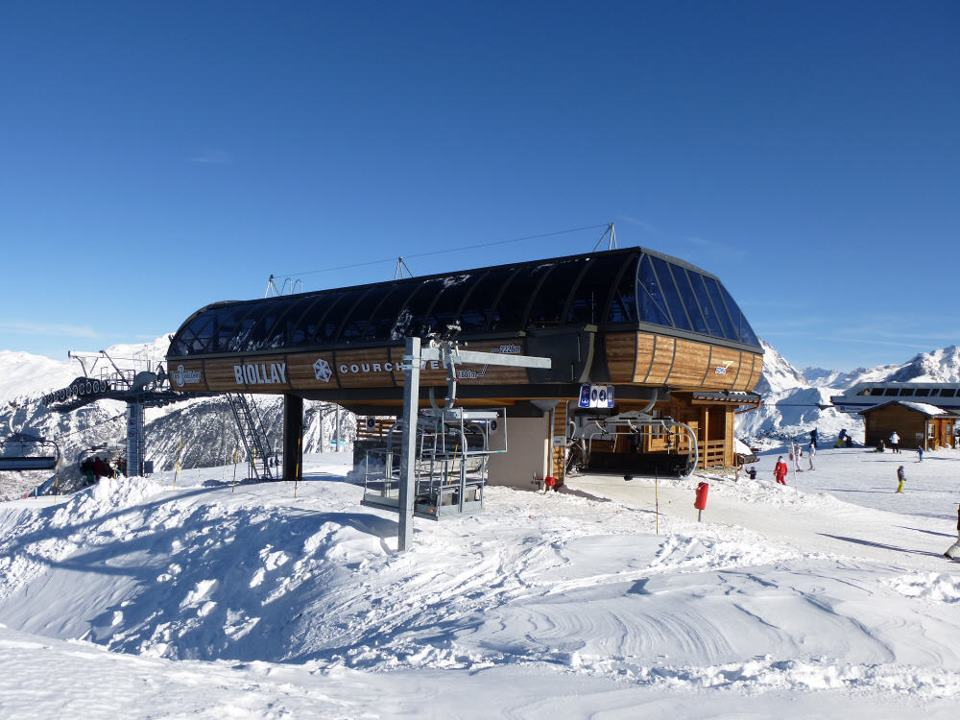
\includegraphics[width=5.13194in,height=2.38333in]{13-MAS-MS/Cours/pandoc/media/image97.jpeg}
\caption{C:\textbackslash Users\textbackslash Benoit\textbackslash Documents\textbackslash CPGE\textbackslash Concours\_TSI\textbackslash Sujets\_écrit\textbackslash Sujet\_écrit\_2015\textbackslash Ressources\textbackslash538055\_469097636460151\_1077262434\_n.jpg}
\end{figure}

\ul{Extrait du cahier des charges~:}

\begin{longtable}[]{@{}
  >{\raggedright\arraybackslash}p{(\columnwidth - 2\tabcolsep) * \real{0.6486}}
  >{\raggedright\arraybackslash}p{(\columnwidth - 2\tabcolsep) * \real{0.3243}}@{}}
\toprule\noalign{}
\begin{minipage}[b]{\linewidth}\raggedright
Vitesse du câble en marche secours
\end{minipage} & \begin{minipage}[b]{\linewidth}\raggedright
de 0,8 m.s\textsuperscript{-1} à 1,8 m.s\textsuperscript{-1}
\end{minipage} \\
\midrule\noalign{}
\endhead
\bottomrule\noalign{}
\endlastfoot
Nombre de moteurs en marche secours normal & 2 \\
Nombre de moteurs en marche secours dégradé & 1 \\
\end{longtable}

\ul{Grandeurs et valeurs numériques~:}

\begin{longtable}[]{@{}
  >{\raggedright\arraybackslash}p{(\columnwidth - 2\tabcolsep) * \real{0.3108}}
  >{\raggedright\arraybackslash}p{(\columnwidth - 2\tabcolsep) * \real{0.6622}}@{}}
\toprule\noalign{}
\begin{minipage}[b]{\linewidth}\raggedright
\textbf{Eléments}
\end{minipage} & \begin{minipage}[b]{\linewidth}\raggedright
\textbf{Caractéristiques et notations}
\end{minipage} \\
\midrule\noalign{}
\endhead
\bottomrule\noalign{}
\endlastfoot
2 Moteurs de secours asynchrones triphasés SIEMENS 75 kW de référence 1LE1501-2DA03-4AA4 & Couple d'un seul moteur de secours~: C\textsubscript{ms} \\
& Vitesse de rotation~: ω\textsubscript{ms} \\
& Puissance utile~: P\textsubscript{u} = 75 kW \\
& Tension nominale~: U = 400 V \\
& Courant nominal~: I = 133 A \\
& Fréquence~: f = 50 Hz \\
& Vitesse de rotation nominale~: N\textsubscript{n} = 2 978 tours/min \\
& Rendement~: η = 93,8 \% \\
& Facteur de puissance~: cosϕ = 0,87 \\
2 Réducteurs par moteur de secours & Rapport de réduction primaire~: r\textsubscript{1} = ω\textsubscript{ms}/ω\textsubscript{pignon} = 32,7 \\
& Réduction secondaire~: r\textsubscript{2}~; couronne~: Z\textsubscript{c}\(\ \)= 220 et pignon~: Z\textsubscript{p}\(\ \)= 16 \\
& Rendement~des deux réducteurs~: η = 1 \\
Poulie motrice & Rayon~: R\textsubscript{p} = 2,45 m \\
\end{longtable}

\textbf{Couple moteur nécessaire}

\ul{Objectif~:} \textbf{Déterminer} le couple des moteurs de secours nécessaire à l'évacuation des skieurs.

Lors d'un dysfonctionnement de la motorisation principale ou lors d'une coupure électrique, les deux moteurs électriques de secours prennent le relais et permettent d'évacuer les skieurs. Il est alors nécessaire de désaccoupler le réducteur principal de la poulie motrice. En cas de secours, deux moteurs électriques asynchrones sont donc utilisés. La puissance de chaque moteur est transmise à un premier réducteur de rapport de réduction r\textsubscript{1}, puis transmise à un ensemble pignon-couronne, la couronne étant solidaire de la poulie motrice. Ceci est illustré sur la figure ci-contre. Le nombre de dents de la couronne est noté Z\textsubscript{c} et le nombre de dents du pignon est noté Z\textsubscript{p}.

\ul{Hypothèses}

On considérera les cas limites de fonctionnement~:

\begin{itemize}
\item
  Au début de l'évacuation à la montée, 100 \% des sièges sont pleins, \textgreater{} entrainant une tension du câble T\textsubscript{B}~=~337~000 N
\item
  A la fin de l'évacuation à la montée, 100 \% des sièges sont vides \textgreater{} entrainant une tension du câble T\textsubscript{B}~=~282~000~N
\end{itemize}

Du début à la fin de l'évacuation, les sièges à la descente sont vides entrainant une tension du câble T\textsubscript{A}~=~260~000~N

On considérera que l'on se place en régime établi et que les liaisons sont parfaites.

\textbf{1. Donner} l'expression de C\textsubscript{ms} en fonction de T\textsubscript{B}, T\textsubscript{A} et des différentes caractéristiques introduites dans la Mise en situation. \textbf{Faire} l'application numérique de C\textsubscript{ms} au début de l'évacuation et à la fin de l'évacuation.

Pour la suite, on prendra les valeurs suivantes~:

\begin{itemize}
\item
  C\textsubscript{ms}\(\ \)= 210 N.m au début de l'évacuation
\item
  C\textsubscript{ms}\(\ \)= 60 N.m à la fin de l'évacuation

  \textbf{Validation des moteurs de secours}
\end{itemize}

\ul{Objectif~:} \textbf{Valider} la solution retenue. Les moteurs doivent assurer la marche de secours avec une vitesse du câble comprise entre 0,8 m.s\textsuperscript{-1} et 1,8 m.s\textsuperscript{-1} en marche avant ou arrière. Dans le cas d'une défaillance d'un des moteurs de secours, l'autre pourra assurer le fonctionnement.

La solution choisie par la société Poma est le moteur asynchrone triphasé SIEMENS 75 kW de référence 1LE1501-2DA03-4AA4. Les caractéristiques données par le constructeur sont regroupées dans la Mise en situation.

\textbf{2.} Pour une utilisation au point de fonctionnement nominal de la machine, \textbf{déterminer} les grandeurs suivantes~:

\begin{itemize}
\item
  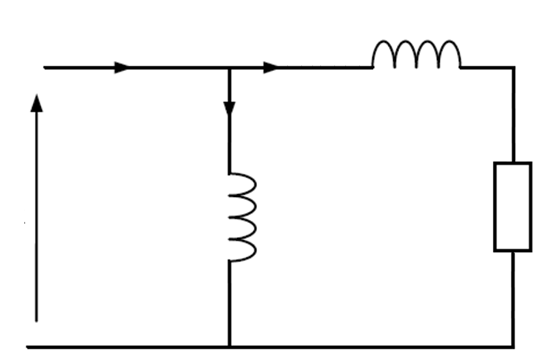
\includegraphics{13-MAS-MS/Cours/pandoc/media/image98.png}\{width=``2.986111111111111in'' \textgreater{} height=``1.8541666666666667in''\}La fréquence de rotation N\textsubscript{S}, \textgreater{} exprimée en tours par minute du champ tournant statorique
\item
  Le nombre de paires de pôles p de la machine
\item
  Le glissement nominal g\textsubscript{n}.
\end{itemize}

Le choix d'un moteur ne peut être validé que si celui-ci peut assurer le fonctionnement dans le cas d'un mode dégradé (un seul moteur fonctionnant).

Pour cela, des essais à vide et à rotor bloqué, donnés par le constructeur, ont permis d'établir le modèle équivalent d'une phase du moteur asynchrone.

\begin{quote}
V\textsubscript{1} = 230 V R'\textsubscript{2} = 10,5 mΩ X'\textsubscript{2} = 0,23 Ω X\textsubscript{0} = 4,76 Ω
\end{quote}

Modèle équivalent d'une phase du moteur asynchrone

\textbf{3. Déterminer} l'expression de la valeur efficace du courant I'\textsubscript{2} en fonction de V\textsubscript{1}, X'\textsubscript{2}, R'\textsubscript{2} et g.

Pour la suite, on négligera les pertes mécaniques du rotor, donc le couple mécanique utile sera égal au couple électromagnétique.

\textbf{4a. Déterminer} les expressions de la puissance transmise au rotor P\textsubscript{tr} et de la puissance mécanique P\textsubscript{méca} en fonction de V\textsubscript{1}, X'\textsubscript{2}, R'\textsubscript{2} et g.

\textbf{4b.} \textbf{Montrer} que le couple électromagnétique développé par la machine peut se mettre sous la forme~:

\(C_{ms} = \frac{3.p.V_{1}^{2}}{\omega}.\frac{\frac{R_{2}^{'}}{g}}{\left( \frac{R_{2}^{'}}{g} \right)^{2} + \left( X_{2}^{'} \right)^{2}}\) avec ω = 2.π.f

\textbf{4c. Déterminer} le glissement g\textsubscript{M}\(\ \) tel que le couple électromagnétique C\textsubscript{ms} soit maximal en fonction de R'\textsubscript{2} et de X'\textsubscript{2}. Faire l'application numérique.

Pour la suite, on prendra g\textsubscript{M} = 0,046.

\ul{Fonctionnement «~dégradé~» de la marche de secours}

Remarque~: Les glissements aux points de fonctionnement stables sont \ul{inférieurs} au glissement g\textsubscript{M}.

\textbf{5a.} \textbf{Déterminer} les glissements g'\textsubscript{1} \(\ \)et g'\textsubscript{2} pour des couples moteurs respectifs C'\textsubscript{ms1}~=~420~Nm (début d'évacuation) et C'\textsubscript{ms2}~=~120~N.m (fin d'évacuation).

\textbf{5b. En déduire} les vitesses de translation en début et en fin d'évacuation.

\ul{Conclusion}

\textbf{6.} À partir des résultats obtenus aux questions précédentes, \textbf{valider} le choix du moteur de secours retenu.

\textbf{\ul{\hfill\break
}}

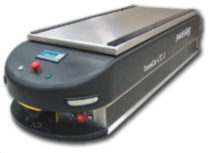
\includegraphics[width=0.99704in,height=0.72642in]{13-MAS-MS/Cours/pandoc/media/image99.png}


\includegraphics[width=1.35556in,height=0.38889in]{13-MAS-MS/Cours/pandoc/media/image77.png}\textbf{VEHICULE AUTO GUIDÉ}

\emph{(\ul{Source :} ATS 2014)}

\textbf{Mise en situation}

Le VAG est un véhicule autonome à guidage laser. Il est utilisé en milieu hospitalier pour le transport de déchets, plateaux repas, linges dans les parties non accessibles au public. Seules des personnes autorisées peuvent y pénétrer. On peut donc considérer qu'il s'agit de zones propres.

L'étude proposée porte sur le respect des conditions de sécurité pour la circulation des chariots à proximité du personnel de l'hôpital.

L'avancement du VAG est assuré par un moteur-roue \textbf{1}. L'arbre \textbf{7} est l'arbre moteur (le moteur n'est pas représenté). L'énergie mécanique est transmise à la roue \textbf{1} par l'intermédiaire d'un train d'engrenages.

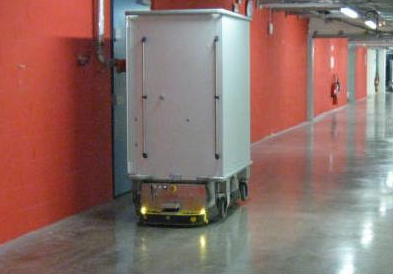
\includegraphics{13-MAS-MS/Cours/pandoc/media/image100.png}

Dans le mouvement de translation rectiligne du chariot, le point A lié au carter \textbf{5}, a pour vitesse 
\includegraphics{13-MAS-MS/Cours/pandoc/media/image101.wmf}. Le roulement de la roue sur le sol \textbf{0} se fait sans glissement.

Avec r rayon de la roue d'entraînement, r\textsubscript{1} le rapport de réduction entre le moteur et la roue, ω\textsubscript{7/6} la vitesse de rotation du rotor en rd·s\textsuperscript{-1}, la vitesse du chariot a pour expression~:

\begin{quote}

\includegraphics{13-MAS-MS/Cours/pandoc/media/image102.wmf} avec r = 105 mm et 
\includegraphics{13-MAS-MS/Cours/pandoc/media/image103.wmf}
\end{quote}

La plage de vitesse stabilisée en ligne droite du VAG, V\textsubscript{A,5/0}, doit être ajustable entre 0,1 et 1,2 m·s\textsuperscript{-1}.

\ul{Données utiles~:}

La tension continue issue du pack de batterie est de 24 V.

Le moteur est piloté par un variateur de vitesse non étudié ici.

Le moteur est de type asynchrone triphasé couplé par construction en étoile et de caractéristiques nominales suivantes (lecture de la plaque signalétique)~:

\begin{longtable}[]{@{}
  >{\raggedright\arraybackslash}p{(\columnwidth - 2\tabcolsep) * \real{0.5541}}
  >{\raggedright\arraybackslash}p{(\columnwidth - 2\tabcolsep) * \real{0.4189}}@{}}
\toprule\noalign{}
\begin{minipage}[b]{\linewidth}\raggedright
Fréquence nominale d'alimentation du stator f\textsubscript{s} = 110 Hz
\end{minipage} & \begin{minipage}[b]{\linewidth}\raggedright
Tension efficace entre phases U\textsubscript{n} = 14,5 V
\end{minipage} \\
\midrule\noalign{}
\endhead
\bottomrule\noalign{}
\endlastfoot
Vitesse nominale en charge N\textsubscript{n} = 3100 tr·min\textsuperscript{-1} & Puissance utile mécanique P\textsubscript{u} = 850 W \\
Facteur de puissance à charge nominale F\textsubscript{p} = cosφ = 0,79 & Rendement nominal η\textsubscript{n} = 0,76 \\
\end{longtable}

\ul{Remarques~:}

Pour l'étude réalisée (déplacement en ligne droite), le système d'orientation est immobile

On posera N = ω\textsubscript{7/6} × \(\frac{30}{\pi}\)

\textbf{Détermination de la loi entrée sortie entre le variateur et la roue}

A partir des indications et caractéristiques du moteur

\textbf{1. Donner} la relation liant la vitesse de synchronisme N\textsubscript{s} en tr·min\textsuperscript{-1} et la fréquence f en Hz de l'alimentation. On notera p le nombre de paires de pôles.

\textbf{2. Introduire} le glissement g et \textbf{exprimer} la relation liant N\textsubscript{s} et la vitesse du rotor N\textbf{.} \textbf{En déduire} en justifiant par une hypothèse simplificatrice, le nombre de paires de pôles p du moteur et la vitesse de synchronisme N\textsubscript{s}.

\textbf{3. Exprimer} puis \textbf{calculer} le glissement nominal du moteur g\textsubscript{n} en \% et son couple nominal C\textsubscript{n} en Nm.

\textbf{4. Etablir} la relation entre la vitesse du rotor du moteur ω\textsubscript{7/6} en rd·s\textsuperscript{-1}, la fréquence f des tensions de sortie du variateur et le glissement g. \textbf{Déduire} alors la relation entre la vitesse du chariot V\textsubscript{A,5/0}, la fréquence f et le glissement g.

\textbf{5.} En admettant pour le moteur en charge un glissement constant g = 6\%, \textbf{exprimer} la vitesse du chariot sous la forme V\textsubscript{A,5/0} = K·f et \textbf{déterminer} l'expression de K et sa valeur numérique. \textbf{Déduire} la plage de fréquence f nécessaire pour que la vitesse V\textsubscript{A,5/0} du VAG respecte la plage de vitesse fixée plus haut.

La vitesse maximale du moteur est fixée à +2620 tr·min\textsuperscript{-1}.

\textbf{6. Utiliser} l'annexe variateur «~Entrée numérique de contrôle de la vitesse~» et \textbf{donner} en justifiant, la valeur numérique décimale à programmer pour obtenir cette vitesse, puis sous forme binaire les deux octets Byte 0 et Byte 1.

Le couple d'un moteur asynchrone est admis constant si le rapport U/f est également constant. On utilisera le rapport U/f du point nominal.

\textbf{7. Déduire} numériquement la plage de la tension efficace U entre phases nécessaire pour maintenir le couple du moteur constant pour la plage de vitesse considérée. \textbf{Vérifier} sa compatibilité avec la source de tension continue disponible.

\textbf{ANNEXE~: Variateur de roue}

\begin{longtable}[]{@{}
  >{\raggedright\arraybackslash}p{(\columnwidth - 2\tabcolsep) * \real{0.5000}}
  >{\raggedright\arraybackslash}p{(\columnwidth - 2\tabcolsep) * \real{0.4861}}@{}}
\toprule\noalign{}
\begin{minipage}[b]{\linewidth}\raggedright
\textbf{Variateur~: caractéristiques de puissance}
\end{minipage} & \begin{minipage}[b]{\linewidth}\raggedright
\end{minipage} \\
\midrule\noalign{}
\endhead
\bottomrule\noalign{}
\endlastfoot
\includegraphics[width=6.56181in,height=1.90625in]{13-M AS-MS/Cours/pandoc/media/image104 .png} & \\
Housing~: \emph{Boitier}

Nominal battery voltage~: \emph{Tension nominale de la batterie}

Input voltage range permanent~: \emph{Plage de tension d'entrée permanente}

Short time : \emph{Temps court \textless{} 30s} & Nominal output current~: \emph{Courant de sortie nominal}

Maximum output current~: \emph{Courant de sortie maximal}

Output voltage~: \emph{Tension de sortie} \\
\textbf{Variateur~: Paramètres des rampes d'accélération et de décélération} & \\
\includegraphics[width=6.31181in,height=1.63542in]{13-M AS-MS/Cours/pandoc/media/image105 .png} & \\
Par.no.~: \emph{Numéro du paramètre à programmer}

Name~: \emph{Nom du paramètre}

Range~: \emph{Plage de réglage}

Units~: \emph{Unités}

Default~: \emph{Valeur programmée par défaut}

Acceleration ramp~: \emph{Rampe d'accélération}

Deceleration ramp~: \emph{Rampe de décélération}

Rpm/s~: \emph{en tour par minute / seconde (pour l'accélération et la décélération)} & The parameter sets the ramp slope for speed acceleration (increasing numéric rpm) :

\emph{Le paramètre définit la pente de la rampe d\textquotesingle accélération de vitesse (augmentation numérique de la vitesse en tr.min\textsuperscript{-1} pour une seconde)}

The parameter sets the ramp slope for speed deceleration (decreasing numéric rpm) :

\emph{Le paramètre définit la pente de la rampe de décélération de vitesse (diminution numérique de la vitesse en tr.min\textsuperscript{-1} pour une seconde)} \\
\textbf{Variateur~: Entrée numérique de contrôle de la vitesse} & \\
\includegraphics[width=7.00972in,height=0.875in]{13-M AS-MS/Cours/pandoc/media/image106 .png} & \\
Byte~: \emph{Octet}

Low~: \emph{Partie basse}

High~: \emph{Partie haute}

Data~: \emph{Donnée}

Set speed command~: \emph{Définit la commande en vitesse}

\ul{La vitesse est donc définie par un mot de 16 bits incluant le bit de signe à gauche} & Scale~: \emph{Echelle}

L'incrément de vitesse vaut 0,25 ou 1/4 tour.min\textsuperscript{-1}

Range / Setting~:

\emph{Plage numérique programmable / Variation de vitesse correspondante en tr.min\textsuperscript{-1}}

\ul{Le point est pour la plage le séparateur des milliers} \\
\end{longtable}

\textbf{\ul{\hfill\break
}}

\textbf{DEPOSE BAGAGE AUTOMATIQUE}


\includegraphics[width=1.35556in,height=0.38889in]{13-MAS-MS/Cours/pandoc/media/image77.png} \emph{(\ul{Source} : Centrale-Supélec TSI 2018)}

\textbf{Mise en situation}


\includegraphics[width=2.86736in,height=1.80972in]{13-MAS-MS/Cours/pandoc/media/image107.emf}
\includegraphics[width=2.84861in,height=2.00278in]{13-MAS-MS/Cours/pandoc/media/image108.emf}\ul{Présentation du système}

Depuis déjà plusieurs années, le processus d'enregistrement des passagers dans les aéroports est en train de vivre une mutation en évoluant de la « banque d'enregistrement » classique vers une idée de « dépose bagages » automatisée.

Le système de DBA permet au passager de déposer un bagage en toute autonomie.

\ul{Problématique}

La chaine d'énergie du basculeur est notamment constituée d'une machine asynchrone (MAS) triphasée alimentée par un variateur de vitesse connecté au réseau triphasé 230 V / 400 V. La machine asynchrone entraine l'ensemble bielle-manivelle du basculeur via un réducteur de rapport de réduction k = \(\frac{1}{107,7}\)

Compte tenu du glissement dépendant du couple résistant imposé par la charge, la vitesse de rotation de l'arbre de la machine asynchrone en régime établi est différente de sa vitesse de synchronisme. Cette dernière est directement liée à la valeur de réglage du paramètre fréquence du variateur (noté F\textsubscript{par}).

Les rampes d'accélération et de décélération ne sont pas traitées.

\ul{Objectif}

Déterminer la fréquence F\textsubscript{par} en utilisant la partie utile de la caractéristique couple-vitesse de la MAS et l'expression du couple résistant.

\textbf{Paramètres du schéma équivalent d'un enroulement statorique de la MAS}

\ul{Objectif~:} Proposer un modèle de la MAS et en déterminer les paramètres.

Le fabricant de la machine asynchrone qui entraîne le basculeur donne les informations suivantes sur sa plaque signalétique~:

\begin{longtable}[]{@{}
  >{\raggedright\arraybackslash}p{(\columnwidth - 12\tabcolsep) * \real{0.0697}}
  >{\raggedright\arraybackslash}p{(\columnwidth - 12\tabcolsep) * \real{0.0697}}
  >{\raggedright\arraybackslash}p{(\columnwidth - 12\tabcolsep) * \real{0.0796}}
  >{\raggedright\arraybackslash}p{(\columnwidth - 12\tabcolsep) * \real{0.0846}}
  >{\raggedright\arraybackslash}p{(\columnwidth - 12\tabcolsep) * \real{0.0547}}
  >{\raggedright\arraybackslash}p{(\columnwidth - 12\tabcolsep) * \real{0.3085}}
  >{\raggedright\arraybackslash}p{(\columnwidth - 12\tabcolsep) * \real{0.3234}}@{}}
\toprule\noalign{}
\endhead
\bottomrule\noalign{}
\endlastfoot
\textbf{Puissance utile} & \textbf{Moteur bitension} & \textbf{Fréquence} & \textbf{Vitesse nominale} & \textbf{Couple nominal C\textsubscript{n}} & \(\frac{\mathbf{C}_{\mathbf{d}}}{\mathbf{C}_{\mathbf{n}}}\) & \(\frac{\mathbf{C}_{\mathbf{\max}}}{\mathbf{C}_{\mathbf{n}}}\) \\
730~W & 230/400~V & 50~Hz & 1\,430~tr·min⁻¹ & 4,9~N·m & 1,16 & 2,6 \\
\end{longtable}

C\textsubscript{d} est le couple de démarrage (ω\textsubscript{mot} = 0)

C\textsubscript{max} est le couple maximal

Le schéma équivalent retenu pour un enroulement statorique est représenté ci-contre.

On note~:

\begin{itemize}
\item
  R (Ω) la résistance rotorique ramenée au stator
\item
  X = L·ω (Ω) la réactance de fuite rotorique ramenée au stator
\item
  L (H) l'inductance de fuite rotorique ramenée au stator
\item
  V (V) la tension aux bornes d'un enroulement statorique
\item
  I (A) l'intensité du courant parcourant un enroulement statorique
\item
  \(g = \frac{\Omega_{s} - \Omega}{\Omega_{s}} = \frac{N_{s} - N}{N_{s}}\) \textgreater{} le glissement
\item
  \(\Omega_{s} = \frac{\omega}{p}\) (rad⋅s⁻¹) et N\textsubscript{s} (tr⋅min\textsuperscript{-1}) la \textgreater{} vitesse de synchronisme
\item
  Ω = ω\textsubscript{mot} (rad⋅s⁻¹) et N (tr⋅min\textsuperscript{-1}) la vitesse de l'arbre de la \textgreater{} MAS
\item
  ω = 2πf (rad⋅s\textsuperscript{-1}) la pulsation des tensions et courants \textgreater{} statoriques
\item
  p le nombre de paires de pôles de la MAS
\item
  f (Hz) la fréquence des tensions et courants statoriques
\end{itemize}

Hypothèse simplificatrice~: Seules les pertes par effet Joule rotoriques seront prises en compte.

\textbf{1. Indiquer} la valeur efficace de la tension V aux bornes d'un enroulement statorique pour un fonctionnement nominal de la MAS. \textbf{En déduire} son couplage si elle était connectée directement au réseau 230 V / 400 V. \textbf{Justifier} votre réponse.

Par la suite, on conservera ce couplage lorsque la MAS sera alimentée par le variateur de vitesse.

\textbf{2. Déterminer} le nombre de paires de pôles p de la MAS. \textbf{Expliquer} la démarche. \textbf{En déduire} la valeur numérique de la vitesse de synchronisme.

On désire déterminer la caractéristique couple/glissement de la MAS.

\textbf{3. Montrer} que l'expression du couple moteur C\textsubscript{m} en fonction du glissement peut s'écrire ainsi~: \(C_{m} = \frac{3V^{2}}{\Omega_{s}} \cdot \frac{\frac{R}{g}}{{(\frac{R}{g})}^{2} + X^{2}}\)

Pour arriver au résultat, exprimer la puissance transmise au rotor P\textsubscript{tr} en fonction de V, R, X et g en exploitant le schéma équivalent précédent. Les pertes mécaniques étant négligées, le couple électromagnétique C\textsubscript{em} est égal au couple moteur (ou couple utile) C\textsubscript{m}. \textbf{Établir} ensuite la relation entre P\textsubscript{tr}, Ω\textsubscript{s} et C\textsubscript{m} puis conclure.

\textbf{4.} La fonction C\textsubscript{m}(g) présente des extrema. \textbf{Déterminer} les expressions littérales de g\textsubscript{max} (glissement pour lequel C\textsubscript{m}(g\textsubscript{max}) = C\textsubscript{max}) et de C\textsubscript{max} en fonction de V, Ω\textsubscript{s}, R et X.

\textbf{5.} Connaissant le rapport \(\frac{C_{\max}}{C_{n}}\), \textbf{déterminer} la valeur numérique de l'inductance de fuite rotorique ramenée au stator L.

\textbf{6.} Que vaut le glissement au démarrage~? \textbf{En déduire} l'expression littérale du couple de démarrage C\textsubscript{d}.

\textbf{7.} Connaissant le rapport \(\frac{C_{d}}{C_{n}}\), \textbf{déterminer} la valeur numérique de la résistance rotorique ramenée au stator R. La résolution admet deux solutions, on retiendra pour la suite la plus petite des deux valeurs de R, qui contribue à un meilleur rendement de la MAS.

\textbf{Expression du couple résistant C\textsubscript{r}(ω\textsubscript{mot}) exercé sur l'arbre moteur}

\ul{Objectif~:} Déterminer une expression du couple résistant exercé par le mécanisme sur l'arbre de la MAS.

Pour la suite du problème, on s'intéressera uniquement à l'intervalle de temps t ∈ {[}0; 4 s{]}.

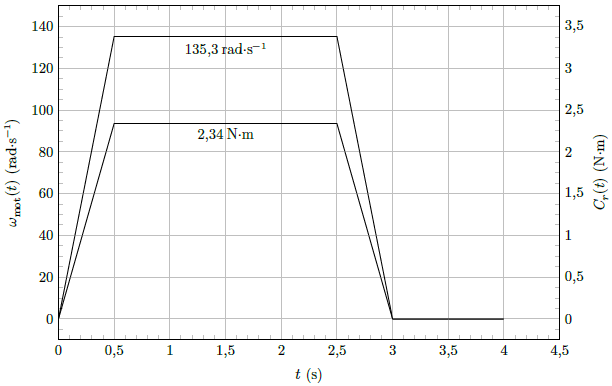
\includegraphics[width=5.35505in,height=3.37736in]{13-MAS-MS/Cours/pandoc/media/image109.png}

\textbf{8.} Le couple résistant peut être assimilé à un couple de frottement visqueux tel que C\textsubscript{r} = K\textsubscript{r}×ω\textsubscript{mot}. \textbf{Déterminer} numériquement la valeur de K\textsubscript{r}.

\textbf{Valeur de réglage du paramètre fréquence du variateur (F\textsubscript{par})}

\ul{Objectif~:} Déterminer la valeur de réglage du paramètre fréquence par une résolution simplifiée.

La résolution rapide consiste à utiliser la partie utile de la caractéristique couple-vitesse de la MAS dont l'expression en fonction du glissement g est la suivante~: \(C_{m} = \frac{p}{\omega} \cdot \frac{3V²}{R} \cdot g\)

\textbf{9. Appliquer} le principe fondamental de la dynamique à l'arbre de la MAS pour établir la relation entre C\textsubscript{m}(t), C\textsubscript{r}(t), ω\textsubscript{mot}(t) et J\textsubscript{e} (J\textsubscript{e}~; moment d'inertie équivalent rapporté sur l'arbre moteur). \textbf{Montrer} qu'en régime permanent (à vitesse constante) C\textsubscript{m}(t) = C\textsubscript{r}(t).

\textbf{10. Exprimer} le glissement g en fonction de f, ω\textsubscript{mot} et p

\textbf{11.} Le variateur de vitesse fonctionne à \(\frac{V}{f}\) constant. À l'aide des expressions précédentes, \textbf{déterminer} la valeur numérique de la pulsation ω des tensions et courants statoriques de la MAS pour que son arbre tourne à 135,3 rad⋅s\textsuperscript{1} en régime établi. \textbf{En déduire} la valeur de réglage du paramètre fréquence du variateur (F\textsubscript{par}). Pour l'application numérique, on prendra R = 9,3 Ω.

\ul{\hfill\break
}

\ul{Objectif~:} Déterminer la valeur de réglage du paramètre fréquence par une résolution numérique.

La résolution numérique consiste à utiliser un programme écrit en langage Python qui va permettre de minimiser la fonction f = C\textsubscript{m}(t) -- C\textsubscript{r}(t) et de tracer sur un même graphe les fonctions C\textsubscript{m}(ω\textsubscript{mot}) et C\textsubscript{r}(ω\textsubscript{mot}), reproduite ci-dessous.

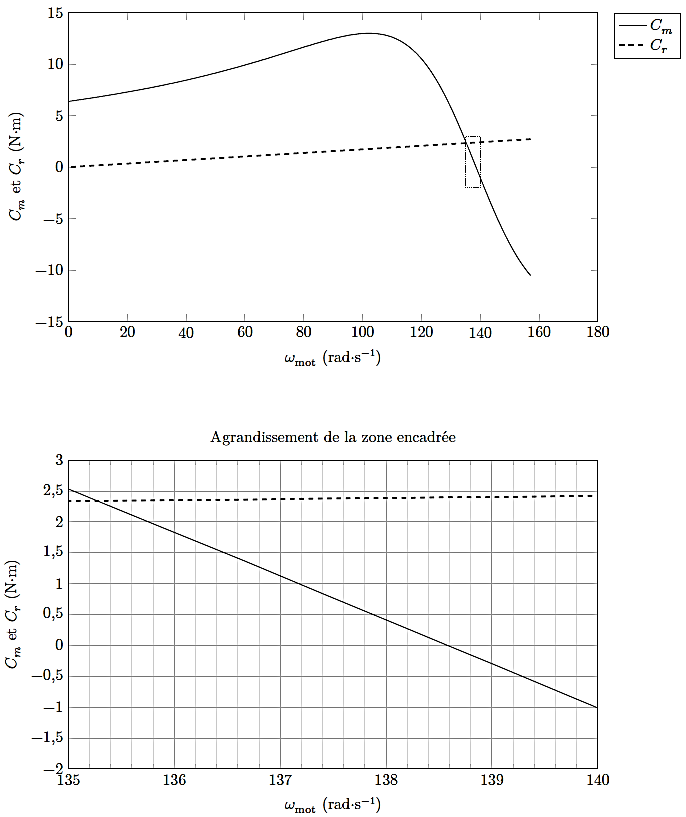
\includegraphics[width=5.15181in,height=2.77358in]{13-MAS-MS/Cours/pandoc/media/image110.png}

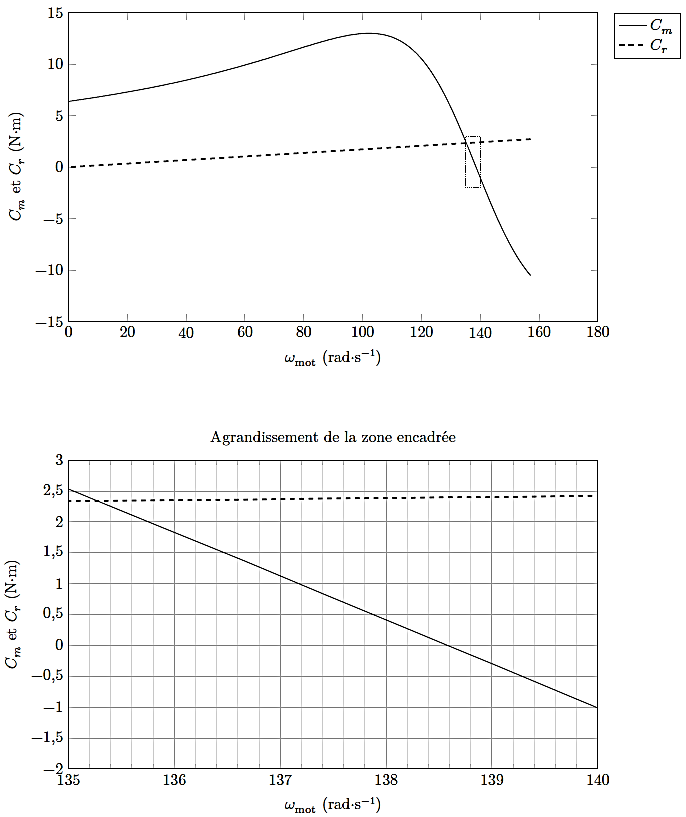
\includegraphics[width=5.19811in,height=3.30189in]{13-MAS-MS/Cours/pandoc/media/image110.png}

\textbf{12.} À l'aide de l'expression de C\textsubscript{max}, \textbf{justifier} l'intérêt de ce type de commande lorsque la fréquence f varie. \textbf{Calculer} pour le point nominal de fonctionnement donné sur la plaque signalétique de la MAS le coefficient \(K_{f} = \frac{V}{f}\).

\textbf{13. Exprimer} le couple C\textsubscript{m} en fonction de K\textsubscript{f}, p, R, L et D\textsubscript{ω} = 2πf -pω\textsubscript{mot}.

\textbf{14.} En exploitant les courbes du générées par le programme, \textbf{indiquer} la valeur de F\textsubscript{par} qu'afficherait le programme.

\textbf{15. Évaluer} les écarts entre les valeurs du paramètre de fréquence F\textsubscript{par} obtenues par la méthode de résolution simplifiée et la méthode de résolution numérique

\textbf{\ul{\hfill\break
}}

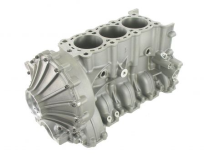
\includegraphics[width=0.92981in,height=0.72642in]{13-MAS-MS/Cours/pandoc/media/image111.png}


\includegraphics[width=1.35556in,height=0.38889in]{13-MAS-MS/Cours/pandoc/media/image77.png}\textbf{DEBOURREUSE DE NOYAUX DE FONDERIE}

\emph{(\ul{Source :} Centrale Supélec TSI 2009)}

\textbf{Mise en situation}

L'entreprise Montupet conçoit, réalise, et produit des culasses pour des moteurs thermiques destinées à équiper les véhicules des grands constructeurs automobiles européens. La culasse compose la partie haute du moteur, elle permettra d'assurer la distribution dans les différents cylindres du mélange air et combustible servant pour la combustion. Les culasses sont réalisées par la technique de fonderie en coquille avec coulée de l'alliage d'aluminium par gravité.


\includegraphics[width=4.63194in,height=3.31042in]{13-MAS-MS/Cours/pandoc/media/image112.emf}Des cavités intérieures réalisées dans la culasse permettent le passage du mélange de combustion et du liquide de refroidissement. La technique de réalisation par fonderie utilisée ici impose l'utilisation d'une coquille en acier, possédant l'empreinte des formes extérieures de la culasse, dans laquelle on positionnera des noyaux en sable pour la réalisation des cavités intérieures.

Pour réaliser la réduction des mottes de noyaux en sable et leur évacuation, de très fortes accélérations sont transmises aux culasses par l'intermédiaire de deux moteurs à balourd (un par culasse provoquant des vibrations indépendantes) liés au support (voir ci-contre). Il est nécessaire de transmettre des accélérations minimales de l'ordre de \textbf{16 m.s\textsuperscript{-2}} à une fréquence comprise entre \textbf{20 et 25 Hz}, pour que les mottes de sable se désagrègent en grains de sable et puissent être mises en mouvement pour sortir des cavités de la culasse.

La présence de deux moteurs permettra d'obtenir une accélération dans le plan horizontal (x,y). Celle-ci sera transmise à l'ensemble mis en mouvement. L'accélération subie par la culasse est issue des effets dus à l'accélération centrifuge imposés par chacun des 2 moteurs à balourd.

Ces actions dynamiques représentent la résultante dynamique générée par la présence des balourds tournant liés au rotor des moteurs. On considère que l'accélération générée est liée directement à la valeur de l'action dynamique imposée par le moteur.

La masse de l'ensemble (2 moteurs, le support, 2 culasses, 4 marteaux et des composants annexes) mis en mouvement par les 2 moteurs à balourd est de \textbf{4940 kg}.

Les caractéristiques techniques des moteurs à balourd sont données sur en annexe. Un seul variateur de vitesse alimente les deux moteurs à balourds. Ces derniers sont du type moteur asynchrone triphasé tétra polaire.

Le rendement des machines asynchrones est de 80\%.

\textbf{1.} Justifier l'utilisation des moteurs à balourds. Justifier l'utilisation de moteurs asynchrones triphasés pour les moteurs à balourds.

\textbf{2.} Calculer la valeur de l'action dynamique nécessaire que chaque moteur à balourd doit générer sur la culasse pour répondre au cahier des charges.

\textbf{3.} À partir de la documentation fournie en annexe, déterminer le moteur à balourd qui répond au mieux aux critères du cahier des charges. Justifier par un simple bilan de puissance le choix d'un variateur de puissance de \textbf{20 kW}.

La cadence de production impose que 2 culasses soient traitées en 90 secondes. La durée pendant laquelle les moteurs à balourd génèrent des accélérations est de \textbf{60 secondes}.

Par conséquent, les phases d'accélération et de décélération des machines asynchrones sont primordiales. On ne s'intéressera ici qu'aux phases de décélération, car elles conditionnent la phase de libération des culasses du support.

On se propose dans un premier temps de vérifier la nécessité d'un dispositif de freinage. Dans un second temps, on analysera 2 modes de freinage, et un choix sur un critère énergétique sera fait. Enfin, dans l'objectif de justifier le choix d'une résistance de freinage et de quantifier l'énergie à dissiper lors des phases de freinage, il sera nécessaire de déterminer les différents paramètres électriques des moteurs à balourds.

\textbf{Nécessité d'un dispositif de freinage}

On se propose dans cette partie de vérifier la nécessité d'un dispositif de freinage. La phase de freinage débute à l'instant où l'alimentation des machines asynchrones est coupée.

On suppose que le moment d'inertie ramené sur l'arbre du moteur vaut \textbf{J = 0,33 kg.m\textsuperscript{2}}, et que le couple résistant est uniquement dû aux frottements visqueux de coefficient estimé à \textbf{f = 5.10\textsuperscript{-2} N.m.s}. Le couple de frottement sec sera négligé.

\textbf{4.} Appliquer le théorème du moment dynamique à l'arbre du moteur durant une phase de freinage et en déduire une équation différentielle liant J, Ω et f.

\textbf{5.} Résoudre cette équation différentielle, en prenant pour origine des temps, l'instant où l'on coupe l'alimentation des machines asynchrones. La vitesse de rotation initiale est prise égale à \textbf{1440 tr.min\textsuperscript{-1}}.

\textbf{6.} En déduire le temps nécessaire aux moteurs asynchrones pour s'arrêter. Le couple de frottement sec ayant été négligé, on considèrera que l'arrêt est obtenu lorsque la vitesse calculée atteint 1\% de la vitesse initiale. Conclure sur la nécessité d'un dispositif de freinage.

\textbf{Expression du couple électromagnétique fourni par une MAS et détermination des paramètres}

Les caractéristiques nominales des machines asynchrones triphasées sont~:

\begin{itemize}
\item
  Puissance nominale \textbf{P\textsubscript{n} = 7,75 kW}
\item
  Courant nominal \textbf{I\textsubscript{n} = 13 A}
\item
  Tension d'alimentation \textbf{230/400 V}
\item
  Fréquence statorique \textbf{f\textsubscript{s} = 50 Hz}
\item
  Vitesse de rotation nominale \textbf{N\textsubscript{n} = 1440 tr.min\textsuperscript{-1}}
\item
  Couplage étoile
\item
  Les tensions et les courants sont considérés alternatifs \textgreater{} parfaitement sinusoïdaux
\end{itemize}


\includegraphics[width=2.62222in,height=1.42569in]{13-MAS-MS/Cours/pandoc/media/image113.emf}On se propose tout d'abord de déterminer l'expression du couple électromagnétique fourni par une machine asynchrone en fonction des paramètres électriques et mécaniques de celle-ci. Le modèle équivalent d'une phase d'une machine asynchrone triphasée équilibrée est donné ci-contre.

On notera \textbf{L} l'inductance magnétisante, \textbf{ℓ\textsubscript{fr}} l'inductance de fuite ramenée au stator, \textbf{R\textsubscript{r}} la résistance rotorique ramenée au stator et \textbf{g} le glissement. De plus, \textbf{Ω\textsubscript{s}} représente la vitesse angulaire du champ tournant statorique exprimée en rad.s\textsuperscript{-1}, et \textbf{ω\textsubscript{s}} la pulsation des grandeurs électriques statoriques en rad.s\textsuperscript{-1}.

\textbf{\hfill\break
}

\textbf{7.} Déterminer le nombre de paires de pôles \textbf{p} des machines asynchrones.

\textbf{8.} Déterminer l'expression de la puissance transmise au rotor pour une machine asynchrone en fonction de ℓ\textsubscript{fr}, R\textsubscript{r}, g, ω\textsubscript{s} et V\textsubscript{s}.

\textbf{9.} En déduire l'expression du couple électromagnétique \textbf{C} fourni par une machine asynchrone en fonction de ℓ\textsubscript{fr}, R\textsubscript{r}, g, p, Ω\textsubscript{s} et V\textsubscript{s}.

Afin de caractériser les machines asynchrones triphasées, il est nécessaire d'identifier les différents paramètres du modèle monophasé. Pour cela, deux essais ont été réalisés~:

\begin{itemize}
\item
  1\textsuperscript{er} essai~: Essai à la vitesse angulaire de synchronisme Ω\textsubscript{s} sous \textgreater{} une tension entre Phase et Neutre de \textbf{230 V} à la fréquence de \textgreater{} \textbf{50 Hz}. La puissance réactive absorbée par une machine \textgreater{} asynchrone triphasée vaut \textbf{800 VAR}.
\item
  2\textsuperscript{nd} essai~: Essai à rotor calé (= 0) sous tension réduite. Une \textgreater{} machine asynchrone triphasée est alimentée par une source de \textgreater{} tension triphasée délivrant une tension simple de valeur efficace \textgreater{} prise égale à \textbf{V\textsubscript{cc} = 76 V}, la valeur efficace du courant \textgreater{} absorbé par phase est \textbf{I\textsubscript{cc}} et vaut \textbf{13 A}. Dans ces \textgreater{} conditions, une machine asynchrone triphasée absorbe une puissance \textgreater{} active \textbf{P\textsubscript{cc} = 350 W}.
\end{itemize}

\textbf{10.} Avec l'essai 1~:

\begin{itemize}
\item
  Quelle est la valeur du glissement pour cet essai~?
\item
  Après avoir exprimé la puissance réactive absorbée par la machine \textgreater{} asynchrone pour l'essai 1, déterminer la valeur de l'inductance \textgreater{} magnétisante \textbf{L}.
\end{itemize}

\textbf{11.} Avec l'essai 2~:

\begin{itemize}
\item
  Justifier que l'essai à rotor bloqué soit réalisé sous tension \textgreater{} réduite.
\item
  Quelle est la valeur du glissement pour cet essai~?
\item
  Déterminer la valeur efficace du courant \textbf{I\textsubscript{r}}.
\item
  Déterminer les valeurs de la résistance \textbf{R\textsubscript{r}} et de l'inductance \textgreater{} de fuite \textbf{ℓ\textsubscript{fr}}.
\end{itemize}

Pour la suite du sujet, on prendra \textbf{R\textsubscript{r} = 730 mΩ}~; \textbf{L = 630 mH} et \textbf{ℓ\textsubscript{fr} = 20 mH}.

\textbf{12.} Déterminer l'expression numérique du couple électromagnétique \textbf{C} en fonction du glissement g pour \textbf{f\textsubscript{s} =50Hz}. En déduire la valeur du couple maximum et la valeur du glissement pour laquelle on l'atteint.

\textbf{13.} Tracer l'allure de la courbe du couple électromagnétique \textbf{C} en fonction du glissement g pour g∈{[}-1;1{]}.

\textbf{14.} Préciser les modes de fonctionnement (moteur ou frein) de la machine asynchrone triphasée en fonction de la valeur du glissement g.

\textbf{ANNEXE~: Documentation technique des moteurs à balourd}

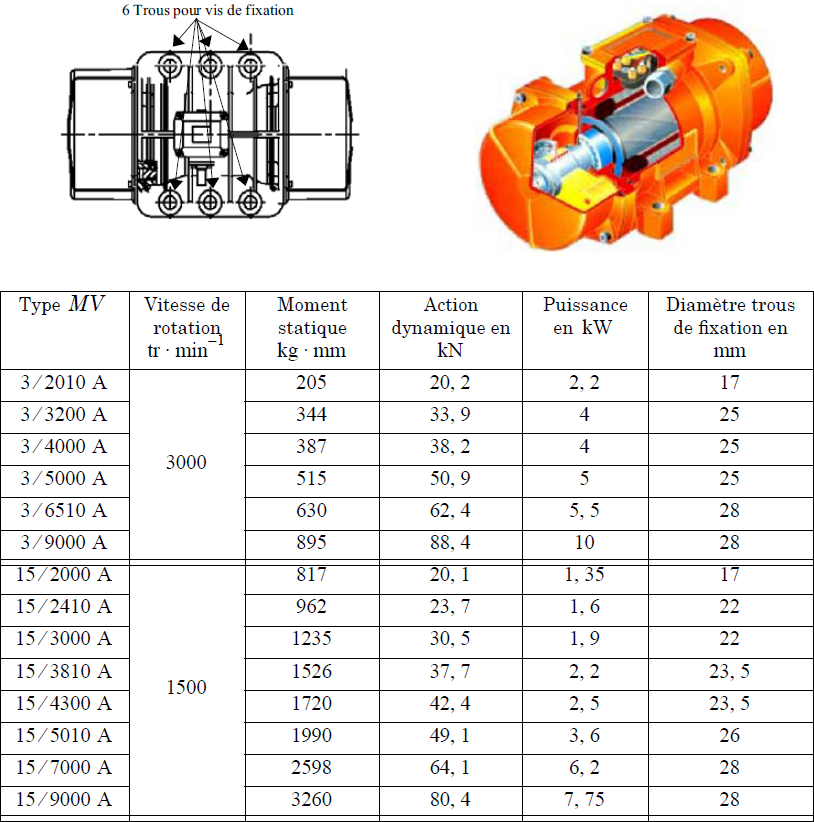
\includegraphics[width=6.75591in,height=6.82677in]{13-MAS-MS/Cours/pandoc/media/image114.png}

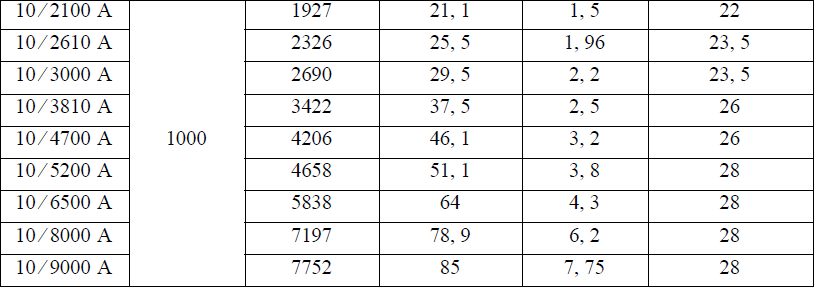
\includegraphics[width=6.75591in,height=2.38583in]{13-MAS-MS/Cours/pandoc/media/image115.png}

\textbf{\ul{\hfill\break
}}

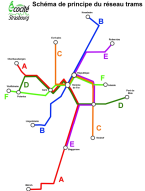
\includegraphics[width=0.65823in,height=0.86792in]{13-MAS-MS/Cours/pandoc/media/image116.png}\textbf{TRAMWAY DE STRASBOURG}


\includegraphics[width=1.35556in,height=0.38889in]{13-MAS-MS/Cours/pandoc/media/image77.png} \emph{(\ul{Source :} Concours 3ème année ENS Cachan 2002)}

\textbf{Mise en situation}

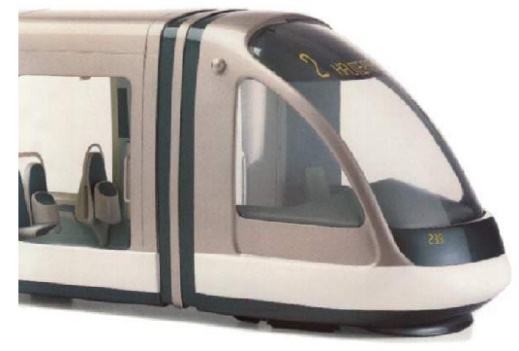
\includegraphics[width=2.36389in,height=1.59583in]{13-MAS-MS/Cours/pandoc/media/image117.jpeg}Une rame de tramway de Strasbourg se compose de quatre bogies dont trois sont moteurs. Un bogie moteur est composé de quatre roues entraînées chacune par un moteur asynchrone triphasé par l'intermédiaire d'un réducteur. Une rame de tramway est donc motorisée par douze moteurs asynchrones.

\textbf{\ul{Principe de traction}}

Le schéma de traction retenu pour le Tramway de Strasbourg est donné ci-dessous. Chaque onduleur de traction alimente deux des quatre machines asynchrones placées sur chaque bogie. Cette commande indépendante des roues situées à droite et à gauche du bogie permet d\textquotesingle améliorer les passages en courbe.

Le conducteur, par l'intermédiaire d'une manette, peut moduler l'effort de traction à appliquer à la rame de tramway. Ceci revient à moduler le couple électromagnétique des moteurs. Le constructeur a choisi d'implanter une commande permettant d'imposer le couple électromagnétique instantané sur l'arbre des moteurs.

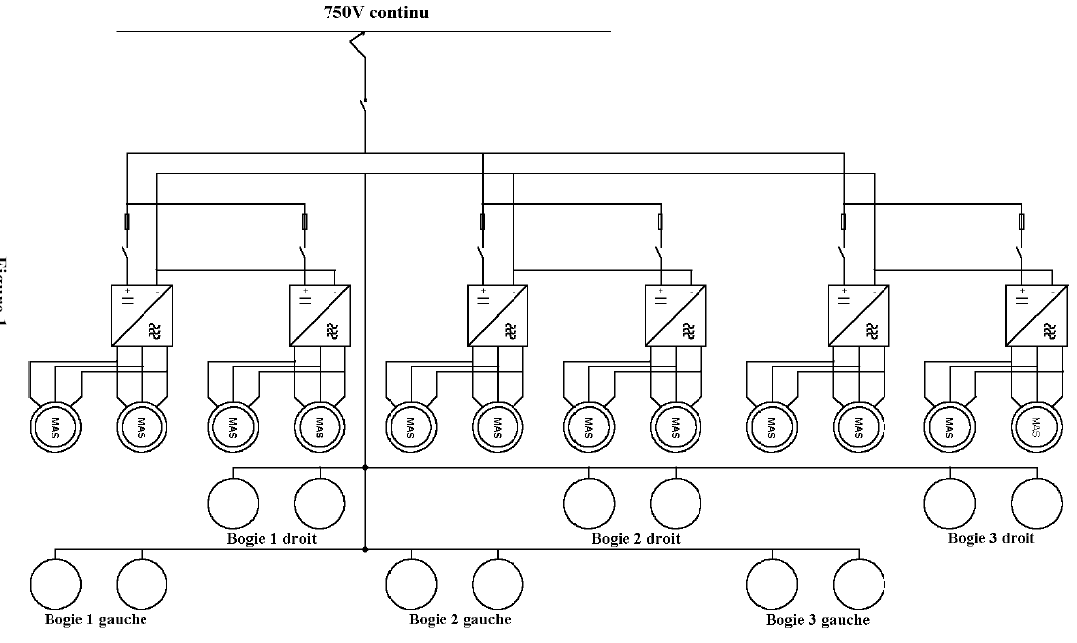
\includegraphics[width=6.4583in,height=3.83782in]{13-MAS-MS/Cours/pandoc/media/image118.png}

\textbf{\ul{Caractéristiques nominales du moteur}}

Il s\textquotesingle agit d\textquotesingle un moteur asynchrone triphasé à rotor à cage dont les enroulements statoriques sont couplés en étoile.

\begin{itemize}
\item
  Tension nominale entre phases~: U\textsubscript{N} = 585 V
\item
  Fréquence statorique nominale~: f\textsubscript{N} = 88 Hz
\item
  Intensité nominale du courant statorique~: l\textsubscript{N} = 35,4 A
\item
  Facteur de puissance nominal~: cos ϕ\textsubscript{N} = 0,732
\item
  Fréquence nominale de synchronisme~: N\textsubscript{s} = 2640 tr.min\textsuperscript{-1}
\item
  Fréquence nominale de rotation du rotor~: N\textsubscript{N} = 2610 tr.min\textsuperscript{-1}
\end{itemize}

Dans ce qui suit, on néglige~: Les résistances et inductances de fuites statoriques

Les pertes dans le fer

Les pertes mécaniques

\textbf{Etude du fonctionnement nominal du moteur}

\textbf{1.} Déterminer le nombre p de paires de pôles du moteur.

\textbf{2.} Calculer le glissement g\textsubscript{N}.

\textbf{3.} Calculer la puissance électrique P\textsubscript{N} absorbée par le moteur et préciser la valeur de la puissance électromagnétique P\textsubscript{TrN} transmise au rotor.

\textbf{4.} Calculer le couple électromagnétique C\textsubscript{N}.

\textbf{5.} Exprimer les pertes par effet Joule au rotor P\textsubscript{Jr} en fonction de P\textsubscript{Tr}. Calculer P\textsubscript{JrN}.

\textbf{6.} Calculer la puissance utile P\textsubscript{UN} développée par le moteur.

\textbf{Fonctionnement dans les quatre quadrants}

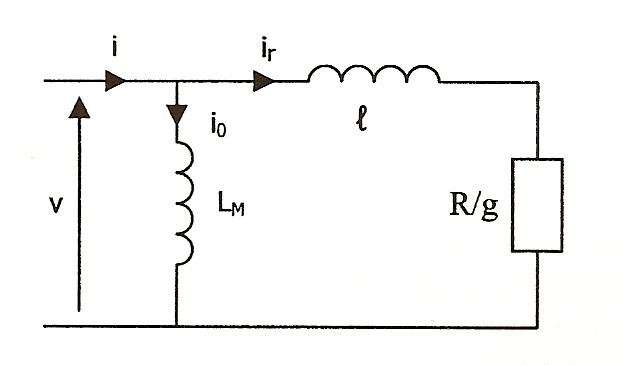
\includegraphics[width=2.58264in,height=1.51111in]{13-MAS-MS/Cours/pandoc/media/image119.png}L\textquotesingle association du convertisseur et de la motorisation doit permettre le fonctionnement de la machine asynchrone dans les 4 quadrants mécaniques c\textquotesingle est-à-dire pour le Tramway de Strasbourg, la circulation dans les deux sens de marche et le freinage électrique. Les tensions alimentant la machine asynchrone sont sinusoïdales triphasées (v\textsubscript{AN}, v\textsubscript{BN} et v\textsubscript{CN}) et que le modèle équivalent par phase de la machine peut être assimilé au schéma simplifié ci-dessous.

\begin{itemize}
\item
  R/g est la résistance modélisant le transfert de puissance active au \textgreater{} rotor
\item
  L\textsubscript{M} est l'inductance magnétisante
\item
  L\textsubscript{t} est l'inductance totale de fuites vue du stator
\item
  g est le glissement
\item
  v est une tension simple du réseau d'alimentation de valeur efficace \textgreater{} V (v = v\textsubscript{xN} avec x = A, B ou C)
\item
  i est l'intensité en ligne.
\end{itemize}

On donne~: R = 0,138 Ω L\textsubscript{t} = 2,38 mH L\textsubscript{M} = 26,55 mH.


\includegraphics{13-MAS-MS/Cours/pandoc/media/image120.wmf}\textbf{7.} Déterminer l\textquotesingle expression du couple électromagnétique C en fonction de V, L\textsubscript{t}, R, g, p et ω (pulsation des grandeurs statoriques). Mettre le résultat sous la forme ci-contre en précisant les expressions de A et de g\textsubscript{0}.

On prendra pour les applications numériques suivantes~: V = 338 V et f = 88 Hz.

\textbf{8.} Pour quelle valeur de g, le couple est-il maximal~? Déterminer alors le couple maximal C\textsubscript{MAX}. Effectuer les applications numériques.

\textbf{9.} Tracer la caractéristique C(N) d'un moteur de traction pour 0 \textless{} N \textless{} 2N\textsubscript{s} avec N en tr/min. Préciser les points remarquables, la partie stable de la caractéristique ainsi que les plages de fonctionnement en moteur et en génératrice.

\textbf{10.} En précisant l'hypothèse faite, montrer que la caractéristique de couple peut se mettre sous la forme C ≈ K.g avec K = 8972 Nm. Représenter cette caractéristique approchée sur le graphe précédent.

\textbf{11.} En utilisant le résultat de la question précédente, calculer le glissement puis la vitesse de rotation du moteur N (en tr/min) pour C = 90 Nm puis pour C = -90 Nm.

\textbf{12.} On souhaite inverser le sens de rotation des moteurs de traction pour effectuer une marche arrière. Comment procède-t-on~?

\textbf{13.} Représenter, sur le document réponse, les tensions v\textsubscript{BN} et v\textsubscript{CN} nécessaires pour aller dans les différents quadrants de fonctionnement du moteur. Les conventions sont données pour le quadrant 1. Préciser pour chaque quadrant le type de fonctionnement de la machine.

\textbf{14.} Montrer que l\textquotesingle expression du déphasageϕ de v par rapport à i est donnée par~:

\begin{quote}

\includegraphics{13-MAS-MS/Cours/pandoc/media/image121.wmf}
\end{quote}

\textbf{15.} En déduire les valeurs de ϕ pour C = 90 Nm puis pour C = -90 Nm. Commenter les résultats obtenus.

\textbf{16.} Compléter le document réponse en représentant les courants i\textsubscript{A}, i\textsubscript{B}, i\textsubscript{C} dans chacun des 4 quadrants mécaniques permettant d'obtenir un couple en valeur absolue de 90 Nm.

\textbf{DOCUMENT RÉPONSE}

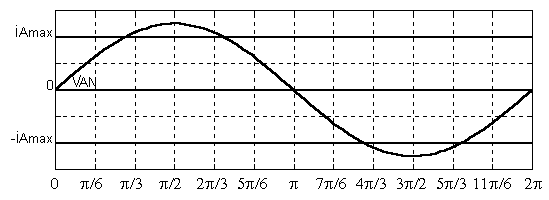
\includegraphics[width=7.45625in,height=9.42361in]{13-MAS-MS/Cours/pandoc/media/image123.png}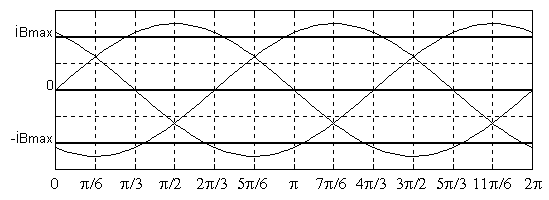
\includegraphics[width=7.45625in,height=9.42361in]{13-MAS-MS/Cours/pandoc/media/image124.png}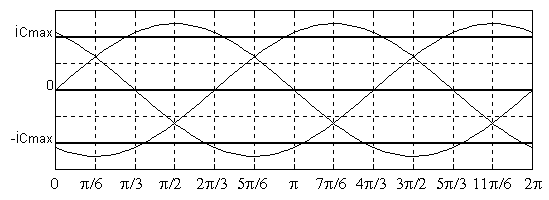
\includegraphics[width=7.45625in,height=9.42361in]{13-MAS-MS/Cours/pandoc/media/image125.png}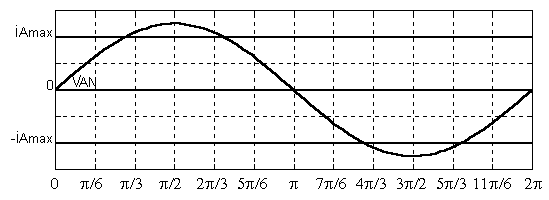
\includegraphics[width=7.45625in,height=9.42361in]{13-MAS-MS/Cours/pandoc/media/image123.png}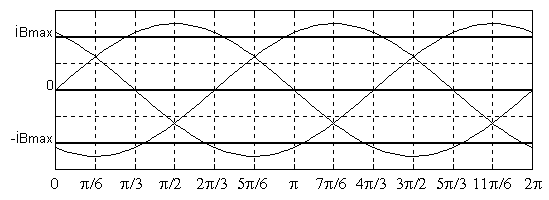
\includegraphics[width=7.45625in,height=9.42361in]{13-MAS-MS/Cours/pandoc/media/image124.png}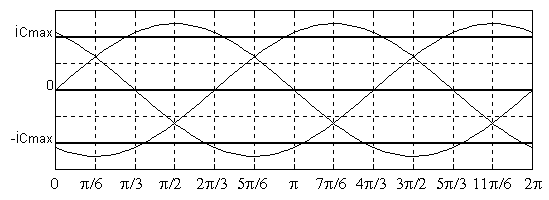
\includegraphics[width=7.45625in,height=9.42361in]{13-MAS-MS/Cours/pandoc/media/image125.png}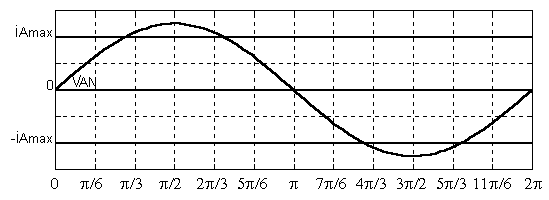
\includegraphics[width=7.45625in,height=9.42361in]{13-MAS-MS/Cours/pandoc/media/image123.png}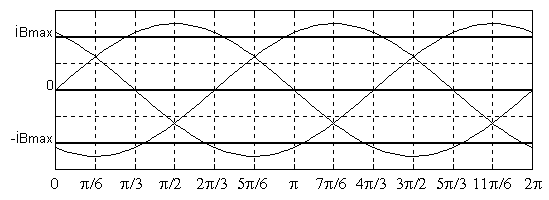
\includegraphics[width=7.45625in,height=9.42361in]{13-MAS-MS/Cours/pandoc/media/image124.png}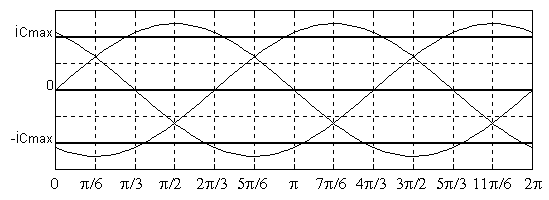
\includegraphics[width=7.45625in,height=9.42361in]{13-MAS-MS/Cours/pandoc/media/image125.png}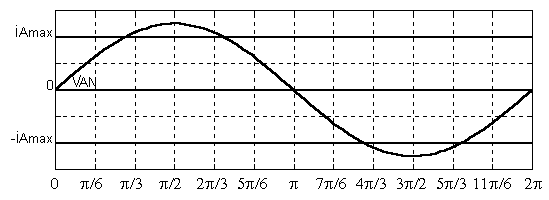
\includegraphics[width=7.45625in,height=9.42361in]{13-MAS-MS/Cours/pandoc/media/image123.png}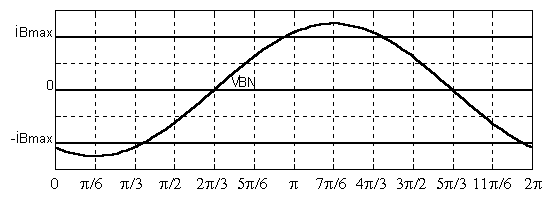
\includegraphics[width=7.45625in,height=9.42361in]{13-MAS-MS/Cours/pandoc/media/image126.png}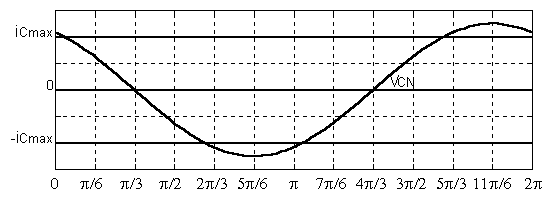
\includegraphics[width=7.45625in,height=9.42361in]{13-MAS-MS/Cours/pandoc/media/image127.png}


\includegraphics[width=1.35556in,height=0.38889in]{13-MAS-MS/Cours/pandoc/media/image77.png}

\textbf{TABLE DE RADIOLOGIE D²RS}

\emph{(\ul{Source} : ATS 2018)}

\textbf{Mise en situation}

\ul{Présentation du système}

La table de radiologie D²RS (Digital Dynamic Remote System) conçue et commercialisée par STEPHANIX répond aux fonctions suivantes~:

\begin{itemize}
\item
  supporter et positionner le patient ainsi que le système d'imagerie
\item
  intégrer de nouveaux critères d'innovation~:
\end{itemize}

\begin{itemize}
\item
  dernière génération de capteur plan dynamique
\item
  positionnement automatique en fonction du protocole sélectionné
\end{itemize}

\begin{itemize}
\tightlist
\item
  réaliser des tomosynthèses* (pseudo 3D, protocole de détection \textgreater{} précoce de certains cancers) grâce à l'interpolation de 2 axes en \textgreater{} mouvement.
\end{itemize}


\includegraphics[width=4.31961in,height=3.5283in]{13-MAS-MS/Cours/pandoc/media/image128.emf}

*La tomosynthèse est une technique d'imagerie radiologique ancienne et tombée en désuétude qui redevient d'actualité grâce au développement des technologies numériques de traitement d'images radiologiques. À partir d'une table radiologique classique, elle permet dorénavant une acquisition volumique (dite pseudo-3D) de la zone observée.

\ul{Problématique}

Lorsque le manipulateur radio agit sur le mouvement de chariotage pour positionner précisément la source de rayons X et cibler la zone à radiographier pour une tomosynthèse, des instabilités apparaissent à basse vitesse et perturbent son réglage.

\textbf{Détermination des grandeurs nominales de la machine}

\ul{Hypothèses~:}

La table de radiographie D²RS est alimentée par le réseau triphasé 400 V / 50 Hz. Toutes les pertes de la machine asynchrone sont négligées à l'exception des pertes joules au rotor et des pertes mécaniques.

\textbf{1. Prendre} connaissance de la plaque signalétique en annexe. \textbf{Déterminer} alors pour cette machine~:

\begin{itemize}
\item
  le couplage des enroulements
\item
  le nombre de paires de pôles p
\item
  le glissement nominal g\textsubscript{n}
\item
  la puissance active absorbée nominale P\textsubscript{ab}
\item
  les pertes joules rotoriques P\textsubscript{jr}
\item
  les pertes mécaniques P\textsubscript{pm}
\item
  le rendement nominal η\textsubscript{n}
\end{itemize}

\ul{Modèle équivalent par phase de la machine asynchrone~:}

Réactance de magnétisation X\textsubscript{m} = L\textsubscript{m}.ω

Réactance de fuite d'une phase rotor ramenée au stator X\textsubscript{2} = L\textsubscript{2}.ω

Résistance d'une phase rotor ramenée au stator R\textsubscript{2}

Glissement g

Pulsation des courants statoriques ω

Deux essais ont été effectués pour déterminer les valeurs numériques des paramètres~:

\begin{longtable}[]{@{}
  >{\raggedright\arraybackslash}p{(\columnwidth - 2\tabcolsep) * \real{0.4444}}
  >{\raggedright\arraybackslash}p{(\columnwidth - 2\tabcolsep) * \real{0.5417}}@{}}
\toprule\noalign{}
\begin{minipage}[b]{\linewidth}\raggedright
Essai à vide
\end{minipage} & \begin{minipage}[b]{\linewidth}\raggedright
\end{minipage} \\
\midrule\noalign{}
\endhead
\bottomrule\noalign{}
\endlastfoot
Conditions de l'essai & Mesures \\
Machine désaccouplée

Tension d'alimentation V\textsubscript{10} = 230 V

Fréquence f = 50 Hz & Puissance réactive absorbée Q\textsubscript{0} = 1322 VAR \\
\end{longtable}

\begin{longtable}[]{@{}
  >{\raggedright\arraybackslash}p{(\columnwidth - 2\tabcolsep) * \real{0.4444}}
  >{\raggedright\arraybackslash}p{(\columnwidth - 2\tabcolsep) * \real{0.5417}}@{}}
\toprule\noalign{}
\begin{minipage}[b]{\linewidth}\raggedright
Essai à rotor bloqué
\end{minipage} & \begin{minipage}[b]{\linewidth}\raggedright
\end{minipage} \\
\midrule\noalign{}
\endhead
\bottomrule\noalign{}
\endlastfoot
Conditions de l'essai & Mesures \\
Machine avec rotor bloqué

Tension d'alimentation V\textsubscript{1rb} = 15 V

Fréquence f = 50 Hz & Puissance apparente absorbée S\textsubscript{rb} = 245 VA

Intensité du courant I\textsubscript{2rb} = 2,49 A

Facteur de puissance f\textsubscript{p} = 0,69 \\
\end{longtable}

\textbf{2. Faire} une hypothèse sur la valeur du glissement dans l'essai à vide et \textbf{représenter} le schéma simplifié du modèle équivalent par phase. \textbf{Exprimer} la puissance réactive Q\textsubscript{0} en fonction des éléments du schéma et \textbf{en déduire} la valeur numérique de l'inductance de magnétisation L\textsubscript{m}.

\textbf{3. Faire} une hypothèse sur la valeur du glissement dans l'essai à rotor bloqué et \textbf{représenter} le schéma simplifié du modèle équivalent par phase\textbf{. Exprimer} les puissances active P\textsubscript{rb} et réactive Q\textsubscript{rb} en fonction des éléments du schéma. \textbf{En déduire} les valeurs numériques de la résistance rotorique R\textsubscript{2} et de l'inductance de fuite rotorique L\textsubscript{2}.

Les valeurs numériques retenues pour la suite du problème sont~:

\begin{quote}
Inductance de magnétisation L\textsubscript{m} = 0,382 H

Inductance de fuite d'une phase rotor ramenée au stator L\textsubscript{2} = 29,4 mH

Résistance d'une phase rotor ramenée au stator R\textsubscript{2} = 9,08 Ω
\end{quote}

\textbf{4. Indiquer} le paramètre de l'alimentation sur lequel on peut agir pour faire varier la vitesse de la machine.

\textbf{5. Montrer} que le couple électromagnétique de la machine peut se mettre sous la forme \(C_{em} = K.\frac{x}{(x^{2} + X_{2}^{2})}\ \) et \textbf{exprimer} les paramètres K et x. \textbf{Valider} le modèle par le calcul du couple nominal de la machine. Puis \textbf{montrer} que C\textsubscript{em} est maximum pour \(g = g_{\max} = \frac{R_{2}}{X_{2}}\). \textbf{En déduire} l'expression de C\textsubscript{max} en fonction de L\textsubscript{2}, V\textsubscript{1}, p et f.

\textbf{6. Justifier} qualitativement le choix d'une commande scalaire en \(\frac{V_{1}}{f}\) pour une machine asynchrone associée à un onduleur de tension (ou de courant).

\textbf{Etude de la commande scalaire}

Le couple dans une machine asynchrone est directement proportionnel au carré du flux créé par l'inductance magnétisante L\textsubscript{m}. Les performances optimales sont obtenues si le flux, donc le courant magnétisant \ul{I}\textsubscript{m}, est maintenu constant sur toute la plage de vitesse.

\textbf{7. Exprimer} la valeur efficace du courant magnétisant I\textsubscript{m} en fonction de V\textsubscript{1}, L\textsubscript{m} et f, puis \textbf{justifier} le choix d'une commande scalaire.

Un modèle plus complet de la machine asynchrone est proposé ci-dessous.

Réactance de magnétisation X\textsubscript{m} = L\textsubscript{m}.ω

Réactance de fuite d'une phase rotor ramenée au stator X\textsubscript{2} = L\textsubscript{2}.ω

Résistance d'une phase rotor ramenée au stator R\textsubscript{2}

Réactance de fuite d'une phase stator X\textsubscript{1} = L\textsubscript{1}.ω

Résistance d'une phase stator R\textsubscript{1}

Les paramètres de l'enroulement stator ont fait l'objet d'une mesure. On a relevé R\textsubscript{1} = 0,85 Ωet L\textsubscript{1} = 3,24 mH.

\textbf{8. Calculer} la chute de tension statorique au point nominal.

Par simulation du modèle complet par phase, deux courbes ont été obtenues~: le courant magnétisant I\textsubscript{m}(A) à la figure de gauche et la chute de tension ∆u (\% de V\textsubscript{1}) à la figure de droite, en fonction de la fréquence d'alimentation f (Hz).

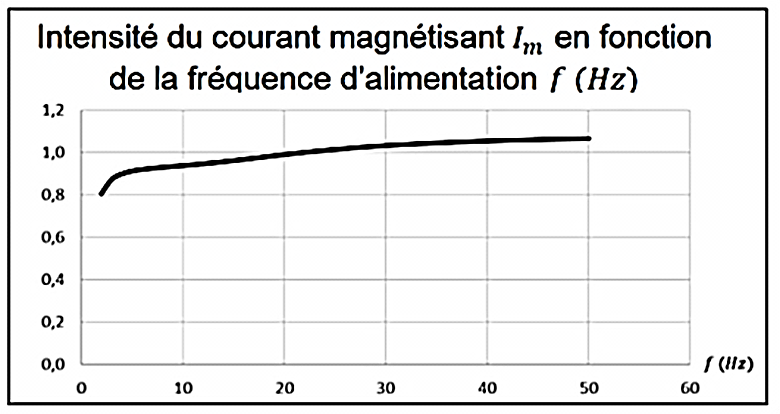
\includegraphics[width=3.58491in,height=1.90371in]{13-MAS-MS/Cours/pandoc/media/image130.png}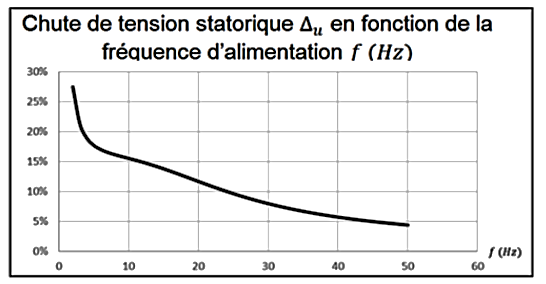
\includegraphics[width=3.64531in,height=1.91925in]{13-MAS-MS/Cours/pandoc/media/image131.png}

\textbf{9. Commenter} les courbes obtenues par simulation et \textbf{conclure} sur les limites de la commande scalaire. \textbf{Proposer} une autre stratégie de commande qui réponde à la problématique.

\ul{Plaque signalétique du moteur~:}

\begin{longtable}[]{@{}
  >{\raggedright\arraybackslash}p{(\columnwidth - 12\tabcolsep) * \real{0.5235}}
  >{\raggedright\arraybackslash}p{(\columnwidth - 12\tabcolsep) * \real{0.1477}}
  >{\raggedright\arraybackslash}p{(\columnwidth - 12\tabcolsep) * \real{0.0537}}
  >{\raggedright\arraybackslash}p{(\columnwidth - 12\tabcolsep) * \real{0.0872}}
  >{\raggedright\arraybackslash}p{(\columnwidth - 12\tabcolsep) * \real{0.0537}}
  >{\raggedright\arraybackslash}p{(\columnwidth - 12\tabcolsep) * \real{0.0604}}
  >{\raggedright\arraybackslash}p{(\columnwidth - 12\tabcolsep) * \real{0.0604}}@{}}
\toprule\noalign{}
\begin{minipage}[b]{\linewidth}\raggedright

\includegraphics[width=0.77165in,height=0.49606in]{13-MAS-MS/Cours/pandoc/media/image132.emf} 
\includegraphics[width=2.13208in,height=0.4973in]{13-MAS-MS/Cours/pandoc/media/image133.emf} 
\includegraphics[width=0.77165in,height=0.49606in]{13-MAS-MS/Cours/pandoc/media/image134.emf}
\end{minipage} & \begin{minipage}[b]{\linewidth}\raggedright
\end{minipage} & \begin{minipage}[b]{\linewidth}\raggedright
\end{minipage} & \begin{minipage}[b]{\linewidth}\raggedright
\end{minipage} & \begin{minipage}[b]{\linewidth}\raggedright
\end{minipage} & \begin{minipage}[b]{\linewidth}\raggedright
\end{minipage} & \begin{minipage}[b]{\linewidth}\raggedright
\end{minipage} \\
\midrule\noalign{}
\endhead
\bottomrule\noalign{}
\endlastfoot
3∼ Mot & M 2SB 4 FD & Cod & 8G360209CV & & & \\
No & F-01-13 / 6771243 & S 1 & IMB & 5 & 14.5 & kg \\
kW & 1.1 / 50 Hz & & & & & \\
Hz & V (+/- 10\%) & A & & min-1 & cosɸ & \\
50 & 230 / 400 D/Y & 4.7 / 2.7 & & 1400 & 0.78 & \\
\end{longtable}

\ul{Extrait du catalogue moteur Bonfiglioli~:}


\includegraphics[width=7.26415in,height=3.87417in]{13-MAS-MS/Cours/pandoc/media/image135.emf}

Avec~: M\textsubscript{a} couple d'accélération moyen (Nm)

M\textsubscript{n} couple nominal (Nm)

M\textsubscript{s} couple de démarrage (Nm)

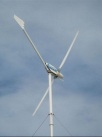
\includegraphics[width=0.4654in,height=0.625in]{13-MAS-MS/Cours/pandoc/media/image136.jpeg}\textbf{EOLIENNE}


\includegraphics[width=1.35556in,height=0.38889in]{13-MAS-MS/Cours/pandoc/media/image77.png} \emph{(\ul{Source} : CAPET SII 2010)}

\textbf{Mise en situation}

Cette installation est implantée dans un camping situé en bordure de l'étang de Thau sur la commune de Mèze (Hérault, 34).

Le propriétaire qui souhaite afficher une démarche respectueuse de l'environnement et réduire sa facture énergétique a exprimé les contraintes suivantes~:

\begin{itemize}
\item
  Un minimum de nuisances sonores pour les campeurs et le propriétaire
\item
  Une installation capable de couvrir au minimum la totalité de la \textgreater{} facture énergétique pour le logement privé, soit une puissance \textgreater{} minimale de 5 kW lors du fonctionnement à la fréquence de rotation \textgreater{} nominale.
\end{itemize}

Les conditions météorologiques retenues sont~:

\begin{itemize}
\item
  Vent local moyen de 10 m/s du secteur EST avec des maximas pouvant \textgreater{} atteindre 27 m/s
\item
  Altitude~: niveau de la mer.
\end{itemize}

Le propriétaire du camping a contacté la société TRAVERE Industries pour réaliser son projet d'implantation d\textquotesingle éolienne.

\textbf{Schéma de l'installation proposée par la société TRAVERE Industries SAS}

Un ensemble redresseur / convertisseur met en forme l'énergie électrique délivrée par l'éolienne pour la renvoyer au réseau électrique BT (Basse Tension). Un compteur d'énergie à courbe de charge calcule l'énergie consommée et l'énergie renvoyée vers le réseau EDF. L'installation électrique du propriétaire est reliée au réseau électrique BT en monophasé.

\textbf{Vérification de la puissance générée}

Le schéma équivalent monophasé pour une phase de la génératrice est représenté ci-dessous.

Pour une vitesse nominale de 240 tr/min la génératrice débite un courant I de 8,38 A avec un déphasage ϕ entre I et V\textsubscript{1} de 18°. La f.é.m. \ul{E} est alors une tension sinusoïdale de fréquence f = 48 Hz, et de valeur efficace E = 311 V.

\textbf{1. Donner} l'expression de \ul{V}\textsubscript{1} en fonction de \ul{I}, \ul{E}, r\textsubscript{1}, ω, et L\textsubscript{1}.

\textbf{2. Déterminer} graphiquement, sur le graphique ci-après, la valeur efficace de la tension \ul{V}\textsubscript{1}.

\textbf{3. Calculer} la puissance active P\textsubscript{gén} fournie par la génératrice pour le fonctionnement nominal. \textbf{En déduire} s'il est possible de couvrir les besoins énergétiques du site de Mèze avec l'installation proposée.

\textbf{4. Conclure}, en indiquant le rendement de la génératrice pour le fonctionnement nominal de l'éolienne TA6-5500 sachant que la puissance mécanique récupérée est de 6,1 kW.

\begin{center}\rule{0.5\linewidth}{0.5pt}\end{center}

\begin{center}\rule{0.5\linewidth}{0.5pt}\end{center}


\includegraphics[width=1.35556in,height=0.38889in]{13-MAS-MS/Cours/pandoc/media/image77.png}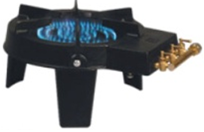
\includegraphics[width=0.9434in,height=0.61043in]{13-MAS-MS/Cours/pandoc/media/image137.png}\textbf{MLPS~: Système automatisé de conditionnement de cartons}

\emph{(\ul{Source} : ATS 2016)}

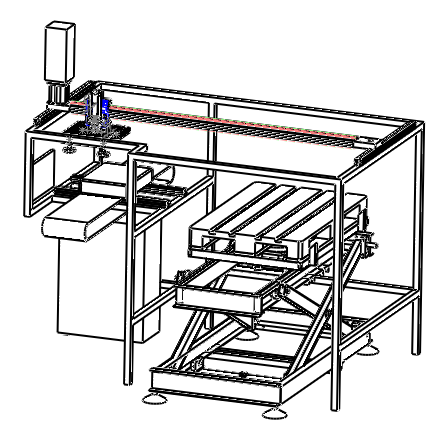
\includegraphics[width=2.65069in,height=2.62014in]{13-MAS-MS/Cours/pandoc/media/image138.png}\textbf{Mise en situation}

Le système MPLS (pour Multi Level Packaging System) permet d\textquotesingle agencer les cartons sur la palette. Ses principaux éléments constitutifs sont~:

\begin{itemize}
\item
  Une \textbf{unité en U,} composée d\textquotesingle un axe numérique et d'un préhenseur \textgreater{} à ventouses, permet la saisie, l\textquotesingle élévation, la translation, la \textgreater{} descente et la dépose d\textquotesingle un carton à une position précise sur la \textgreater{} palette.
\item
  Une \textbf{table élévatrice} permet de descendre la palette de la \textgreater{} hauteur d\textquotesingle un carton quand une couche est terminée.
\item
  Un \textbf{plateau indexeur} permet de faire tourner la palette par pas \textgreater{} de 90° dans le sens horaire et en fonction des besoins du cycle.
\end{itemize}

La production du couple mécanique nécessaire à l\textquotesingle entraînement du préhenseur est assurée par un ensemble moteur synchrone et onduleur de tension à commande MLI.

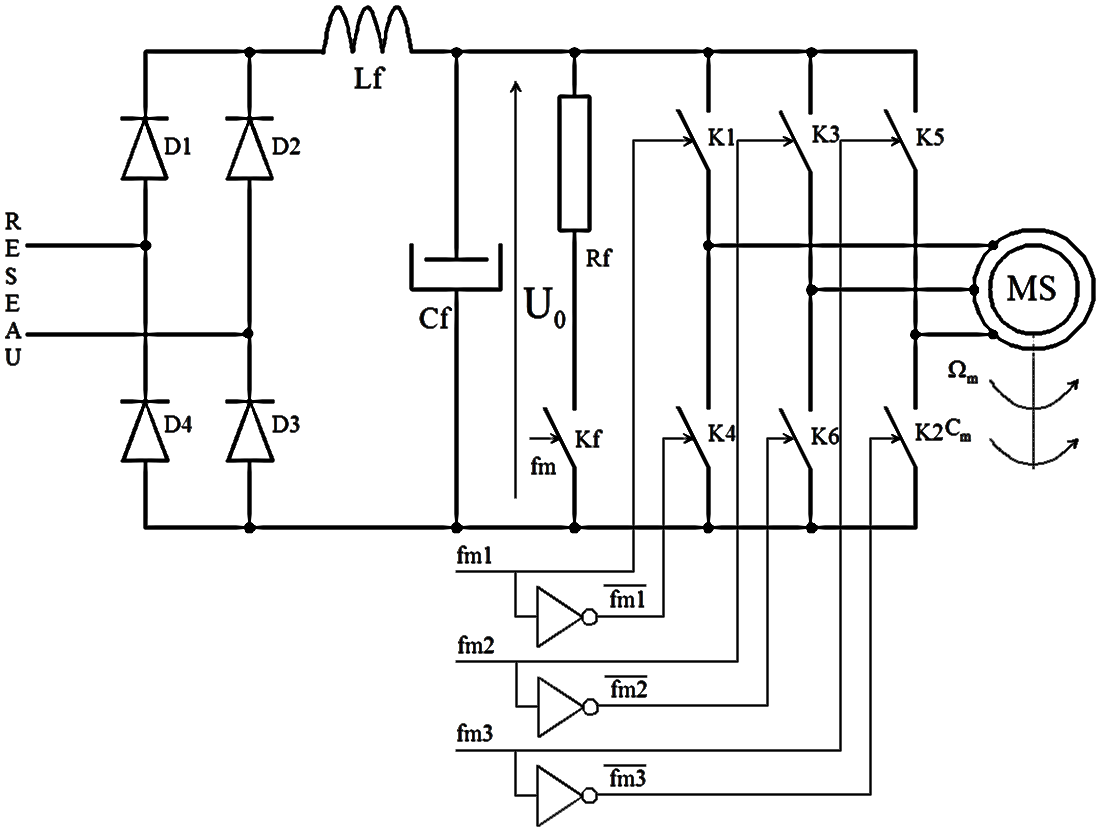
\includegraphics[width=5.30139in,height=4in]{13-MAS-MS/Cours/pandoc/media/image139.png}La machine synchrone est alimentée depuis le réseau EDF 230V/50Hz par la chaîne d\textquotesingle énergie dont le schéma de principe est représenté ci-dessous~:

Le rôle de l\textquotesingle ensemble redresseur à diodes D1 à D4 et filtre Lf / Cf est de convertir le réseau sinusoïdal d\textquotesingle EDF en une source de tension U\textsubscript{0} que l\textquotesingle on supposera continue.

Le rôle de l\textquotesingle ensemble convertisseur à trois cellules de commutation (K1/K4 ; K3/K6 ; K5/K2) est de convertir la source de tension continue U\textsubscript{0} en une source de tension triphasée à fréquence réglable et à amplitude du fondamental également réglable.

Les caractéristiques de fréquence et d\textquotesingle amplitude du fondamental sont obtenues par le choix d\textquotesingle un chronogramme approprié des trois fonctions de modulation fm1, fm2, fm3 dont les valeurs 0 et/ou 1 sont "calculées" par le régulateur de vitesse.

\emph{Chaîne d'énergie}

\textbf{\ul{Hothèses :}}

\begin{quote}
• Le couple électromagnétique C\textsubscript{em}(t) est confondu avec le couple mécanique C\textsubscript{m}(t)

• La puissance électromagnétique P\textsubscript{em}(t) est confondue avec la puissance mécanique P\textsubscript{m}(t)

Une étude énergétique a permis de tracer le graphe de la puissance mécanique P\textsubscript{m}(t) fournie par la machine synchrone.

\textbf{1.}Entre les instants t\textsubscript{0} et τ\textsubscript{2}, puis entre les instants τ\textsubscript{2} et t\textsubscript{i}, \textbf{préciser} le mode de fonctionnement redresseur / onduleur du convertisseur statique raccordé à la machine synchrone ainsi que le mode de fonctionnement moteur / génératrice de cette machine. \textbf{Justifier} votre réponse.

\textbf{2. Justifier} la présence du module de freinage (voir chaîne d'énergie) constitué de la résistance Rf et de l\textquotesingle interrupteur Kf. Quel est l\textquotesingle état ouvert / fermé de l\textquotesingle interrupteur statique Kf entre les instants t\textsubscript{0} et t\textsubscript{i}~?
\end{quote}

\textbf{\ul{Objectif~:}}Vérifier que l\textquotesingle alimentation de la machine par l\textquotesingle onduleur permet d\textquotesingle atteindre la vitesse de translation du préhenseur \textbf{V = 0,86 m.s\textsuperscript{-1}}

\textbf{\ul{Hypothèse et notations~:}} Le stator de la machine est supposé sans pertes magnétiques

\begin{longtable}[]{@{}
  >{\raggedright\arraybackslash}p{(\columnwidth - 2\tabcolsep) * \real{0.4868}}
  >{\raggedright\arraybackslash}p{(\columnwidth - 2\tabcolsep) * \real{0.4868}}@{}}
\toprule\noalign{}
\begin{minipage}[b]{\linewidth}\raggedright
Poulie motrice
\end{minipage} & \begin{minipage}[b]{\linewidth}\raggedright
Diamètre D = 100 mm
\end{minipage} \\
\midrule\noalign{}
\endhead
\bottomrule\noalign{}
\endlastfoot
Rapport de réduction du réducteur & r = 1/11,83 \\
Couplage du stator & Etoile \\
Fem à vide entre phases (valeur efficace) & 56V à 1000tr.mn\textsuperscript{-1} \\
\emph{Données constructeurs} & \\
\end{longtable}

\begin{itemize}
\item
  ω\textsubscript{s} la pulsation des grandeurs électriques (rad.s\textsuperscript{-1})
\item
  6, le nombre de pôles
\item
  Ω\textsubscript{s} la vitesse angulaire du champ tournant statorique
\item
  R\textsubscript{s}= 3,91 Ω, la résistance par phase
\item
  L\textsubscript{c}= 8,8 mH, l\textquotesingle inductance cyclique par phase
\item
  \ul{V}\textsubscript{s}, \ul{I}\textsubscript{s}, \ul{E} l\textquotesingle amplitude \textgreater{} complexe de la tension, du courant, de la fcem par phase
\item
  k\textsubscript{e} le coefficient, positif, de fcem avec E = k\textsubscript{e}.Ω\textsubscript{m}
\item
  \(\varphi = ({\overrightarrow{I}}_{s},\ {\overrightarrow{V}}_{s})\) le \textgreater{} déphasage du courant \({\overrightarrow{I}}_{s}\) sur la tension \textgreater{} \({\overrightarrow{V}}_{s}\)
\item
  \(\psi = ({\overrightarrow{I}}_{s},\ \overrightarrow{E})\) le \textgreater{} déphasage du courant \({\overrightarrow{I}}_{s}\) sur la tension \textgreater{} \(\overrightarrow{E}\)
\end{itemize}

Le mouvement de translation du préhenseur est obtenu à partir d\textquotesingle un motoréducteur et d\textquotesingle un système poulie-courroie.

\textbf{3. Déterminer} la vitesse de rotation de la poulie Ω\textsubscript{p}, puis celle du moteur Ω\textsubscript{m}.

\textbf{Pour les questions Q4 à Q7, nous ferons l\textquotesingle hypothèse que R\textsubscript{s} = 0}, conformément au schéma équivalent monophasé.

\textbf{4. Exprimer} la puissance électromagnétique P\textsubscript{em} transmise par le stator triphasé au rotor en fonction de E, I\textsubscript{s}, ψ.

\textbf{5.} La fonction d\textquotesingle autopilotage de la pulsation de l\textquotesingle alimentation du stator à la position du rotor garantit l\textquotesingle égalitéΩ\textsubscript{s} = Ω\textsubscript{m}. \textbf{Montrer} que l\textquotesingle expression du couple électromagnétique C\textsubscript{em} peut s\textquotesingle écrire C\textsubscript{em} = k\textsubscript{c}.I\textsubscript{s}.cosψ. \textbf{Exprimer} le coefficient de couple k\textsubscript{c} en fonction de k\textsubscript{e}.

\textbf{6.} Pourquoi les valeurs particulières ψ = 0 et ψ = π sont-elles optimales pour le dimensionnement de la machine~?

\textbf{7.} Pour ψ = 0, \textbf{calculer} pour le régime permanent (vitesse V)~:

\begin{itemize}
\item
  La valeur efficace de la fcem E par phase
\item
  La valeur efficace du courant I\textsubscript{s} par phase
\item
  La fréquence f\textsubscript{S} des grandeurs électriques
\item
  La valeur efficace de la tension V\textsubscript{s} par phase.
\end{itemize}

\textbf{8. Reprendre} le calcul de la tension V\textsubscript{s} dans les mêmes conditions de fonctionnement mais \textbf{en considérant la résistance par phase R\textsubscript{s} du stator}. \textbf{Conclure} quant à la validité de l\textquotesingle hypothèse R\textsubscript{s}= 0 lors du régime permanent.


\includegraphics[width=1.35556in,height=0.38889in]{13-MAS-MS/Cours/pandoc/media/image77.png}
\includegraphics[width=0.82958in,height=0.59375in]{13-MAS-MS/Cours/pandoc/media/image140.emf}\textbf{SYSTEME SEAREV~: Récupération de l'énergie de la houle marine}

\emph{\ul{Source} : Centrale Supélec TSI 2011}

\textbf{Mise en situation}


\includegraphics[width=3.07292in,height=1.69097in]{13-MAS-MS/Cours/pandoc/media/image141.emf}Les ressources en énergie fossile baissent inexorablement, et les scientifiques sont à la recherche de solutions de remplacement durables. La consommation annuelle d'énergie mondiale est de 140.10\textsuperscript{12}kWh ce qui représente environ 1/8000\textsuperscript{ème} de l'énergie solaire arrivant sur terre. La production mondiale d'électricité représente quant à elle 17.10\textsuperscript{12}kWh.

L'énergie solaire est à l'origine de la formation de la houle qui représente une énergie nette disponible évaluée entre 140 et 700 TWh/an d'après le WEC (World Energycouncil), soit 1 à 5\% de la demande mondiale en électricité. La puissance moyenne par mètre de front de vague se situe entre 10 et 100kW/m. Même si cette ressource reste limitée face à la demande globale en énergie, elle n'en reste pas moins exploitable, particulièrement en France où la façade maritime est l'une des plus importante d'Europe. C'est pourquoi les laboratoires de recherche de l'École Centrale de Nantes, et de l'École Normale Supérieure de Rennes travaillent actuellement au développement d'un prototype de houlogénératrice (projet SEAREV).

\begin{longtable}[]{@{}
  >{\raggedright\arraybackslash}p{(\columnwidth - 2\tabcolsep) * \real{0.4937}}
  >{\raggedright\arraybackslash}p{(\columnwidth - 2\tabcolsep) * \real{0.4937}}@{}}
\toprule\noalign{}
\begin{minipage}[b]{\linewidth}\raggedright

\includegraphics[width=1.30653in,height=1.72854in]{13-MAS-MS/Cours/pandoc/media/image142.emf}
\end{minipage} & \begin{minipage}[b]{\linewidth}\raggedright

\includegraphics[width=2.41755in,height=1.73052in]{13-MAS-MS/Cours/pandoc/media/image140.emf}
\end{minipage} \\
\midrule\noalign{}
\endhead
\bottomrule\noalign{}
\endlastfoot
\emph{Figure 2: Prototype SEAREV Centrale Nantes} & \emph{Figure 3: Image de synthèse système SEAREV} \\
\end{longtable}

Il s'agit d'un flotteur ancré au large dans lequel est placé un pendule constituant le rotor d'une génératrice synchrone. L'énergie produite est adaptée afin d'être acheminée à la côte et injectée sur le réseau de transport \textbf{\emph{EDF}}.

\textbf{Description}

La surface de l'eau est modélisée par une sinusoïde fonction de l'espace et du temps. On fait l'hypothèse forte que l'orientation du flotteur suit la tangente à la surface de l'eau, ce qui induit un mouvement de tangage.

\emph{Figure 4~: Modélisation de la houle}

Le houlogénérateur est constitué d'un flotteur \textbf{\ul{1}} et d'un pendule \textbf{\ul{2}} évoluant par rapport à la Terre \textbf{\ul{0}}. Les deux solides \textbf{\ul{1}} et \textbf{\ul{2}} sont en liaison pivot d'axe. La génératrice synchrone placée sur l'axe de liaison permet de récupérer une partie de l'énergie des vagues.

\textbf{\emph{Paramétrage~}}

La figure 4 représente le schéma équivalent monophasé de la génératrice synchrone débitant sur le convertisseur alternatif-continu modélisé comme une source de tension idéale.

On suppose que les courants et les tensions sont parfaitement sinusoïdaux de pulsation \textbf{ω}. On appelle \textbf{\ul{V}\textsubscript{S}} la représentation complexe de \textbf{v\textsubscript{S}(t)}, force électromotrice de la génératrice synchrone, \textbf{\ul{V}\textsubscript{R}} la représentation complexe de \textbf{v\textsubscript{R}(t)}, tension simple d'entrée du convertisseur alternatif-continu et \textbf{\ul{I}}la représentation complexe de \textbf{i(t)}, le courant statorique. La tension v\textsubscript{S}(t) est prise comme référence. On appelle \textbf{δ} l'avance de phase de v\textsubscript{R}(t) par rapport à v\textsubscript{S}(t) et \textbf{ψ} l'avance de phase de i(t) par rapport à v\textsubscript{S}(t). Enfin \textbf{X} = ℓ\textsubscript{S}.ω est la réactance de la génératrice. On donne ℓ\textsubscript{S}= 35 mH. La génératrice est constituée de \textbf{p\textsubscript{M}} paires de pôles, avec p\textsubscript{M}= 120.

\textbf{Contrôle du transfert d'énergie}

\textbf{\ul{Objectifs~:}}

\begin{itemize}
\item
  Montrer que la structure de conversion permet d'ajuster le réglage \textgreater{} de la puissance électrique produite par la génératrice à sa valeur \textgreater{} optimale
\item
  Déterminer les valeurs des paramètres de commande pour une puissance \textgreater{} moyenne maximale de 400 kW correspondant à la houle optimale.
\end{itemize}

\textbf{1. Écrire} la relation liant \ul{V}\textsubscript{S}, \ul{V}\textsubscript{R} et \ul{I} en fonction des éléments du circuit. \textbf{Tracer} l'allure de cette relation dans le plan complexe. \textbf{Faire apparaître} sur la figure les angles ψ et δ.

\textbf{2. Exprimer} la puissance active (électromagnétique) P\textsubscript{S} fournie par la génératrice synchrone. \textbf{En déduire} l'expression de P\textsubscript{S} en fonction de V\textsubscript{S}, V\textsubscript{R}, X et δ. V\textsubscript{S} et V\textsubscript{R} sont respectivement la valeur efficace de v\textsubscript{S}(t) et de v\textsubscript{R}(t). (on pourra faire une projection sur l'axe vertical)

\textbf{3. Exprimer} la puissance réactive Q\textsubscript{S} fournie par la génératrice synchrone. \textbf{En déduire} l'expression de Q\textsubscript{S} en fonction de V\textsubscript{S}, V\textsubscript{R}, X et δ. (projection sur l'axe \(\overrightarrow{V_{S}}\))

\textbf{4.} En fonctionnement normal, l'angle δ reste petit. \textbf{Donner} dans ces conditions l'expression approchée de P\textsubscript{S} et de Q\textsubscript{S}.

\textbf{5.} En vous appuyant sur les résultats des questions précédentes, \textbf{indiquer} sur quels paramètres du système on peut agir pour régler le transfert d'énergie de la source vers la charge.

Le générateur étant pourvu d'aimant permanent, il n'est pas nécessaire de produire un courant magnétisant statorique. On peut donc imposer Q\textsubscript{S} = 0. On prendra les expressions suivantes~:

\[P_{S} = 3.V_{S}.\frac{V_{R}.\delta}{X}\ et\ Q_{S} = 3.V_{S}.\frac{V_{S} - V_{R}}{X}\]

\textbf{6. En déduire} l'expression de V\textsubscript{R}, puis de δ en fonction de P\textsubscript{S} et des éléments du circuit.

\textbf{7.} Le couple résistant appliqué par la génératrice au pendule s'écrit C\textsubscript{r} = -λ.\(\dot{\theta}\). \textbf{Exprimer} la puissance moyenne P\textsubscript{S} en fonction de \(\dot{\theta}\) et λ.

\textbf{8.} La constante de force électromotrice K\textsubscript{u} de la génératrice est définie par V\textsubscript{S}= K\textsubscript{u}.\(\dot{\theta}\), et X = ℓ\textsubscript{s}.p\textsubscript{M}.\(\dot{\theta}\). \textbf{En déduire} l'expression de δen fonction de K\textsubscript{u}, ℓ\textsubscript{S}, \(\dot{\theta}\), p\textsubscript{M} et λ.

On donne \(\dot{\theta}\)\textsubscript{max} = 0,25 rad s\textsuperscript{−1} et λ = 0,63.10\textsuperscript{7} N·m·s. Par ailleurs, lorsque \(\dot{\theta}\)= \(\dot{\theta}\)\textsubscript{max}, V\textsubscript{S}= 400 V.

Application numérique : en déduire la plage de variation de δ.

\textbf{9.} L'arbre du générateur est équipé d'un capteur de position angulaire et de vitesse angulaire. On dispose également d'un capteur de courant dans chaque phase du stator. \textbf{Conclure} sur la possibilité de contrôler la puissance active convertie par la génératrice.

\textbf{10.} Compléter le bilan de puissance de la génératrice synchrone.

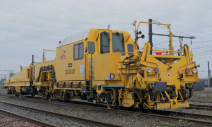
\includegraphics[width=0.96541in,height=0.57925in]{13-MAS-MS/Cours/pandoc/media/image143.png}

\textbf{BOURREUSE -- NIVELEUSE -- DRESSEUSE}


\includegraphics[width=1.35556in,height=0.38889in]{13-MAS-MS/Cours/pandoc/media/image77.png} \emph{(\ul{Source :} ATS 2020)}

\textbf{Mise en situation}

La motorisation de la bourreuse doit permettre son fonctionnement en mode circulation et en mode travail. Ces deux modes de fonctionnement sont cependant radicalement différents :

\begin{quote}
--- en mode circulation, le moteur travaille principalement en régime stabilisé et sous forte puissance ;

--- en mode travail, la puissance demandée au moteur est plus faible et le régime de fonctionnement du moteur change sans cesse.
\end{quote}

Pour qu'elle puisse tracter un convoi de 100 tonnes à la vitesse de 100 km/h (cas d'utilisation le plus énergivore), la bourreuse est pourvue d'un moteur à combustion interne dont la puissance nominale est de 486 kW. En mode travail, la puissance requise pour le fonctionnement de l'engin est significativement plus faible. Il en résulte qu'en mode travail, la motorisation de la bourreuse n'est pas exploitée de manière optimale.

\textsc{Solution envisagée.} Afin de réduire la consommation énergétique de la bourreuse en mode travail, il est envisagé d'en électrifier le fonctionnement. Chacun des trois essieux de la bourreuse sera donc pourvu d'une machine électrique. Cette évolution permettra également de réduire les émissions sonores et le niveau de vibration de la bourreuse en mode travail, améliorant ainsi le confort et la sécurité des personnels opérant sur ou à proximité de l'engin.

\textbf{Dimensionnement des modulateurs}

Afin de minimiser les modifications de la bourreuse introduites par l'électrification de sa traction, les machines électriques sont installées à la place des moteurs hydrauliques utilisés actuellement pour la traction en mode travail (figure 1). Les réducteurs situés en aval de ces moteurs sont également remplacés afin d'adapter la chaîne d'énergie à sa nouvelle motorisation.

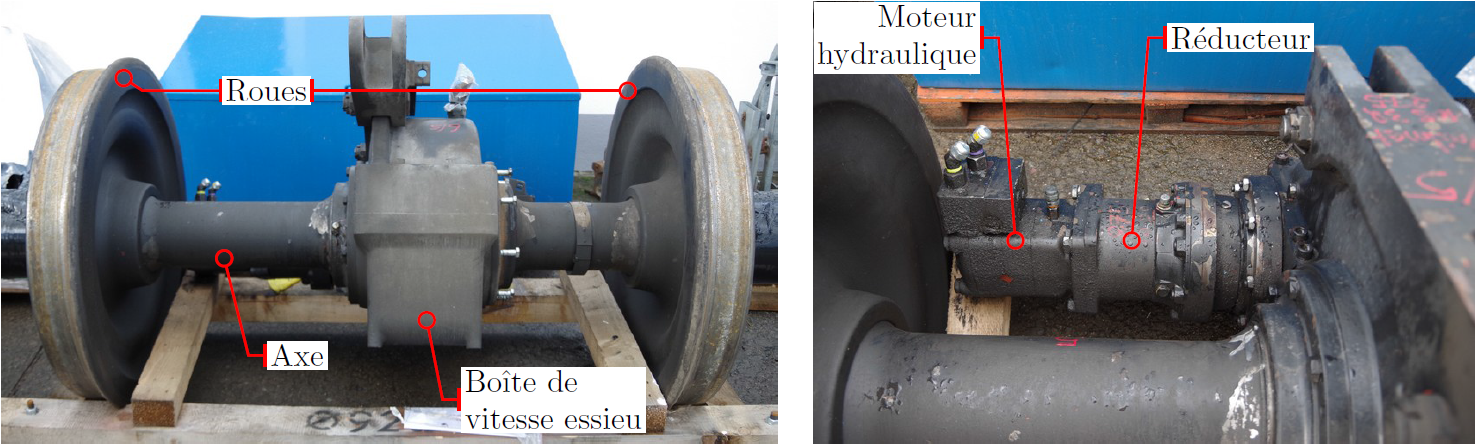
\includegraphics[width=7.33459in,height=2.20755in]{13-MAS-MS/Cours/pandoc/media/image144.png}

Figure 1 -- Vue d'un essieu, de sa boîte de vitesse et de la motorisation hydraulique

\textsc{Caractéristiques des machines}. Les machines utilisées pour la traction de la bourreuse en mode travail sont des machines synchrones triphasées à aimants permanents. Chacune de ces trois machines est alimentée par un onduleur de courant. Les données constructeur relatives à ces machines sont données dans le tableau page suivante.

\begin{longtable}[]{@{}
  >{\raggedright\arraybackslash}p{(\columnwidth - 4\tabcolsep) * \real{0.6351}}
  >{\raggedright\arraybackslash}p{(\columnwidth - 4\tabcolsep) * \real{0.1486}}
  >{\raggedright\arraybackslash}p{(\columnwidth - 4\tabcolsep) * \real{0.1892}}@{}}
\toprule\noalign{}
\begin{minipage}[b]{\linewidth}\raggedright
Grandeur
\end{minipage} & \begin{minipage}[b]{\linewidth}\raggedright
Symbole
\end{minipage} & \begin{minipage}[b]{\linewidth}\raggedright
Valeur
\end{minipage} \\
\midrule\noalign{}
\endhead
\bottomrule\noalign{}
\endlastfoot
Nombre de phases & & 3 \\
Couplage & & étoile \\
Nombres de paires de pôles & p & 4 \\
Fréquence électrique nominale & f\textsubscript{n} & 120 Hz \\
Puissance nominale & P\textsubscript{n} & 23 kW \\
Vitesse nominale & N\textsubscript{n} & 1800 tr/min \\
Tension de couplage nominale & U\textsubscript{n} & 400 V \\
Intensité nominale & I\textsubscript{n} & 42,90 A \\
Couple nominal & C\textsubscript{n} & 122 N·m \\
Rendement au point de fonctionnement nominal & η\textsubscript{n} & 0,94 \\
Intensité maximale & I\textsubscript{Max} & 62,21 A \\
Couple maximal & C\textsubscript{Max} & 164,7 N·m \\
\end{longtable}

\textbf{\ul{Modélisation et détermination des paramètres des machines}}

Les trois machines étant identiques et sollicitées de la même manière, l'étude se focalise sur une seule machine.

\textsc{Modèle électrique}. On utilise le modèle de Behn-Eschenburg pour estimer les grandeurs électriques nécessaires au fonctionnement de la machine. Ce modèle et les notations associées sont rappelés figure 2. Le système de tension triphasé est supposé équilibré et une seule phase de la machine est considérée. La résistance d'induit R et l'inductance L sont supposés constants quel que soit le point de fonctionnement de la machine.

\textsc{Dissipations de puissance}. Les seules dissipations de puissance considérées dans la machine sont les pertes cuivre modélisées par la résistance d'induit R. Les pertes magnétiques et mécaniques sont négligées.

\begin{longtable}[]{@{}
  >{\raggedright\arraybackslash}p{(\columnwidth - 2\tabcolsep) * \real{0.2195}}
  >{\raggedright\arraybackslash}p{(\columnwidth - 2\tabcolsep) * \real{0.7561}}@{}}
\toprule\noalign{}
\begin{minipage}[b]{\linewidth}\raggedright
\end{minipage} & \begin{minipage}[b]{\linewidth}\raggedright
Définition
\end{minipage} \\
\midrule\noalign{}
\endhead
\bottomrule\noalign{}
\endlastfoot
ω & Pulsation électrique en rad/s \\
\ul{V} & Tension d'alimentation d'une phase \\
\ul{I} & Courant absorbé par phase \\
R & Résistance d'induit \\
X & Réactance cyclique (X = L·ω) \\
\ul{E} & force électromotrice (fem) induite \\
\end{longtable}

Figure 2 -- Modèle électrique d'une phase d'une machine, paramètres et diagramme vectoriel associés

\textbf{1.} À partir des données constructeur, \textbf{exprimer} et \textbf{calculer} pour le point de fonctionnement nominal~:

\begin{quote}
--- la valeur efficace V\textsubscript{n} de la tension d'alimentation \ul{V} d'une phase de la machine,

--- la puissance mécanique P\textsubscript{m} délivrée par la machine,

--- la puissance électrique active P\textsubscript{abs} qu'elle absorbe.
\end{quote}

\textbf{2. Déduire} de la question précédente~:

\begin{quote}
--- le facteur de puissance de la machine à son point de fonctionnement nominal : cos(ϕ\textsubscript{n}),

--- la résistance R d'une phase d'induit.
\end{quote}

\textbf{3. Calculer} la valeur de la puissance réactive Q\textsubscript{abs} absorbée par la machine à son point de fonctionnement nominal.

\textsc{Hypothèse sur l'angle} Ψ. On suppose pour les deux questions suivantes que la fem \ul{E} est en phase avec le courant \ul{I}, c'est à dire que Ψ = 0.

\textbf{4. Exprimer} la puissance réactive Q\textsubscript{abs} absorbée par la machine en fonction notamment de la réactance cyclique X. \textbf{En déduire} la valeur de l'inductance cyclique L.

\textsc{Constante de couplage}. La valeur efficace de la fem E est proportionnelle à la vitesse de rotation Ω\textsubscript{m} de la machine~: E~=~K·Ω\textsubscript{m}.

\textbf{5. Déterminer} l'expression de la constante de couplage K et donner sa valeur dans les unités du système international.

\textbf{\ul{Grandeurs électriques maximales en entrée de la machine}}

\textsc{Couple délivré par la machine}. On admet que le couple C\textsubscript{m} délivré par une machine synchrone à aimants peut, dans le cadre des hypothèses de l'étude, s'exprimer par la relation suivante (les notations de la figure 2 sont conservées) :

C\textsubscript{m} = 3·K·cos(Ψ)·I

\textsc{Points de fonctionnement visés}. La détermination des grandeurs électriques maximales en entrée de la machine passe par l'étude de deux points de fonctionnement particuliers : le décollage et la fin de la phase d'accélération.

\begin{quote}
--- Au décollage de la bourreuse (mise en marche à partir de la vitesse nulle), les phénomènes d'adhérence imposent d'appliquer un effort de traction plus important que lorsque la bourreuse est en mouvement. Ce point de fonctionnement impose le courant maximal absorbé par la machine. Lors du décollage de la bourreuse, la machine délivre un couple C\textsubscript{mdec} = 140 N·m.

--- À la fin de la phase d'accélération, la machine délivre un couple C\textsubscript{mfa} = 115 N·m et tourne à la vitesse N\textsubscript{fa}~=~1700~tr/min.
\end{quote}

\textsc{Paramètres électriques de la machine}. Il est rappelé que le modèle électrique de la machine est donné figure 2. Quels que soient les résultats trouvés précédemment, on utilisera les valeurs suivantes dans la suite de cette étude~:

R = 0,27 Ω ; L = 4,1 mH ; K = 0,95 V·s/rad

\textsc{Pilotage de la machine}. L'onduleur qui alimente la machine est asservi pour maintenir l'angle Ψ (angle d'autopilotage) à 0.

\textbf{6. Expliquer} l'intérêt de maintenir l'angle Ψ à 0.

\textbf{7.} En supposant Ψ = 0, \textbf{calculer} le courant efficace I\textsubscript{dec} absorbé par la machine lors du décollage de la bourreuse.

\textbf{8.} En supposant Ψ = 0, \textbf{calculer} le courant efficace I\textsubscript{fa} absorbé par la machine et la tension efficace V\textsubscript{fa} aux bornes d'une de ses phases à la fin de la phase d'accélération.

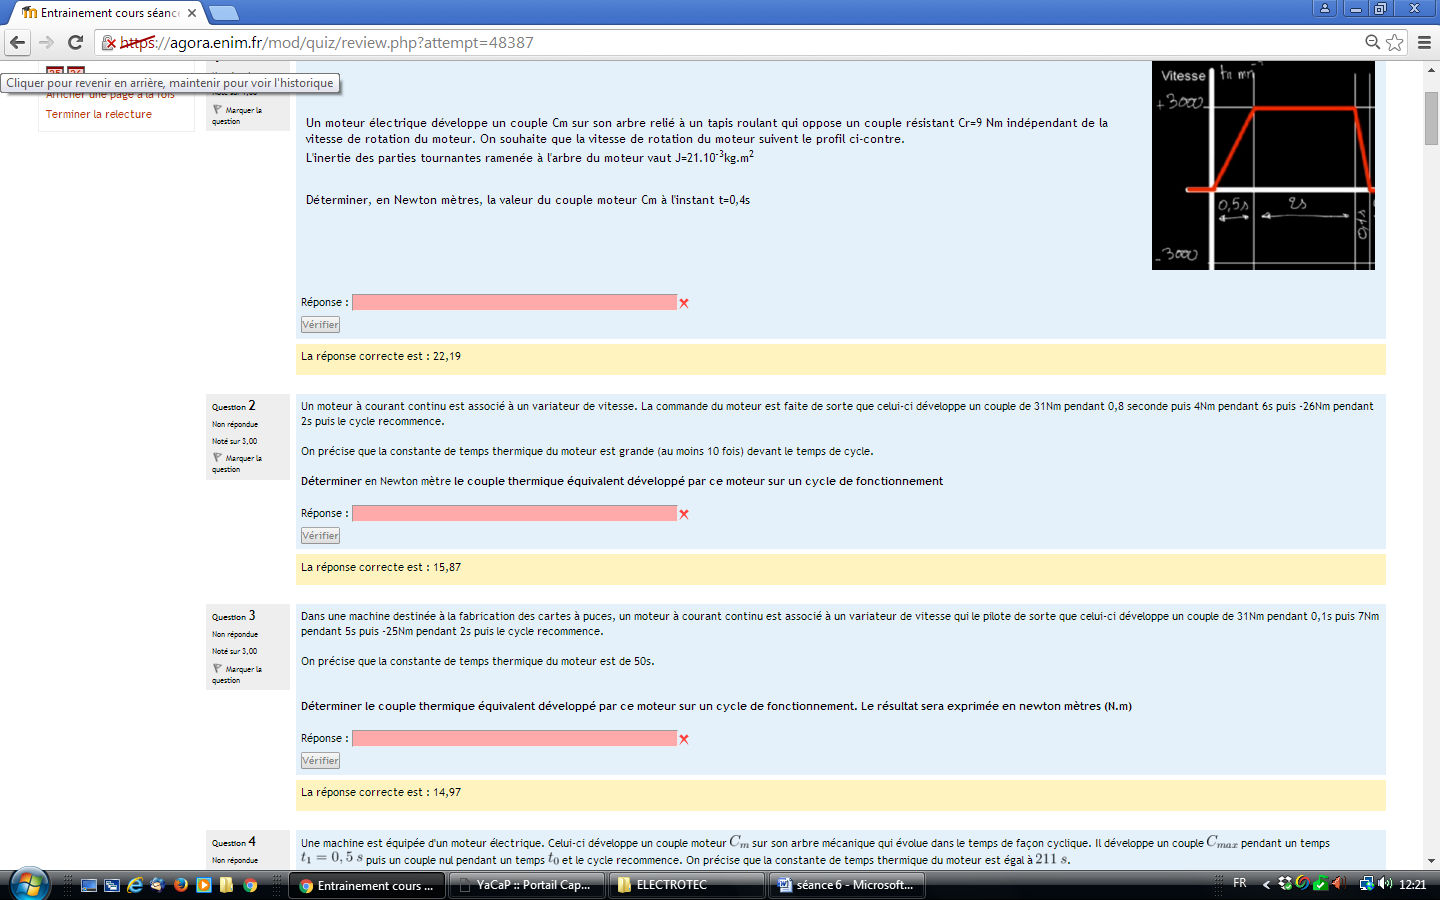
\includegraphics[width=7.24525in,height=1.50141in]{13-MAS-MS/Cours/pandoc/media/image145.png}

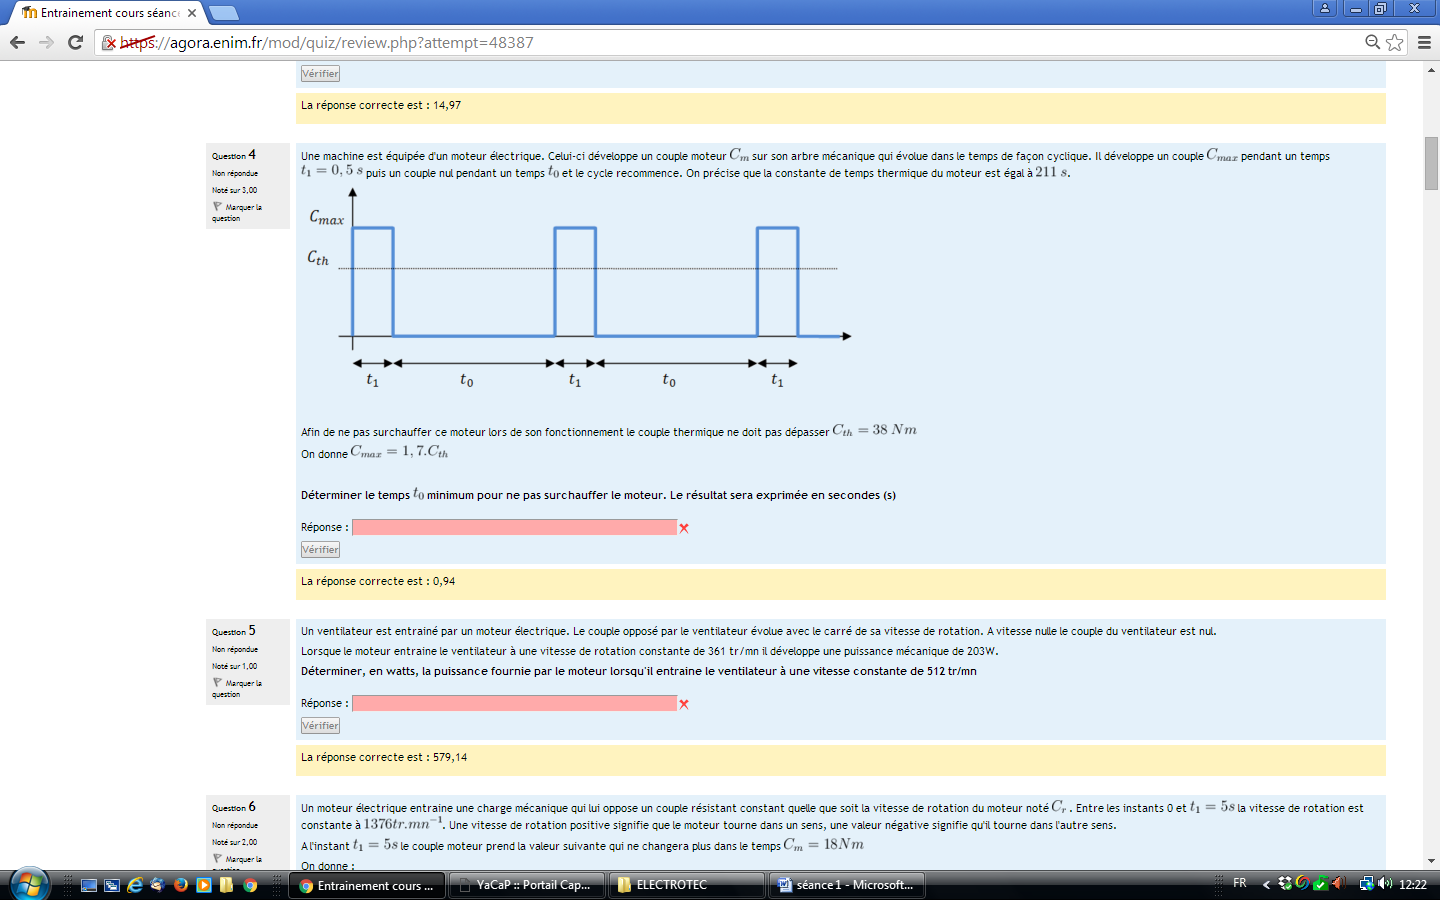
\includegraphics[width=7.11899in,height=3.03858in]{13-MAS-MS/Cours/pandoc/media/image146.png}

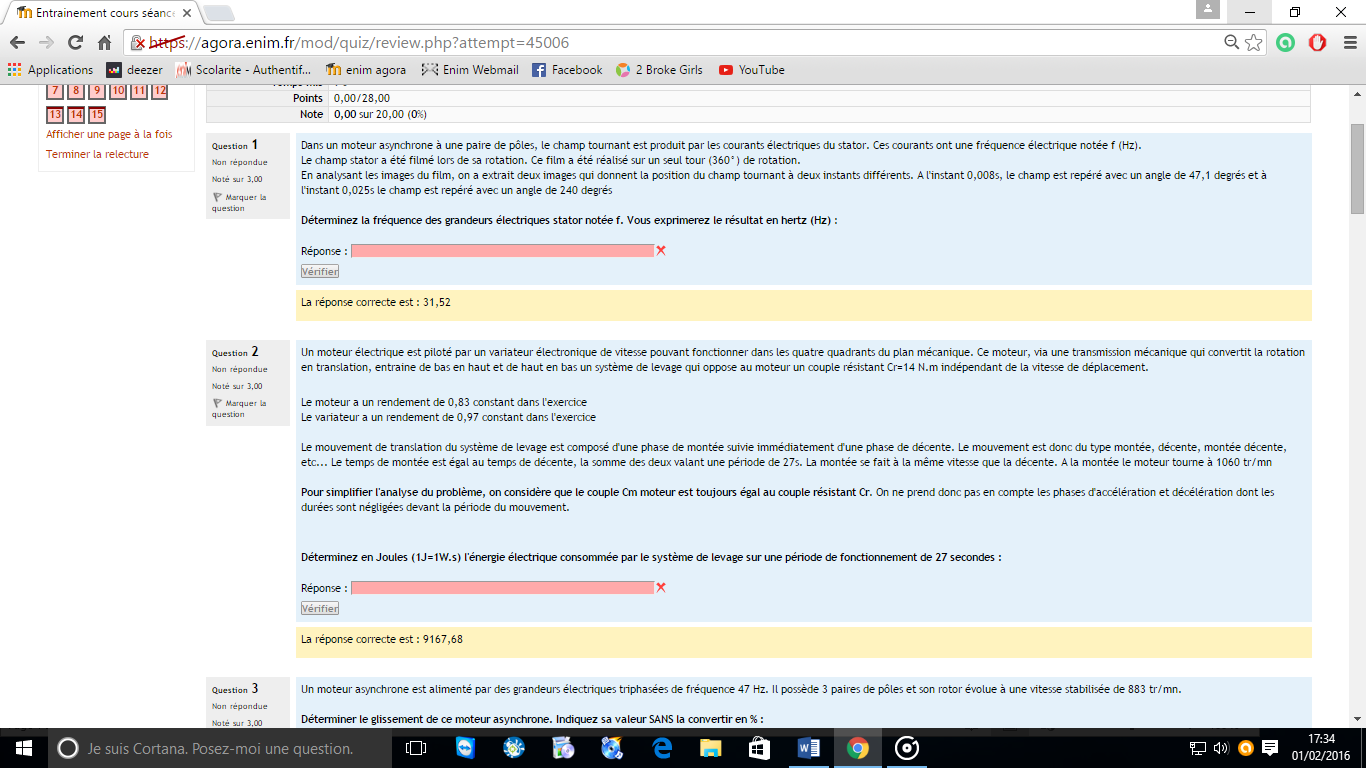
\includegraphics[width=7.21829in,height=3.72601in]{13-MAS-MS/Cours/pandoc/media/image147.png}

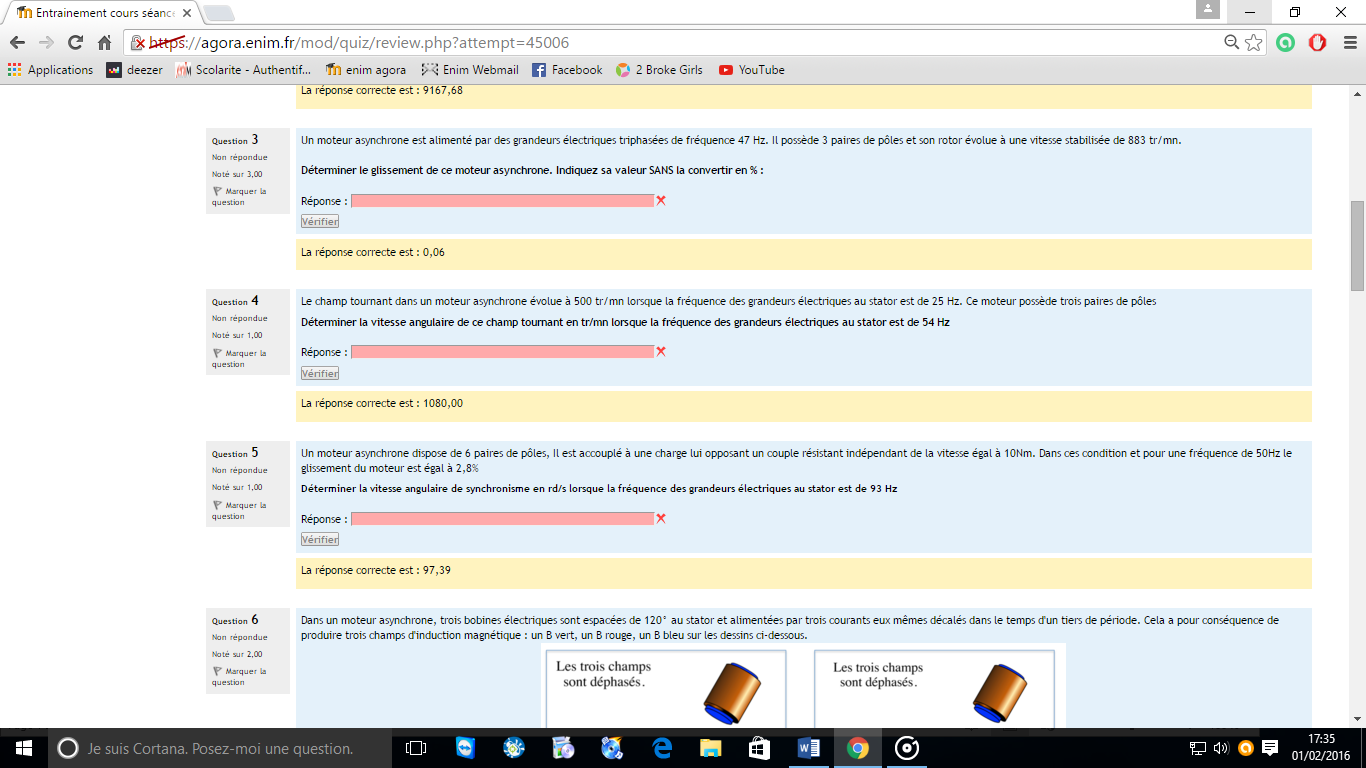
\includegraphics[width=7.16591in,height=3.23222in]{13-MAS-MS/Cours/pandoc/media/image148.png}

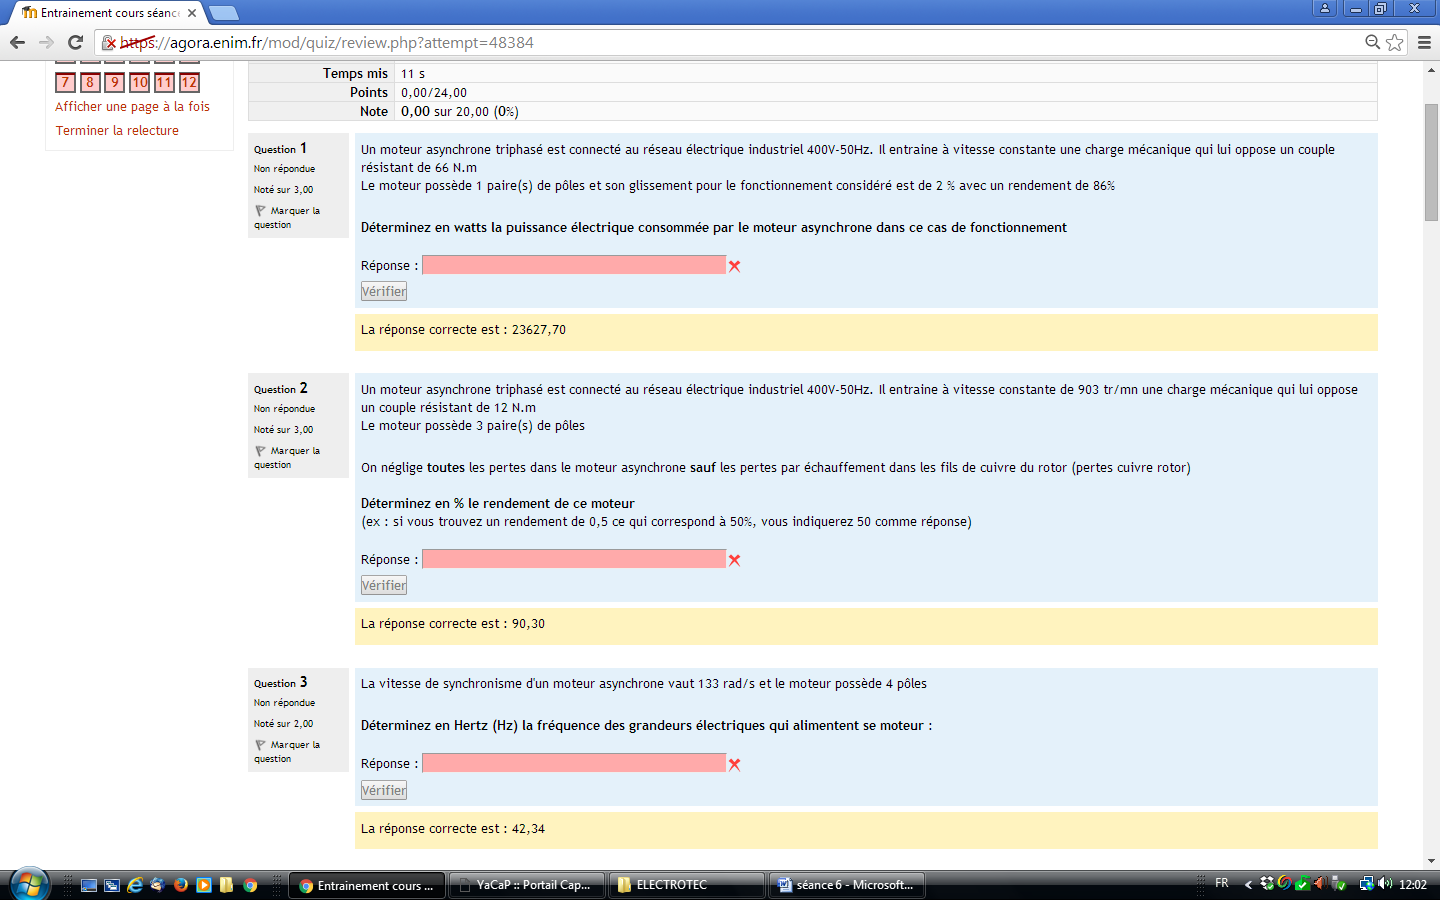
\includegraphics[width=7.23493in,height=4.97837in]{13-MAS-MS/Cours/pandoc/media/image149.png}

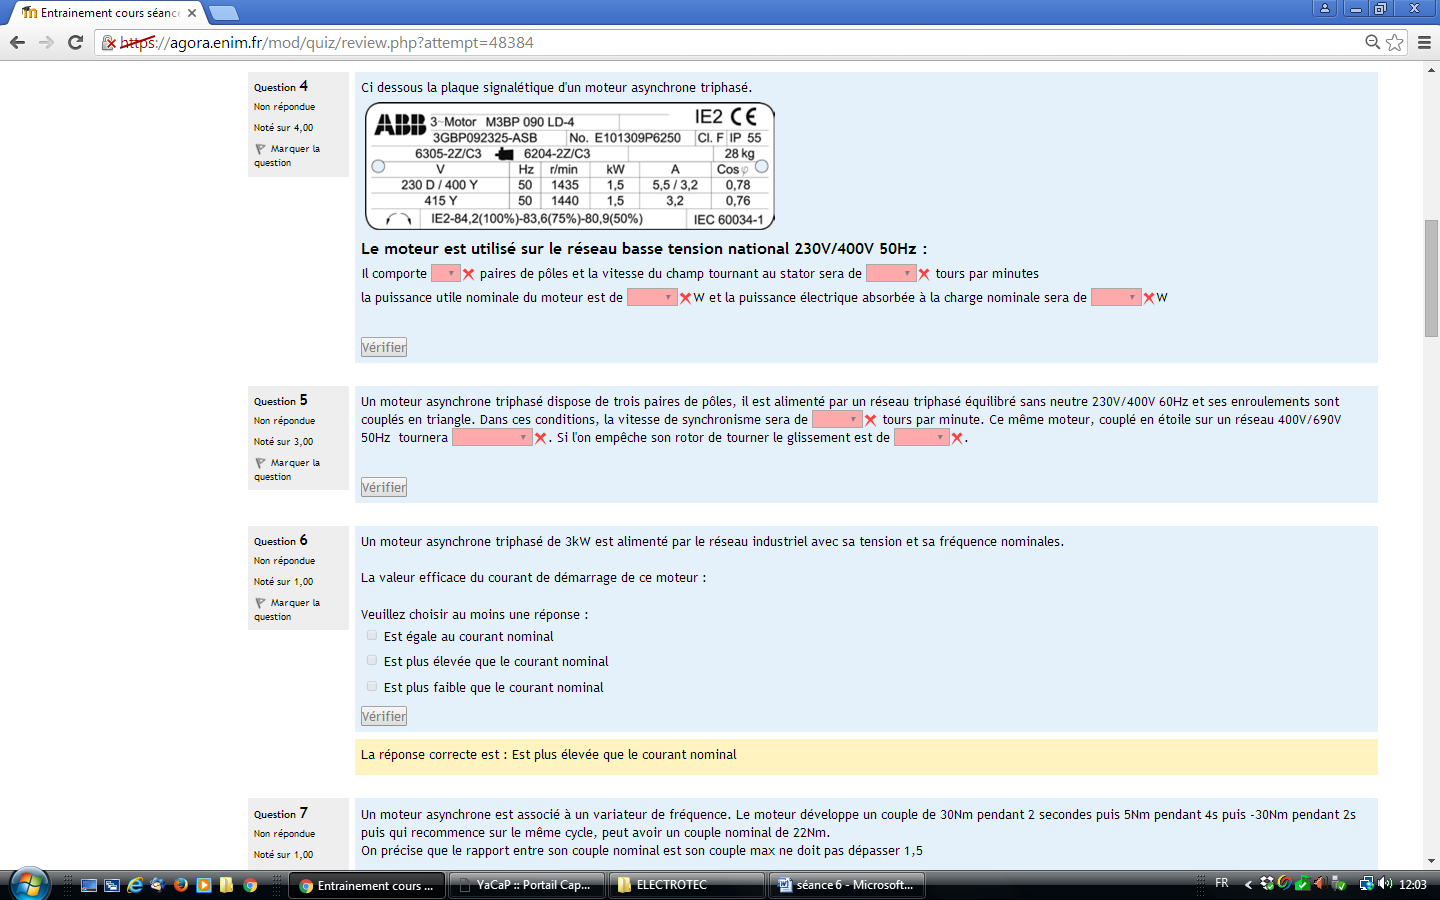
\includegraphics[width=7.195in,height=4.93584in]{13-MAS-MS/Cours/pandoc/media/image150.png}

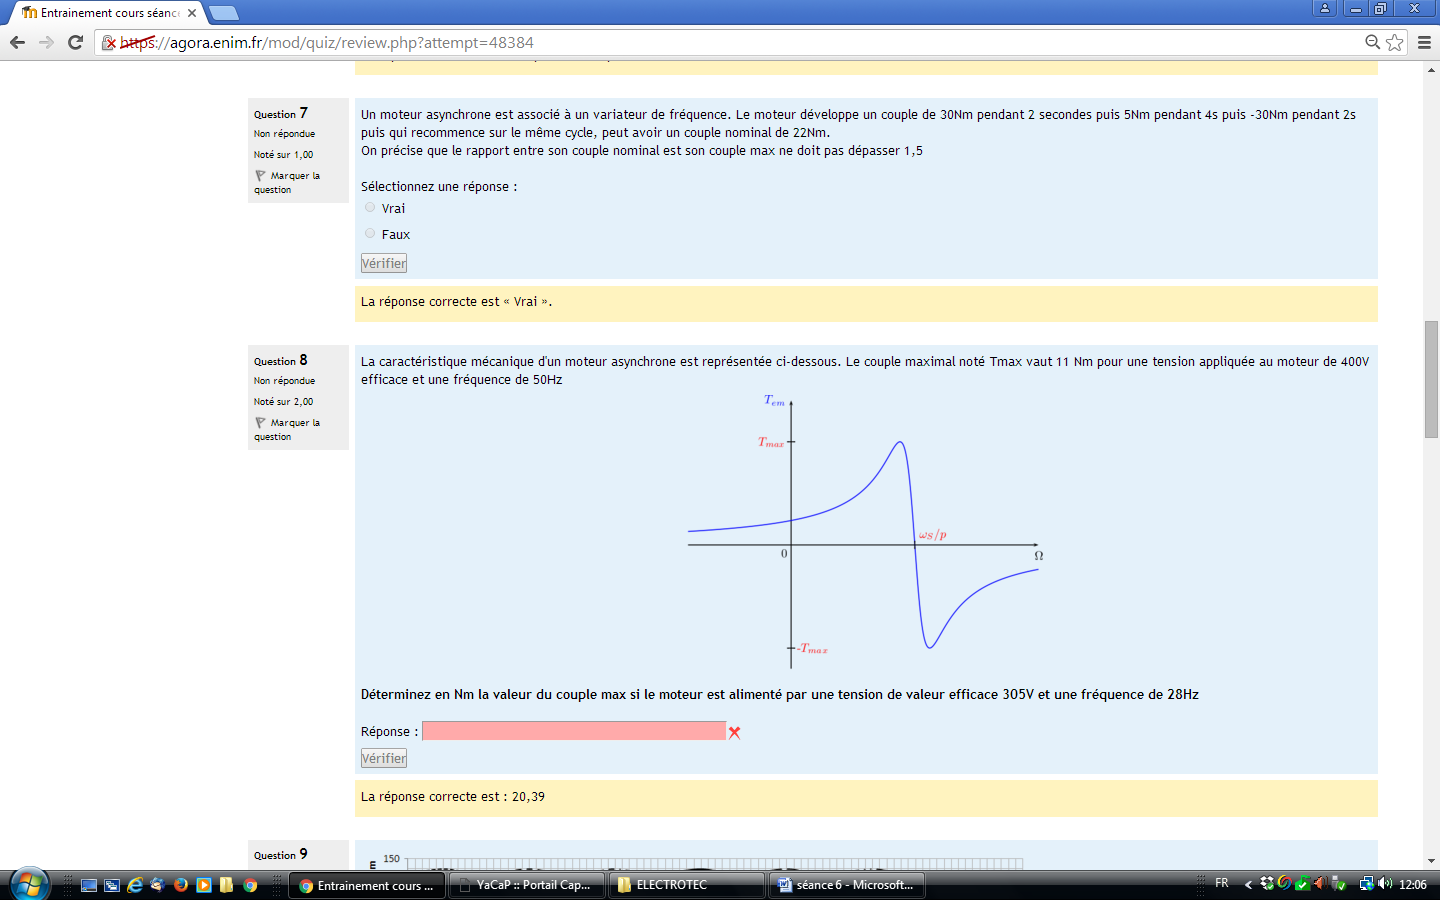
\includegraphics[width=7.35165in,height=5.10845in]{13-MAS-MS/Cours/pandoc/media/image151.png}

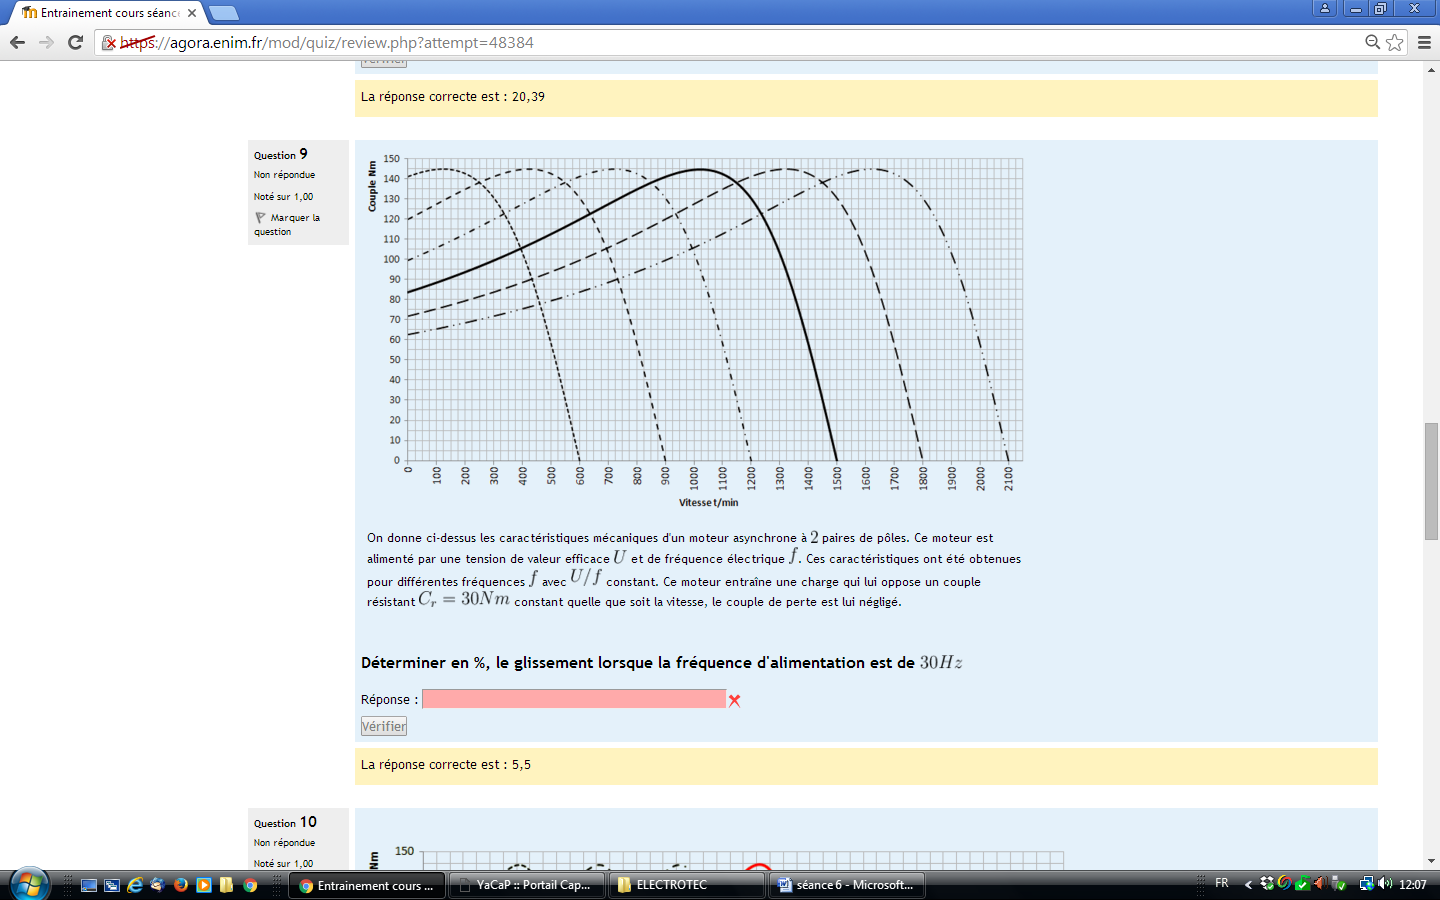
\includegraphics[width=7.3074in,height=4.86808in]{13-MAS-MS/Cours/pandoc/media/image152.png}

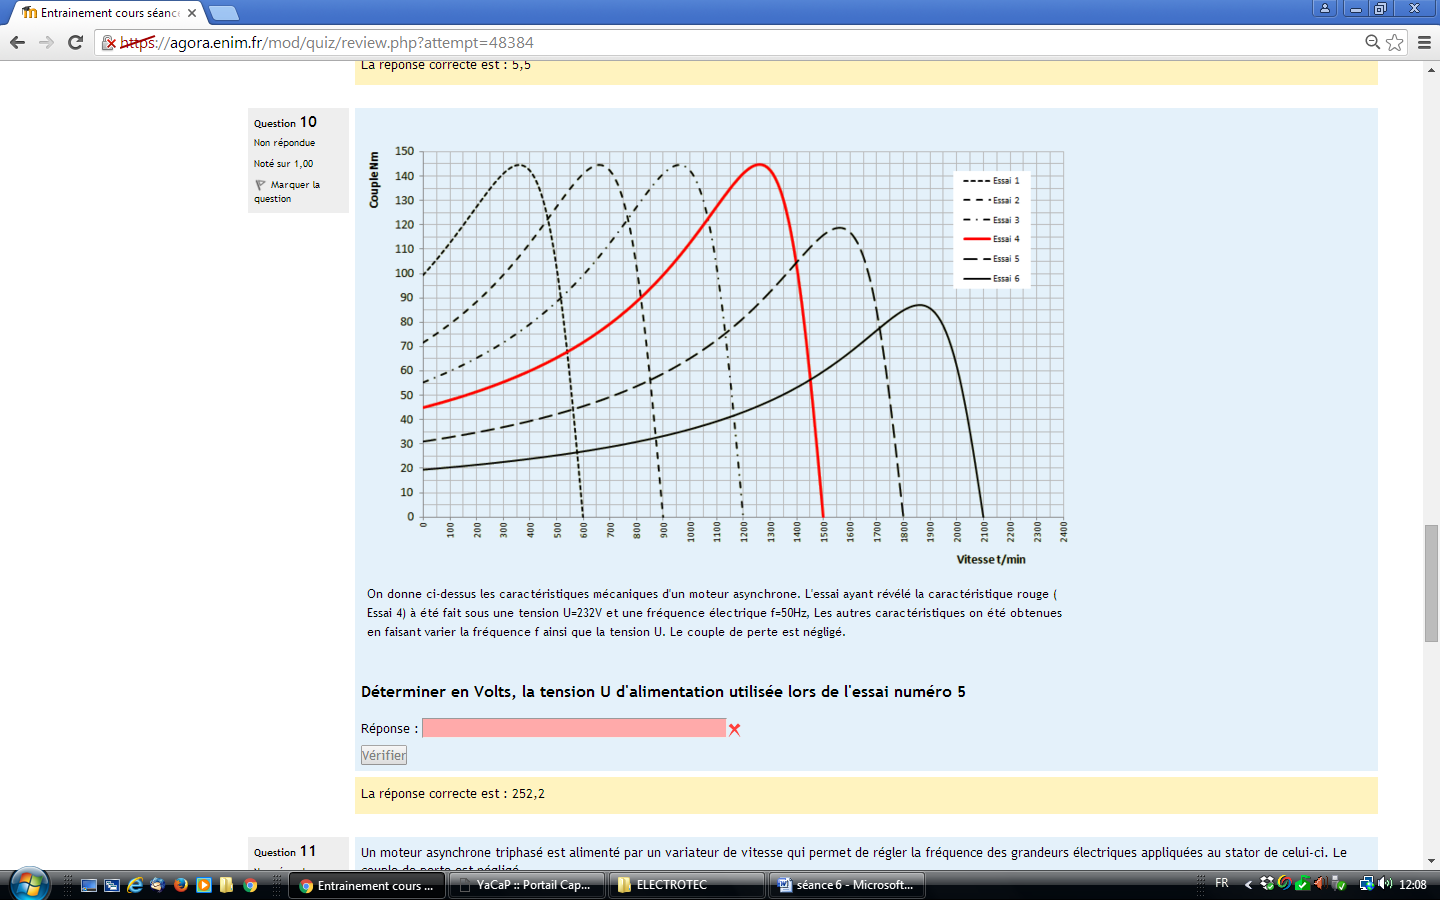
\includegraphics[width=7.08366in,height=4.96154in]{13-MAS-MS/Cours/pandoc/media/image153.png}

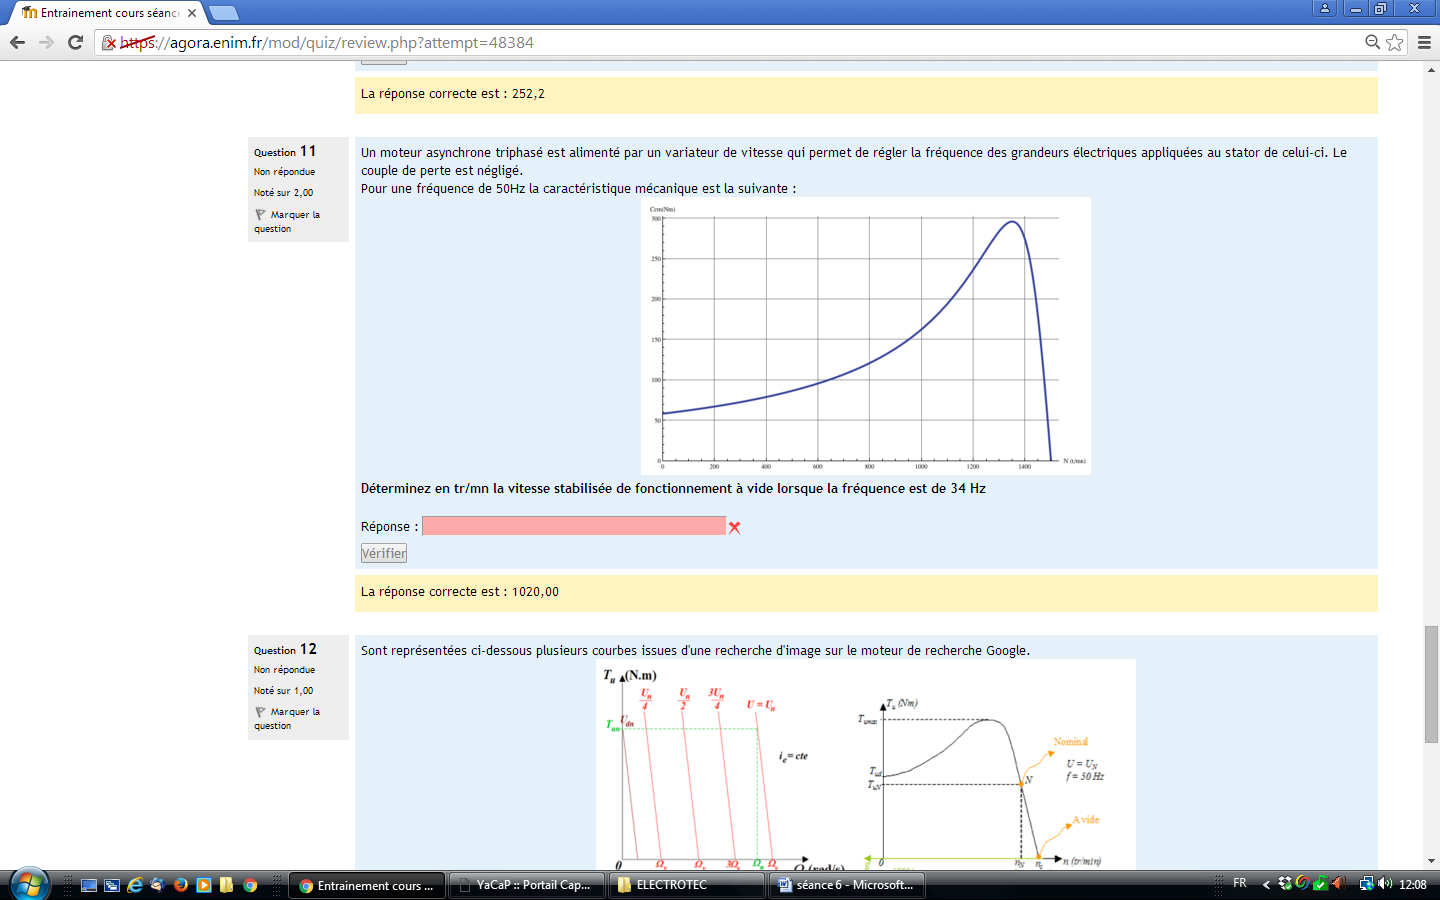
\includegraphics[width=7.11183in,height=3.2676in]{13-MAS-MS/Cours/pandoc/media/image154.png}

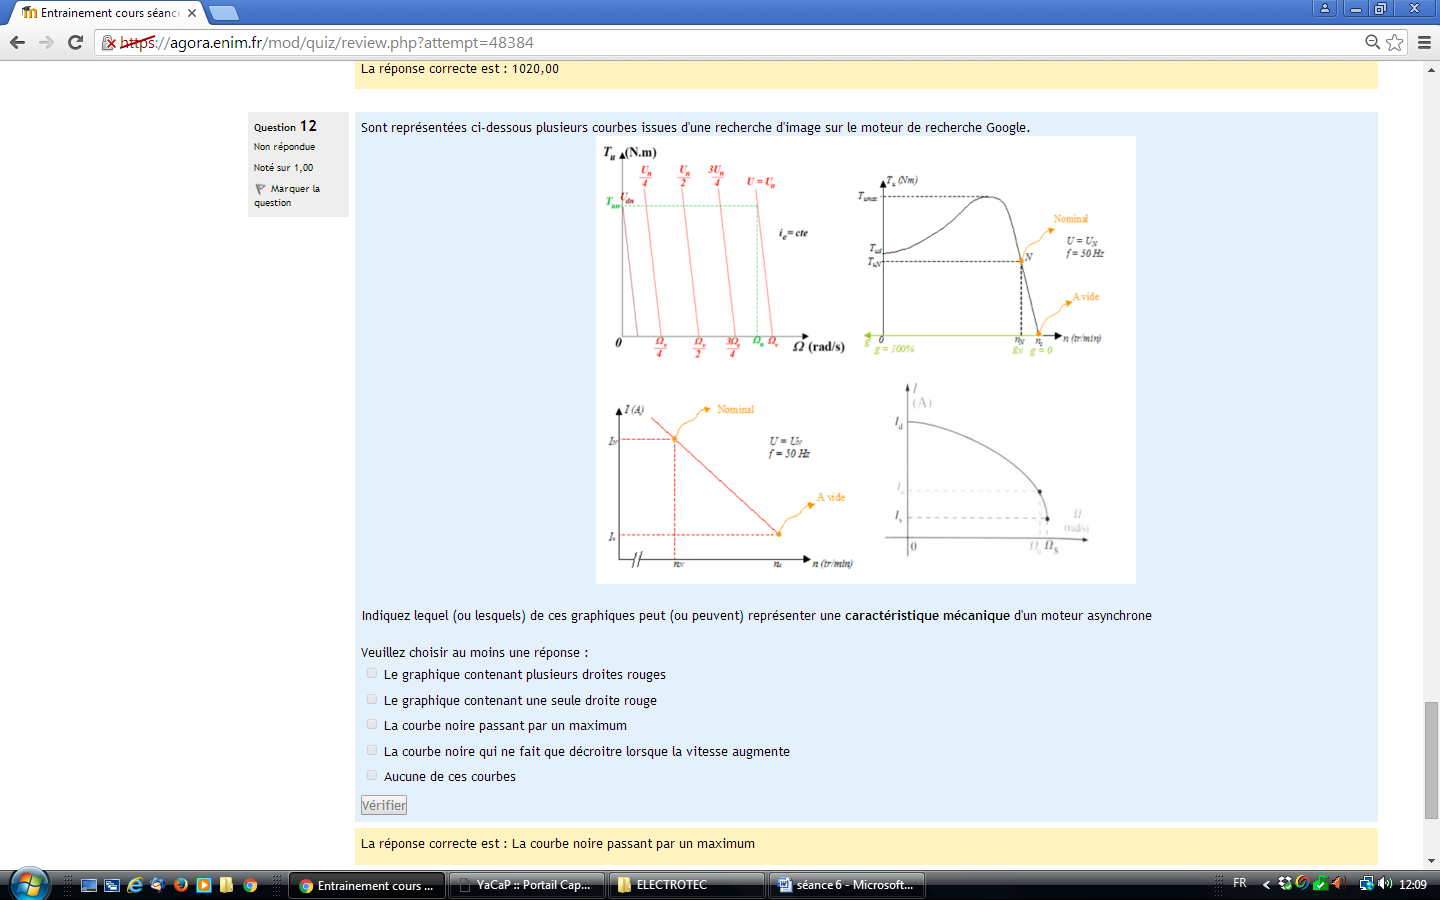
\includegraphics[width=7.32715in,height=5.17863in]{13-MAS-MS/Cours/pandoc/media/image155.png}


\includegraphics[width=6.82708in,height=4.55139in]{13-MAS-MS/Cours/pandoc/media/image156.emf}


\includegraphics[width=7.26806in,height=4.22917in]{13-MAS-MS/Cours/pandoc/media/image157.emf}


\includegraphics[width=7.26806in,height=3.23333in]{13-MAS-MS/Cours/pandoc/media/image158.emf}


\includegraphics[width=7.26806in,height=4.32778in]{13-MAS-MS/Cours/pandoc/media/image159.emf}


\includegraphics[width=7.26806in,height=3.86528in]{13-MAS-MS/Cours/pandoc/media/image160.emf}


\includegraphics[width=7.26806in,height=4.67222in]{13-MAS-MS/Cours/pandoc/media/image161.emf}
\includegraphics[width=7.26806in,height=1.31736in]{13-MAS-MS/Cours/pandoc/media/image162.emf}

\begin{center}\rule{0.5\linewidth}{0.5pt}\end{center}

\hypertarget{inventaire-des-images}{%
\subsection{Inventaire des images}\label{inventaire-des-images}}

13-MAS-MS/Cours/pandoc/media/image1.png 13-MAS-MS/Cours/pandoc/media/image10.jpeg 13-MAS-MS/Cours/pandoc/media/image100.png 13-MAS-MS/Cours/pandoc/media/image101.wmf 13-MAS-MS/Cours/pandoc/media/image102.wmf 13-MAS-MS/Cours/pandoc/media/image103.wmf 13-MAS-MS/Cours/pandoc/media/image104.png 13-MAS-MS/Cours/pandoc/media/image105.png 13-MAS-MS/Cours/pandoc/media/image106.png 13-MAS-MS/Cours/pandoc/media/image107.emf 13-MAS-MS/Cours/pandoc/media/image108.emf 13-MAS-MS/Cours/pandoc/media/image109.png 13-MAS-MS/Cours/pandoc/media/image11.png 13-MAS-MS/Cours/pandoc/media/image110.png 13-MAS-MS/Cours/pandoc/media/image111.png 13-MAS-MS/Cours/pandoc/media/image112.emf 13-MAS-MS/Cours/pandoc/media/image113.emf 13-MAS-MS/Cours/pandoc/media/image114.png 13-MAS-MS/Cours/pandoc/media/image115.png 13-MAS-MS/Cours/pandoc/media/image116.png 13-MAS-MS/Cours/pandoc/media/image117.jpeg 13-MAS-MS/Cours/pandoc/media/image118.png 13-MAS-MS/Cours/pandoc/media/image119.png 13-MAS-MS/Cours/pandoc/media/image12.png 13-MAS-MS/Cours/pandoc/media/image120.wmf 13-MAS-MS/Cours/pandoc/media/image121.wmf 13-MAS-MS/Cours/pandoc/media/image123.png 13-MAS-MS/Cours/pandoc/media/image124.png 13-MAS-MS/Cours/pandoc/media/image125.png 13-MAS-MS/Cours/pandoc/media/image126.png 13-MAS-MS/Cours/pandoc/media/image127.png 13-MAS-MS/Cours/pandoc/media/image128.emf 13-MAS-MS/Cours/pandoc/media/image13.png 13-MAS-MS/Cours/pandoc/media/image130.png 13-MAS-MS/Cours/pandoc/media/image131.png 13-MAS-MS/Cours/pandoc/media/image132.emf 13-MAS-MS/Cours/pandoc/media/image133.emf 13-MAS-MS/Cours/pandoc/media/image134.emf 13-MAS-MS/Cours/pandoc/media/image135.emf 13-MAS-MS/Cours/pandoc/media/image136.jpeg 13-MAS-MS/Cours/pandoc/media/image137.png 13-MAS-MS/Cours/pandoc/media/image138.png 13-MAS-MS/Cours/pandoc/media/image139.png 13-MAS-MS/Cours/pandoc/media/image14.png 13-MAS-MS/Cours/pandoc/media/image140.emf 13-MAS-MS/Cours/pandoc/media/image141.emf 13-MAS-MS/Cours/pandoc/media/image142.emf 13-MAS-MS/Cours/pandoc/media/image143.png 13-MAS-MS/Cours/pandoc/media/image144.png 13-MAS-MS/Cours/pandoc/media/image145.png 13-MAS-MS/Cours/pandoc/media/image146.png 13-MAS-MS/Cours/pandoc/media/image147.png 13-MAS-MS/Cours/pandoc/media/image148.png 13-MAS-MS/Cours/pandoc/media/image149.png 13-MAS-MS/Cours/pandoc/media/image15.png 13-MAS-MS/Cours/pandoc/media/image150.png 13-MAS-MS/Cours/pandoc/media/image151.png 13-MAS-MS/Cours/pandoc/media/image152.png 13-MAS-MS/Cours/pandoc/media/image153.png 13-MAS-MS/Cours/pandoc/media/image154.png 13-MAS-MS/Cours/pandoc/media/image155.png 13-MAS-MS/Cours/pandoc/media/image156.emf 13-MAS-MS/Cours/pandoc/media/image157.emf 13-MAS-MS/Cours/pandoc/media/image158.emf 13-MAS-MS/Cours/pandoc/media/image159.emf 13-MAS-MS/Cours/pandoc/media/image16.emf 13-MAS-MS/Cours/pandoc/media/image160.emf 13-MAS-MS/Cours/pandoc/media/image161.emf 13-MAS-MS/Cours/pandoc/media/image162.emf 13-MAS-MS/Cours/pandoc/media/image17.png 13-MAS-MS/Cours/pandoc/media/image18.png 13-MAS-MS/Cours/pandoc/media/image19.png 13-MAS-MS/Cours/pandoc/media/image20.gif 13-MAS-MS/Cours/pandoc/media/image21.png 13-MAS-MS/Cours/pandoc/media/image22.png 13-MAS-MS/Cours/pandoc/media/image23.png 13-MAS-MS/Cours/pandoc/media/image24.emf 13-MAS-MS/Cours/pandoc/media/image26.emf 13-MAS-MS/Cours/pandoc/media/image27.emf 13-MAS-MS/Cours/pandoc/media/image28.jpeg 13-MAS-MS/Cours/pandoc/media/image29.emf 13-MAS-MS/Cours/pandoc/media/image3.emf 13-MAS-MS/Cours/pandoc/media/image30.png 13-MAS-MS/Cours/pandoc/media/image32.png 13-MAS-MS/Cours/pandoc/media/image33.png 13-MAS-MS/Cours/pandoc/media/image34.wmf 13-MAS-MS/Cours/pandoc/media/image35.wmf 13-MAS-MS/Cours/pandoc/media/image36.wmf 13-MAS-MS/Cours/pandoc/media/image37.emf 13-MAS-MS/Cours/pandoc/media/image38.png 13-MAS-MS/Cours/pandoc/media/image39.png 13-MAS-MS/Cours/pandoc/media/image40.emf 13-MAS-MS/Cours/pandoc/media/image41.png 13-MAS-MS/Cours/pandoc/media/image42.jpeg 13-MAS-MS/Cours/pandoc/media/image43.wmf 13-MAS-MS/Cours/pandoc/media/image44.wmf 13-MAS-MS/Cours/pandoc/media/image45.wmf 13-MAS-MS/Cours/pandoc/media/image46.wmf 13-MAS-MS/Cours/pandoc/media/image47.wmf 13-MAS-MS/Cours/pandoc/media/image48.png 13-MAS-MS/Cours/pandoc/media/image49.wmf 13-MAS-MS/Cours/pandoc/media/image5.png 13-MAS-MS/Cours/pandoc/media/image50.wmf 13-MAS-MS/Cours/pandoc/media/image51.wmf 13-MAS-MS/Cours/pandoc/media/image52.png 13-MAS-MS/Cours/pandoc/media/image53.png 13-MAS-MS/Cours/pandoc/media/image54.png 13-MAS-MS/Cours/pandoc/media/image55.png 13-MAS-MS/Cours/pandoc/media/image56.png 13-MAS-MS/Cours/pandoc/media/image57.png 13-MAS-MS/Cours/pandoc/media/image58.png 13-MAS-MS/Cours/pandoc/media/image59.png 13-MAS-MS/Cours/pandoc/media/image6.png 13-MAS-MS/Cours/pandoc/media/image60.jpeg 13-MAS-MS/Cours/pandoc/media/image61.wmf 13-MAS-MS/Cours/pandoc/media/image62.emf 13-MAS-MS/Cours/pandoc/media/image63.emf 13-MAS-MS/Cours/pandoc/media/image64.emf 13-MAS-MS/Cours/pandoc/media/image65.wmf 13-MAS-MS/Cours/pandoc/media/image66.wmf 13-MAS-MS/Cours/pandoc/media/image67.wmf 13-MAS-MS/Cours/pandoc/media/image68.wmf 13-MAS-MS/Cours/pandoc/media/image69.wmf 13-MAS-MS/Cours/pandoc/media/image7.png 13-MAS-MS/Cours/pandoc/media/image70.wmf 13-MAS-MS/Cours/pandoc/media/image71.wmf 13-MAS-MS/Cours/pandoc/media/image72.wmf 13-MAS-MS/Cours/pandoc/media/image73.wmf 13-MAS-MS/Cours/pandoc/media/image74.emf 13-MAS-MS/Cours/pandoc/media/image75.wmf 13-MAS-MS/Cours/pandoc/media/image76.png 13-MAS-MS/Cours/pandoc/media/image77.png 13-MAS-MS/Cours/pandoc/media/image78.png 13-MAS-MS/Cours/pandoc/media/image79.png 13-MAS-MS/Cours/pandoc/media/image8.wmf 13-MAS-MS/Cours/pandoc/media/image80.png 13-MAS-MS/Cours/pandoc/media/image81.png 13-MAS-MS/Cours/pandoc/media/image82.png 13-MAS-MS/Cours/pandoc/media/image83.png 13-MAS-MS/Cours/pandoc/media/image84.png 13-MAS-MS/Cours/pandoc/media/image85.png 13-MAS-MS/Cours/pandoc/media/image86.jpeg 13-MAS-MS/Cours/pandoc/media/image87.png 13-MAS-MS/Cours/pandoc/media/image88.jpeg 13-MAS-MS/Cours/pandoc/media/image9.png 13-MAS-MS/Cours/pandoc/media/image90.wmf 13-MAS-MS/Cours/pandoc/media/image91.jpeg 13-MAS-MS/Cours/pandoc/media/image92.png 13-MAS-MS/Cours/pandoc/media/image93.jpeg 13-MAS-MS/Cours/pandoc/media/image94.jpeg 13-MAS-MS/Cours/pandoc/media/image95.png 13-MAS-MS/Cours/pandoc/media/image96.png 13-MAS-MS/Cours/pandoc/media/image97.jpeg 13-MAS-MS/Cours/pandoc/media/image98.png 13-MAS-MS/Cours/pandoc/media/image99.png
